\def\coursename{电动力学}
\def\courseEnglishname{Electrodynamics}
\def\teachername{唐传祥、邢庆子}
\def\beginday{2023/2/22}
\def\endday{2023/6/16}

\documentclass[a4paper, 11pt]{article}

\usepackage[UTF8]{ctex}

\usepackage[T1]{fontenc}								% 字体
\catcode`\。=\active
\newcommand{。}{.} % {\ifmmode\text{.}\else .\fi}
\catcode`\(=\active
\catcode`\)=\active
\newcommand{(}{(}
\newcommand{)}{)}

% \usepackage{zhlineskip}

\usepackage{nicematrix}
% \usepackage{setspace}
% \linespread{1}						% 一倍行距
\setlength{\headheight}{14pt}			% 页眉高度
% \setlength{\lineskip}{0ex}			% 行距
\renewcommand\arraystretch{.82}		% 表格

\usepackage{amssymb, amsmath, amsfonts, amsthm}			% 数学符号,公式,字体,定理环境
\everymath{\displaystyle}			% \textstyle \scriptstyle \scriptscriptstyle
\allowdisplaybreaks[4]      		% 使用行间公式格式
% \makeatletter
% \renewcommand{\maketag@@@}[1]{\hbox{\m@th\normalsize\normalfont#1}}
% \makeatother
\newif\ifcontent\contenttrue		% if 显示目录
\newif\ifparskip\parskipfalse		% if 增加目录后的行距
\newif\ifshowemail\showemailfalse	% if 显示 email
\def\firstandforemost{
	\maketitle
	%\thispagestyle{empty}\clearpage
	\ifcontent
		\renewcommand{\contentsname}{目录}
		\tableofcontents
		\thispagestyle{empty}
		\clearpage
	\fi
	\ifparskip
		\setlength{\parskip}{.8ex}	% 设置额外的段距,目录后
	\fi								% 在 \firstandforemost 前设置 \parskiptrue
	\makenomenclature
	\printnomenclature
	\setcounter{page}{1}
}

\usepackage{mathtools}									% \rcase 环境等

% \usepackage{physics}

\usepackage[]{siunitx}									% 国际制单位
\sisetup{
	inter-unit-product = \ensuremath{{}\cdot{}},
	per-mode = symbol,
	per-mode = reciprocal-positive-first,
	range-units = single,
	separate-uncertainty = true,
	range-phrase = \ifmmode\text{\;-\;}\else\;-\;\fi
}
\DeclareSIUnit\angstrom{\text{Å}}
\DeclareSIUnit\atm{\text{atm}}
% SIunits 额外定义了一个 \square 表示平方,
% 还会把 \cdot 空格加大,真有够无语的 😅

\usepackage{authblk}									% 作者介绍
\ifx \coursefullname\undefined
	\ifx \coursename\undefined
		\def\coursename{笔记}
	\fi
	\def\coursefullname{\coursename}
\fi
\ifx \authorname\undefined
	\def\authorname{Dait}
\fi
\ifx \departmentname\undefined
	\def\departmentname{THU}
\fi
\ifx \emailaddress\undefined
	\def\emailaddress{daiyj20@mails.tsinghua.edu.cn}
\fi
\ifx \beginday\undefined
	\def\beginday{2021}
\fi
\ifx \endday\undefined
	\def\endday{\number\year/\number\month/\number\day}
\fi
\ifx \titleannotation\undefined
	\ifx \teachername\undefined
		\title{\textbf{\coursefullname}}
	\else
		\title{\textbf{\coursefullname}\\\small\textit{主要整理自\teachername 老师讲义}}
	\fi
\else
	\title{\textbf{\coursefullname}\\\small\textit{(\titleannotation)}}
\fi
\newif\ifdefaultauthor\defaultauthortrue
\ifdefaultauthor
	\author{by~\authorname~at~\departmentname}
	\ifshowemail
		\affil{\emailaddress}
	\fi
\fi
\ifx \endday\beginday
	\date{\beginday}
\else
	\date{\beginday~-~\endday}
\fi

\usepackage{hyperref}									% 链接
\ifx \courseEnglishname\undefined
	\def\courseEnglishname{Note}
\fi
\ifx \authorEnglishname\undefined
	\def\authorEnglishname{Dait}
\fi
\hypersetup{
	% dvipdfm								% 表示用 dvipdfm 生成 pdf
	pdftitle={\coursename},
	pdfauthor={\authorname},
	colorlinks=true, breaklinks=true,		% 超链接设置
	linkcolor=black, citecolor=black, urlcolor=blue
}

\usepackage[british]{babel}								% 长单词自动连字符换行
\hyphenation{long-sen-ten-ce}				% 自定义拆分方式

\usepackage{tikz}
\usetikzlibrary{quotes, angles}
\usepackage{pgfplots}
\pgfplotsset{compat=1.17}								% TikZ
\newcommand{\coor}[5][0]{
	\draw[thick,latex-latex](#1,#3)node[left]{$#5$}--(#1,0)node[shift={(-135:7pt)}]{$O$}--(#1+#2,0)node[right]{$#4$}
}			% 坐标轴

\usepackage{enumerate}									% 编号
\usepackage{paralist}
\setlength{\pltopsep}{1ex}
\setlength{\plitemsep}{1ex}
\ifx \eqnrange\undefined
	\numberwithin{equation}{section}
\else
	\numberwithin{equation}{\eqnrange}
\fi

\renewcommand{\thempfootnote}{\Roman{mpfootnote}}
\renewcommand{\thefootnote}{\Roman{footnote}}		% 注释上标 I, II,...
\newcommand{\sectionstar}[1]{
	\section[\hspace{-.8em}*\hspace{.3em}#1]{\hspace{-1em}*\hspace{.5em}#1}
}
\newcommand{\subsectionstar}[1]{					% 带星号的 section 和 subsection
	\subsection{\hspace{-1em}*\hspace{.5em}#1}
}
\newcommand{\subsubsectionstar}[1]{					% 带星号的 section 和 subsection
	\subsubsection{\hspace{-1em}*\hspace{.5em}#1}
}
\newcommand*{\appendiks}{
	\appendix
	\part*{附录}
	\addcontentsline{toc}{part}{附录}
}
\iffalse			% 不清楚
	\newcommand{\varsection}[1]{
		\refstepcounter{section}
		\section*{\thesection\quad #1}
		\addcontentsline{toc}{section}{\makebox[0pt][r]{*}\thesection\quad #1}
	}
\fi

\usepackage{fancyhdr}									% 页眉页脚
\ifx \coursename\undefined
	\def\coursename{笔记}
\fi
\fancyhf{}\pagestyle{fancy}
\fancyhead[L]{\coursename\rightmark}
\fancyhead[R]{by~\authorname}
\fancyfoot[C]{-~\thepage~-} 			%页码

\usepackage{colortbl, booktabs}							% 表

\usepackage{graphicx}
\usepackage{float}
\usepackage{caption}									% 图
\captionsetup{
	margin=20pt, format=hang,
	justification=justified
}
\newcounter{tikzpic}
\def\tikzchap{
	\stepcounter{tikzpic}\\
	\small 图~\thetikzpic\quad
}
\newcounter{linetable}
\newcommand{\tablechap}[1]{
	\stepcounter{linetable}
	{\small 表~\thelinetable\quad #1}\\[1em]
}

\usepackage{tcolorbox}									% 盒子
\tcbuselibrary{theorems, skins, breakable}
\definecolor{MatchaGreen}{HTML}{73C088}		% 抹茶绿B7C6B3
\newtcbtheorem[number within = subsection]{example}{例}{
	enhanced, breakable, sharp corners,
	attach boxed title to top left = {yshifttext = -1mm},
	before skip = 2ex,
	colback = MatchaGreen!5,				% 文本框内的底色
	colframe = MatchaGreen,					% 文本框框沿的颜色
	fonttitle = \bfseries,					% 标题字体用粗体	coltitle 默认 white,
	boxed title style = {
			sharp corners, size = small, colback = MatchaGreen,
		}
}{exm}
\definecolor{MelancholyBlue}{HTML}{9EAABA}	% melancholy: 沮丧
\newcounter{pslt}
\setcounter{pslt}{-1}
\newtcbtheorem[use counter = pslt]{posulate}{假设}{
	enhanced, breakable, sharp corners,
	attach boxed title to top left = {yshifttext = -1mm}, before skip = 2ex,
	colback = MelancholyBlue!5, colframe = MelancholyBlue, fonttitle = \bfseries,
	boxed title style = {
			sharp corners, size = small, colback = MelancholyBlue,
		}
}{psl}
\definecolor{PureBlue}{HTML}{80A3D0}
\newtcbtheorem[number within = subsection]{definition}{定义}{
	enhanced, breakable, sharp corners,
	attach boxed title to top left = {yshifttext = -1mm}, before skip = 2ex,
	colback = PureBlue!5, colframe = PureBlue, fonttitle = \bfseries,
	boxed title style = {
			sharp corners, size = small, colback = PureBlue,
		}
}{dfn}
\definecolor{PeachRed}{HTML}{EA868F}
\newtcbtheorem[number within = subsection]{theorem}{定理}{
	enhanced, breakable, sharp corners,
	attach boxed title to top left = {yshifttext = -1mm}, before skip = 2ex,
	colback = PeachRed!5, colframe = PeachRed, fonttitle = \bfseries,
	boxed title style = {
			sharp corners, size = small, colback = PeachRed,
		}
}{thm}
\definecolor{SchembriumYellow}{HTML}{fbd26a}	% 申博太阳城黄
\newtcbtheorem[number within = section]{method}{方法}{
	enhanced, breakable, sharp corners,
	attach boxed title to top left = {yshifttext = -1mm}, before skip = 2ex,
	colback = SchembriumYellow!5, colframe = SchembriumYellow, fonttitle = \bfseries,
	boxed title style = {
			sharp corners, size = small, colback = SchembriumYellow,
		}
}{mtd}
% 保留颜色
\definecolor{fadedgold}{HTML}{D9CBB0}		% 褪色金
\definecolor{saturatedgold}{HTML}{F0E0C2}	% staurated: 饱和
\definecolor{elegantblue}{HTML}{C4CCD7}		% elegant: 优雅
\definecolor{ivory}{HTML}{F1ECE6}			% 象牙
\definecolor{gloomypruple}{HTML}{CCC1D2}	% 阴沉紫
% \textcolor[HTML]{FFC23A}					% 石板灰

\definecolor{Green}{rgb}{0,.8,0}

\usepackage{imakeidx}								% 索引

\usepackage{nomencl}								% 关键词
%\setlength{\nomitemsep}{0.2cm}							% 设置术语之间的间距
\renewcommand{\nomentryend}{.}							% 设置打印出术语的结尾的字符
\renewcommand{\eqdeclaration}[1]{见公式:(#1)}			% 设置打印见公式的样式
\renewcommand{\pagedeclaration}[1]{见第 (#1) 页}		% 设置打印页的样式
\renewcommand{\nomname}{术语表} 						% 修改术语表标题的名称。

\usepackage{array}
\usepackage{booktabs} % 三线表
\usepackage{multirow}
% 手动排版,尽量杜绝使用

\newcommand{\bs}[1]{\hspace{-#1 pt}}		% 手动减间距	backspace
\newcommand{\bv}[1]{\vspace{-#1 pt}}		% 手动缩行距	backvspace
\def\directlisteqn{\vspace{-1ex}}
\iffalse									% 尽量避免孤行
	\widowpenalty=4000
	\clubpenalty=4000
\fi

% 杂项符号
\def\avg{\overline}
\newcommand*{\rqed}{\tag*{$\square$}}								% 靠右 QED
\newcommand*{\halfqed}{\tag*{$\boxdot$}}
\newcommand*{\thus}{\quad\Rightarrow\quad}							% =>
\newcommand*{\ifnf}{\quad\Leftrightarrow\quad}						% <=>	if and only if
\newcommand*{\turnto}{\quad\to\quad}
\newcommand*{\normalize}{\quad\overset{\mathrm{normalize}}{-\!\!\!-\!\!\!-\!-\!\!\!\longrightarrow}\quad}
\newcommand*{\vthus}{\\$\Downarrow$\\}
\newcommand*{\viff}{\\$\Updownarrow$\\}
\newcommand*{\vs}{~\text{-}~}
\newcommand{\eg}[1][]{\subparagraph*{例#1:}}
\newcommand*{\prf}{\noindent\textbf{证明:}\quad}
\newcommand{\dpfr}[2]{\displaystyle\frac{#1}{#2}}					% 大分数
\newcommand{\frdp}[2]{\frac{\displaystyle #1}{\displaystyle #2}}
\newcommand{\spark}[1]{\;\textcolor{red}{#1}}

% 简化更常用的希腊字母
\newcommand*{\vf}{\varphi}
\newcommand*{\vF}{\varPhi}
\newcommand*{\vp}{\varPsi}
\newcommand*{\ve}{\varepsilon}
\newcommand*{\vC}{\varTheta}
\newcommand*{\ct}{\theta}			% 还是建议用 @ + Tab 快捷键

% 正体符号
\newcommand*{\cns}{\mathrm{const}}
\newcommand*{\plusc}{{\color{lightgray}\,+\,\cns}}
\newcommand*{\e}{\mathop{}\!\mathrm{e}^}	% e
\let\accenti\i
\renewcommand*{\i}{\mathrm{i}}
\newcommand*{\D}{\Delta}
\newcommand*{\p}{\partial}

\usepackage{bm}											% 粗体 \bm
\newcommand{\hbm}[1][r]{\hat{\bm #1}}	% 应该不会有两个字母的
\newcommand{\ibm}[1]{\,\bm #1}

% Using EnglischeSchT script font style
\newfontfamily{\calti}{EnglischeSchT}
\newcommand{\mathcalti}[1]{\mbox{\calti{#1}}}
\newcommand{\mathcaltibf}[1]{\mbox{\bf\calti{#1}}}

\usepackage{mathrsfs}									% 花体 \mathscr
% \usepackage{boondox-cal}								% 小写花体 \mathcal
\newcommand*{\RR}{\mathbb R}
\newcommand*{\CC}{\mathbb C}
\newcommand*{\ZZ}{\mathbb Z}
\newcommand*{\sC}{\mathscr C}			% n 阶连续可导函数
\newcommand*{\sR}{\mathscr R}			% 黎曼可积
% 算符用 \mathcal
\newcommand*{\cL}{\mathcal L}			% 表示一般算子
\newcommand{\cl}[1]{\mathcal L\fkh{#1}}
\newcommand{\cli}[1]{\mathcal L^{-1}\!\fkh{#1}}
\newcommand{\cf}[2][\!\,]{\mathcal F_\mathrm{#1}\fkh{#2}}
\newcommand{\cfi}[2][\!\,]{\mathcal F_\mathrm{#1}^{-1}\!\fkh{#2}}
% \newcommand{\cl}[2][0]{\mathcal L\ikh[#1]{#2}}
% \newcommand{\cli}[2][0]{\mathcal L^{-1}\ikh[#1]{#2}}
% \newcommand{\cf}[2][0]{\mathcal F\ikh[#1]{#2}}
% \newcommand{\cfi}[2][0]{\mathcal F^{-1}\ikh[#1]{#2}}

\usepackage{cancel}										% 删除线

\usepackage{xfrac}

% \usepackage{emoji}	需要 LuaTeX

% 导数等
\let\divides\div
\renewcommand*{\div}{\nabla\cdot}
\newcommand*{\curl}{\nabla\times}
\newcommand*{\lap}{\Delta}
\let\accentd\d
\renewcommand*{\d}{\mathop{}\!\mathrm{d}}
\newcommand*{\nd}{\mathrm{d}}
\newcommand*{\vd}{\mathop{}\!\delta}											% δ
\newcommand{\dd}[2][\;\!\!]{\frac{\nd^{#1}}{\nd #2^{#1}}}						% d/dx			我知道 \,\! 很愚蠢,但是 {} 无法在 Math Preview 上预览
\newcommand{\dn}[2]{\frac{\nd^{#1}}{\nd #2^{#1}}}								% d^n/dx^n		\dn2x≡\dd[2]x
\newcommand{\dv}[3][\;\!\!]{\frac{\nd^{#1}#2}{\nd #3^{#1}}}						% df/dx
\newcommand{\du}[3]{\frac{\nd^{#1}#2}{\nd #3^{#1}}}								% d^nf/dx^n		\du2fx≡\dv[2]fx
\newcommand{\pp}[2][\;\!\!]{\frac{\p^{#1}}{\p #2^{#1}}}							% ∂/∂x
\newcommand{\pn}[2]{\frac{\p^{#1}}{\p #2^{#1}}}									% ∂^n/∂x^n		\pn2x≡\pp[2]x
\newcommand{\pv}[3][\;\!\!]{\frac{\p^{#1}#2}{\p #3^{#1}}}						% ∂f/∂x
\newcommand{\pu}[3]{\frac{\p^{#1}#2}{\p #3^{#1}}}								% ∂^nf/∂x^n		\pu2x≡\pv[2]x
\newcommand{\pw}[3]{\frac{\p^2 #1}{\p #2\p #3}}									% ∂^2f/∂x∂y
\newcommand{\pvv}[6]{															% ∂^(m+n)f/∂x^m∂y^n
	\ifnum#4=1
		\ifnum#6=1
			\frac{\p^{#1}#2}{\p #3\p #5}
		\else
			\frac{\p^{#1}#2}{\p #3\p #5^{#6}}
		\fi
	\else
		\ifnum#6=1
			\frac{\p^{#1}#2}{\p #3^{#4}\p #5}
		\else
			\frac{\p^{#1}#2}{\p #3^{#4}\p #5^{#6}}
		\fi
	\fi}
\newcommand{\dvd}[2]{\left.#1\middle\slash #2\right.}							% 斜除

% 积分
\newcommand*{\intt}{\bs2\int\bs8\int}											% ∫∫
\newcommand*{\inttt}{\int\bs8\int\bs8\int}										% ∫∫∫
\newcommand*{\intdt}{\int\bs3\cdot\bs2\cdot\bs2\cdot\bs4\int}					% ∫...∫
\newcommand*{\zti}{_0^{+\infty}}												% _0^+∞
\newcommand*{\iti}{_{-\infty}^{+\infty}}										% _-∞^+∞
\newcommand{\fmto}[3][\infty]{_{#2=#3}^{#1}}

% 括号
\newcommand{\abs}[1]{\left\lvert#1\right\rvert}									% |x| 绝对值
\newcommand{\norm}[1]{\left\lVert#1\right\rVert}								% ||x|| 模
\newcommand{\edg}[1]{\left.#1\right\rvert}										% f|  竖线
\newcommand{\kh}[1]{\left(#1\right)}											% (x) 括号
\newcommand{\fkh}[1]{\left[#1\right]}											% [x] 方括号
\newcommand{\hkh}[1]{\left\{#1\right\}}											% {x} 花括号
\newcommand{\zkh}[1]{\lfloor\bs{4.7}\lceil #1\rceil\bs{4.7}\rfloor}				% [x] 中括号
\newcommand{\ikh}[2][0]{\ifnum#1=0 \zkh{#2}\else \fkh{#2}\fi}					% [x] 可调大小的中括号
\newcommand{\set}[2]{\left\{#1\,\middle\vert\,#2\right\}}						% {x|x1,x2,...} 集合
\newcommand{\ave}[1]{\left\langle #1\right\rangle}								% <x> 平均值
\newcommand{\bra}[1]{\left\langle #1\right\vert}								% <ψ| 左矢
\newcommand{\ket}[1]{\left\vert #1\right\rangle}								% |ψ> 右矢
\newcommand{\brkt}[2]{\left\langle #1\middle\vert #2\right\rangle}				% <φ|ψ> 内积
\newcommand{\ktbr}[2]{\left\vert#1\right\rangle \bs3\left\langle #2\right\vert}	% |ψ><φ|
\newcommand{\inp}[2]{\left\langle #1,#2\right\rangle}							% <f,g> 内积

% 数学运算符
\let\Real\Re
\let\Imagin\Im
\let\Re\relax
\let\Im\relax
\DeclareMathOperator{\Re}{Re}					% 
\DeclareMathOperator{\Im}{Im}					% 
\DeclareMathOperator{\sech}{sech}				% 
\DeclareMathOperator{\csch}{csch}				% 
\DeclareMathOperator{\arcsec}{arcsec}			% 
\DeclareMathOperator{\arccot}{arccot}			% 
\DeclareMathOperator{\arccsc}{arccsc}			% 
\DeclareMathOperator{\arsinh}{arsinh}			% 
\DeclareMathOperator{\arcosh}{arcosh}			% 
\DeclareMathOperator{\artanh}{artanh}			% 
\DeclareMathOperator{\sgn}{sgn}					% 符号函数
\DeclareMathOperator{\Li}{Li}					% 
\DeclareMathOperator{\Si}{Si}
\DeclareMathOperator{\Ci}{Ci}
\DeclareMathOperator{\sinc}{sinc}
\DeclareMathOperator{\Heaviside}{H}
\DeclareMathOperator{\arr}{A}					% 排列数
\DeclareMathOperator{\com}{C}					% 组合数
\DeclareMathOperator{\Res}{Res}					% 留数
\DeclareMathOperator{\supp}{supp}
\newcommand*{\bigo}{\mathcal O}

% 线性代数
\newif\ifLinearAlgebra\LinearAlgebratrue
\ifLinearAlgebra
\DeclareMathOperator{\rank}{rank}
\DeclareMathOperator{\id}{id}
\newcommand*{\tp}{^{\mathrm T}}				% AT 转置
\newcommand*{\cj}{^\ast}					% A* 共轭
\newcommand*{\dg}{^\dagger}					% A† 共轭转置
\newcommand*{\iv}{^{-1}}					% A-1
\fi

% 物理学家
\newcommand*{\Schr}{Schrödinger}
\newcommand*{\Legd}{Legendre}
\newcommand*{\deB}{de Broglie}
\newcommand*{\Rayl}{Rayleigh}
\newcommand*{\Lande}{Landé}

% 粒子
\newcommand*{\elc}{\mathrm e}
\newcommand*{\pton}{\mathrm p}
\newcommand*{\mol}{\mathrm m}

% 物理常数
\newcommand*{\NA}{N_{\bs1\mathrm A}}						% Avogadro 常数
\newcommand*{\kB}{k_{\mathrm B}}							% Boltzmann 常数
\newcommand*{\muB}{\mu_\mathrm B}							% Bohr 磁矩

% 
\newcommand*{\Ek}{E_{\mathrm k}}							% 动能
\newcommand*{\eff}{_\mathrm{eff}}							% 有效下标
\newcommand*{\tot}{_\mathrm{tot}}
\newcommand*{\lSI}{\tag{SI}}
\newcommand*{\CGS}{\tag{CGS}}								% cm, g, s 制

\sisetup{separate-uncertainty = false}
\newcommand*{\lapla}{\nabla^2}
\renewcommand*{\r}{\text r}
\renewcommand*{\t}{\text t}
\renewcommand*{\c}{_\text c}
%\newcommand*{\vr}{\varepsilon_\r}
\newcommand*{\emf}{\mathcal{E}}

\begin{document}

\firstandforemost
本课基于John David Jackson的Classical Electrodynamics和David J. Griffiths的Introduction to Electrodynamics。
其中除第 \ref{sec:vector analysis} 章矢量分析和第 \ref{sec:relativistic electromagnetic} 章相对论电动力学是参考Griffiths书外,其余均参考Jackson书。本笔记将Jackson书中的Chap. 2, 3: Boundary-Value Problems in Electrostatics: I, II合并为了一章:第 \ref{sec:boundary-value problems} 章静电学中的边界条件问题。

在Jackson书的Introduction中,着重强调了以下关键词:
\begin{compactitem}
	\item force-field
	\item classical-quantum
	\item linear-nonlinear
	\item mathmetical idealization-truly physics
	\item space-time
	\item macroscopic-microscopic
\end{compactitem}

\clearpage
\setcounter{section}{-1}
\section{矢量分析}
\label{sec:vector analysis}
\subsection{矢量代数}
\begin{compactitem}
	\item 定义:标量和矢量。
	\item 矢量的运算:加法、数乘、标量积、矢量积(平凡的)。
	\item 标量三重积
    \begin{align}
        \bm A\cdot(\bm B\times\bm C)&=\bm C\cdot(\bm A\times\bm B)=(\bm A\times\bm B)\cdot\bm C\\\notag
        &=\begin{vmatrix}
            A_x&A_y&A_z\\
            B_x&B_y&B_z\\
            C_x&C_y&C_z
        \end{vmatrix}.
    \end{align}
    \item 矢量三重积:back cab规则
    \begin{align}
        \label{eqn:bac-cab}
        \bm A\times(\bm B\times\bm C)&=\bm B(\bm A\cdot\bm C)-\bm C(\bm A\cdot\bm B);\\
        (\bm A\times\bm B)\times\bm C&=\bm B(\bm A\cdot\bm C)-\bm A(\bm B\cdot\bm C).
    \end{align}
    可以将多个矢量积简化,比如
    \begin{align*}
        (\bm A\times\bm B)\cdot(\bm C\times\bm D)&=(\bm A\cdot\bm C)(\bm B\cdot\bm D)-(\bm A\cdot\bm D)(\bm B\cdot\bm C).
    \end{align*}
    \item 位置向量和分离向量
    \item 向量转换
\end{compactitem}
\subsection{微分}
\begin{compactitem}
	\item 常微分
    \[
        \d f=\dv fx\d x.
    \]
	\item 标量场$f(x,y,z)$的微分
    \begin{align}
        \d f=\pv fx\d x+\pv fy\d y+\pv fz\d z=:\nabla f\cdot\d\bm\ell.
    \end{align}
    梯度(gradient)
    \begin{align}
        \nabla f:=\pv fx\uvec x+\pv fy\uvec y+\pv fz\uvec z.
    \end{align}
	\item Hamiltonian
	\begin{align}
        \nabla:=\pp x\uvec x+\pp y\uvec y+\pp z\uvec z.
    \end{align}
    \item 散度(divergence)
    \begin{align}
        \div\bm A=\pv{A_x}x+\pv{A_y}y+\pv{A_z}z.
    \end{align}
    \item 旋度(curl)
    \begin{align}\notag
        &\curl\bm A=\begin{vmatrix}
            \uvec x&\uvec y&\uvec z\\
            \pp x&\pp y&\pp z\\
            A_x&A_y&A_z
        \end{vmatrix}\\
        &=\biggkh{\pv{A_z}y-\pv{A_y}z}\uvec x+\biggkh{\pv{A_x}z-\pv{A_z}x}\uvec y+\biggkh{\pv{A_y}x-\pv{A_x}y}\uvec z.
    \end{align}
\end{compactitem}
\paragraph{乘法法则}
\begin{compactitem}
	\item 常微分乘法法则
    \[
        \d(fg)=(\d f)g+f\d g.
    \]
    \item 梯度、旋度、散度的简单乘法法则
    \begin{align}
        \nabla(fg)&=(\nabla f)g+f\nabla g;\\
        \div(f\bm A)&=(\nabla f)\cdot\bm A+f(\div\bm A);\\
        \curl(f\bm A)&=(\nabla f)\times\bm A+f(\curl\bm A).
    \end{align}
    \item 梯度、旋度、散度的复杂乘法法则
    \begin{align}
        \notag
        \nabla(\bm A\cdot\bm B)&=\bm A\times(\curl\bm B)+\bm B\times(\curl\bm A)+\\
        \label{eqn:gradA.B}
        &\qquad(\bm A\cdot\nabla)\bm B+(\bm B\cdot\nabla)\bm A;\\
        \label{eqn:divAxB}
        \div(\bm A\times\bm B)&=(\curl\bm A)\cdot\bm B-(\curl\bm B)\cdot\bm A;\\
        \label{eqn:curlAxB}
        \curl(\bm A\times\bm B)&=(\bm B\cdot\nabla)\bm A-(\bm A\cdot\nabla)\bm B+\bm A(\div\bm B)-\bm B(\div\bm A).
    \end{align}
\end{compactitem}
\paragraph{二重微分}
\begin{compactitem}
	\item 标量Laplacian
    \begin{align}
        \div(\nabla f)=\pu2fx+\pu2fy+\pu2fz=:\nabla^2f.
    \end{align}
	\item 矢量Laplacian
	\begin{align}
        \lapla\bm A:=(\nabla^2A_x)\uvec x+(\nabla^2A_y)\uvec y+(\nabla^2A_z)\uvec z.
    \end{align}
    \item 梯度的旋度恒为0,旋度和散度恒为0
    \begin{align}
        \label{eqn:curlgrad}
        \curl(\nabla f)&\equiv \bm 0;\\
        \label{eqn:divcurl}
        \div(\curl\bm A)&\equiv 0.
    \end{align}
    \item 二重旋度
    \begin{align}
        \label{eqn:curlcurl}
        \curl(\curl\bm A)=\nabla(\div\bm A)-\lapla\bm A.
    \end{align}
\end{compactitem}
\paragraph{积分}
\begin{compactitem}
	\item 线积分、面积分和体积分
	\item 微积分基本定理
	\[
        \int_a^b f'(x)\d x=f(b)-f(a).
    \]
    \item 梯度定理
    \begin{align}
        \int_A^B\nabla f\cdot\d\bm\ell=f(B)-f(A).
    \end{align}
    \item 散度(Gauss)定理
    \begin{align}\label{eqn:div}
        \int_V\div\bm A\d v=\oint_{\p V}\bm A\cdot\d\bm a.
    \end{align}
    \item 旋度(Stokes)定理
    \begin{align}\label{eqn:curl}
        \int_S(\curl\bm A)\cdot\d\bm a=\oint_{\p S}\bm A\cdot\d\bm\ell.
    \end{align}
    \item 分部积分
    \begin{align}\notag
        \int_a^bfg'\d x&=fg|_a^b-\int_a^bf'g\d x\\
        \int_Vf(\div\bm A)\d v&=\oint_{\p V}f\bm A\cdot\d\bm a-\int_V\bm A\cdot\nabla f\d v.
    \end{align}
\end{compactitem}
\subsection{曲线坐标}
\paragraph{球坐标系}坐标变换
\begin{align}
    \begin{cases}
        x=r\sin\theta\cos\phi\\
        y=r\sin\theta\sin\phi\\
        z=r\cos\theta
    \end{cases}
\end{align}
基变换
\begin{equation}
    \begin{bmatrix}
        \uvec r\\\uvec\theta\\\uvec\phi
    \end{bmatrix}=
    \begin{bmatrix}
        \sin\theta\cos\phi&\sin\theta\sin\phi&\cos\theta\\
        \cos\theta\cos\phi&\cos\theta\sin\phi&-\sin\theta\\
        -\sin\phi&\cos\phi&0
    \end{bmatrix}
    \begin{bmatrix}
        \uvec x\\\uvec y\\\uvec z
    \end{bmatrix}
\end{equation}
微元
\begin{align}
    \d\bm\ell&=\d r\uvec r+r\d\theta\uvec\theta+r\sin\theta\d\phi\uvec\phi\\
    \d v&=r^2\sin\theta\d r\nd\theta\nd\phi
\end{align}
矢量微分
\begin{align}
    %\nabla&=\pp r\uvec r+\frac1r\pp\theta\uvec\theta+\frac1{r\sin\theta}\pp\phi\uvec\phi.\\
    \nabla f&=\pv fr\uvec r+\frac1r\pv f\theta\uvec\theta+\frac1{r\sin\theta}\pv f\phi\uvec\phi,\\
    \div\bm A&=\frac1{r^2}\pp r(r^2A_r)+\frac1{r\sin\theta}\pp\theta(\sin\theta\,A_\theta)+\frac1{r\sin\theta}\pp\phi A_\phi,\\
    \curl\bm A&=\frac1{r^2\sin\theta}
    \begin{vmatrix}
        \uvec r&r\uvec\theta&r\sin\theta\uvec\phi\\
        \pp r&\pp\theta&\pp\phi\\
        A_r&rA_\theta&r\sin\theta A_\phi
    \end{vmatrix}.
\end{align}
\paragraph{柱坐标系}略
\subsection{Dirac函数}
\begin{example}{引入Dirac $\delta$函数}{introduce delta function}
    计算
    \[
        \bm F(\bm r)=\frac{\uvec r}{r^2}.
    \]
    的散度
    \[
        \div\bm F=\frac1{r^2}\pp r\Bigkh{r^2\cdot\frac1{r^2}}=0,
    \]
    但
    \[
        \oint_{\p V}\bm F\cdot\d\bm a=\oint_{\p V}\frac1{r^2}r^2\sin\theta\d\theta\nd\phi=\int_0^{2\pi}\bs5\int_0^\pi\sin\theta\d\theta\nd\phi=4\pi.
    \]
    这与散度定理(\ref{eqn:div})矛盾!
    原因在于:$\div\bm F$在除了原点以外的任意一点均为0,但其体积分为$4\pi$。
\end{example}
\paragraph{Dirac $\delta$函数}
$\delta$函数$\delta(x)$是一个广义函数(general function)或分布(distribution),其特点为:$\forall x\neq 0,\,\delta(x)=0$,但
\[
    \int\iti\delta(x)\d x=1,
\]
因此$\delta$函数并不是一个严格意义上的函数,其只有出现在积分中才有实质意义。在物理上,$\delta$函数可以代表质点(或点电荷)的密度。

严格来说,$\delta$函数是一个将任意函数$f$映射到$f(0)$的线性泛函(linear functional),即
\[
    \int\iti f(x)\vd(x)\d x=f(0).
\]

因此例 \ref{exm:introduce delta function} 中的散度其实应为$4\pi\vd(\bm r)$,进而
\begin{equation}
    \lapla\biggkh{\frac1r}=-\div\biggkh{\frac{\bm r}{r^3}}=-4\pi\vd(\bm r).
\end{equation}
\subsection{向量场理论}
给定$\div\bm F$和$\curl\bm F$,能否确定$\bm F$?
\begin{theorem}{Helmholtz定理}{Helmholtz theorem}
    给定
    \[
        \begin{cases}
            \div\bm F=D(\bm r)\\
            \curl\bm F=\bm C(\bm r)
        \end{cases}
    \]
    若当$r\to\infty$时,$D(\bm r)$和$\bm C(\bm r)$均比$1/r^2$收敛得更快,且$\bm F(\bm r)$收敛到0,则$\bm F$可被唯一确定为
    \begin{align}
        \bm F=-\nabla V+\curl\bm A,
    \end{align}
    此处
    \begin{align}
        \begin{cases}
            V(\bm r)=\frac1{4\pi}\int\frac{D(\bm r')}{|\bm r-\bm r'|}\d v'\\
            \bm A(\bm r)=\frac1{4\pi}\int\frac{\bm C(\bm r')}{|\bm r-\bm r'|}\d v'
        \end{cases}
    \end{align}
\end{theorem}
\begin{theorem}{无旋场与标量势}{irrotational field and scalar potential}
    对于无旋场$\bm F$,下列命题是等价的:
    \begin{compactitem}
        \item $\curl\bm F=\bm 0$;
        \item $\bm F$可以被写为标量势(scalar potential)的梯度:$\bm F=-\nabla V$;
        \item 给定起点终点,线积分与路径无关\[
            \int_A^B\bm F\cdot\d\bm\ell=V(A)-V(B);
        \]
        \item 闭合线积分恒为0.
    \end{compactitem}
\end{theorem}
与式(\ref{eqn:curlgrad})联系,注意$V$并不唯一。
\begin{theorem}{无源场与矢量势}{solenoidal field and vector potential}
    对于无源场$\bm F$,下列命题是等价的:
    \begin{compactitem}
        \item $\div\bm F=0$;
        \item $\bm F$可以被写为矢量势(vector potential)的旋度:$\bm F=\curl\bm A$;
        \item 给定边界,面积分与表面形状无关\[
            \int_S\bm F\cdot\d\bm a=\oint_{\p S}\bm A\cdot\d\bm\ell;
        \]
        \item 闭合面积分恒为0.
    \end{compactitem}
\end{theorem}
与式(\ref{eqn:divcurl})联系,注意$\bm A$并不唯一 。
\clearpage
\section{静电学}
\label{sec:electrostatics}
本章主要为一些基础性内容,分为两节:
\begin{compactenum}
    \item 第一节介绍了静电学(electrostatics)里的一些基本概念、定义等。所谓静,即电荷分布和场均与时间无关(time-independet)。
    \item 第二节主要是一些数学内容,如Green定理、Green函数等。
\end{compactenum}
值得注意的是静电学是作为一门描述宏观现象(macroscopic phenomena)的科学而发展起来,在其中难免会涉及到一些理想化的概念,如点电荷(point charge)模型。另外,我们在描述一个点上的电场时,也要注意它是宏观上足够小、微观上足够大的一个点。
\subsection{Coulomb定律}
\begin{theorem}{Coulomb定律}{Coulomb's law}

    任意点电荷$q_1$受到$q_2$的静电力$\bm F_{12}$服从
    \begin{align}
        \label{eqn:Coulomb law}
        \bm F_{12}=kq_1q_2\frac{\bm x_1-\bm x_2}{|\bm x_1-\bm x_2|^3}.%\frac{q_1q_2}{r^2}\uvec r.%
    \end{align}
    % $\bm r:=\bm x_1-\bm x_2$为距离向量,
    $k$是实验测定的系数。国际单位制(Syst\`eme International, SI)中
    \[
        k=\frac1{4\pi\varepsilon_0},
    \]
    其中$\varepsilon_0=\SI{8.8541878128(13)E-12}{C^2/N.m^2}$是真空介电常数(vacuum permittivity)。
\end{theorem}
Coulomb定律指出:静电力$F\propto 1/r^2$,即平方反比定律。
\subsection{电场}
电场(electric field) $\bm E$定义为特定位置的单位电荷所受的力:
\begin{align}
    \bm E=\frac{\bm F}q.%\bm F=q\bm E,\quad
\end{align}
因此由Coulomb定律,点电荷$q_1$在空间中激发的电场为
\begin{equation}
    \label{eqn:E of q}
    \bm E=kq_1\frac{\bm x-\bm x_1}{|\bm x-\bm x_1|^3};
\end{equation}
一系列离散(discrete)点电荷$q_1,\ldots,q_n$在空间中同一点激发的电场可以线性叠加(linear superposition)
\[
    \bm E(\bm x)=\frac1{4\pi\varepsilon_0}\sum_{i=1}^nq_i\frac{\bm x-\bm x_i}{|\bm x-\bm x_i|^3},
\]
变为连续(continuous)情形
\begin{align}
    \label{eqn:E(x)}
    \bm E(\bm x)=\frac1{4\pi\varepsilon_0}\int_V\rho(\bm x')\frac{\bm x-\bm x'}{|\bm x-\bm x'|^3}\d v'.
\end{align}
连续情形也可推出离散情形,只需
\[
    \rho(\bm x')=\sum_{i=1}^nq_i\vd(\bm x'-\bm x_i).
\]
尽管看似若已知$\rho$,我们可以求解任意静电场分布,但是这并不总是最适合的方法,下面我们介绍Gauss定律。
\subsubsection{Gauss定律}
对于一个点电荷,其场强在一个面的面积分
\[
    \bm E\cdot\bm n\d a=\frac q{4\pi\varepsilon_0}\frac{\cos\theta}{r^2}\d a=\frac q{4\pi\varepsilon_0}\d\Omega,
\]
其中$\Omega$是立体角(solid angle)。因此点电荷场强对一个封闭曲面的面积分为
\[
    \oint_{\p V}\bm E\cdot\bm n\d a=\begin{cases}
        q/\varepsilon_0,&q~\text{在}~V~\text{内}\\
        0,&q~\text{在}~V~\text{外}
    \end{cases}
\]
推广至离散和连续情形,便得到了静电场的Gauss定律:
\begin{theorem}{Gauss定律}{Gauss's law}
    \begin{equation}
        \label{eqn:Gauss law}
        \oint_{\p V}\bm E\cdot\bm n\d a=\frac1{\varepsilon_0}\int_V\rho(\bm x)\d v,
    \end{equation}
    对于离散情形,积分项变成所有$V$内电荷的和。
\end{theorem}
尽管Gauss定律总是对的,但并不总是有用。为使电场的面积分易求,对称性条件很重要。%比如对于均匀带电的球(或球壳)外部激发的电场与同电荷在球心的点电荷相同。
\begin{example}{无限大平板的静电场}{E of infinite plate}
    无限大带电平板有均匀面电荷密度$\sigma$,%求其电场。
    由对称性,空间中任意一点处的电场一定是垂直平面向外的,
    对一个截面为$A$的横跨平面的Gauss小药盒(pillbox)使用Gauss定律
    \[
        2EA=\frac{\sigma A}{\varepsilon_0},\thus\bm E=\frac\sigma{2\varepsilon_0}\uvec n.
    \]
    $\uvec n$为指向远离平面的单位法向量。
\end{example}
\begin{example}{无限长直线}{E of straight line}
    无限长直线有均匀线电荷密度$\lambda$,由对称性,电场是垂直直线向外的,对一个高$H$半径$\rho$的同轴圆柱使用Gauss定律
    \[
        E\cdot 2\pi\rho H=\frac{\lambda H}{\varepsilon_0},\thus\bm E=\frac{\lambda}{2\pi\varepsilon_0}\uvec\rho.
    \]
\end{example}
\subsubsection{Gauss定律的微分形式}
由散度定理(\ref{eqn:div}),
%\oint_{\p V}\bm A\cdot\bm n\d a=\int_V\div\bm A\d v
结合Gauss定律(\ref{eqn:Gauss law}),可得
\[
    \int_V\biggkh{\div\bm E-\frac\rho{\varepsilon_0}}\d v\equiv 0
\]
对任意$V$均成立。由此我们得到了Gauss定律的微分形式
\begin{theorem}{Guass定律的微分形式}{differential form of Gauss's law}
    \begin{equation}
        \label{eqn:divE}
        \div\bm E=\frac\rho{\varepsilon_0}.
    \end{equation}
\end{theorem}
\subsection{标量势}
对(\ref{eqn:E(x)}),可进行变形\footnote{在同时存在多个变量时约定:$\nabla$不带下标时,默认作用在$\bm x$上;而作用在$\bm x'$上时可简记为$\nabla'$。}
\[
    \nabla\biggkh{\frac1{|\bm x-\bm x'|}}=-\frac{\bm x-\bm x'}{|\bm x-\bm x'|^3}.
\]
由此可将电场写成梯度的形式:
\[
    \bm E(\bm x)=-\frac1{4\pi\varepsilon_0}\nabla\biggkh{\int_V\frac{\rho(\bm x')}{|\bm x'-\bm x|}\d v'}
\]
定义标量势(或电势、电位,potential)满足
\begin{align}
    \label{eqn:gradPhi}
    \bm E=-\nabla\Phi.
\end{align}
显然满足上式的$\Phi$并不唯一,但它们之间仅相差一个常量,因此在讨论电位时我们需要提前选定某一参考点(通常是无穷远处)电位为0。$\Phi$的最简单的形式是:
\begin{align}
    \label{eqn:Phi-rho}
    \Phi(\bm x):=\frac1{4\pi\varepsilon_0}\int_V\frac{\rho(\bm x')}{|\bm x'-\bm x|}\d v'.
\end{align}

在电场$\bm E$下将试探电荷$q$从$A$点移动到$B$点所做的功
\[
    W=-\int_A^Bq\bm E\cdot\d\bm\ell=q(\Phi_B-\Phi_A).
\]
由(\ref{eqn:curlgrad})梯度的旋度为0,可得除Gauss定律(\ref{eqn:Gauss law})外的另一个微分方程:
\begin{align}
    \label{eqn:curlE}
    \curl\bm E=\bm 0.
\end{align}
\paragraph{导体}
导体(conductor)是易于传导电荷的物质,其内部存在大量%可以自由移动的
自由电荷(free charge)。因此稳定时,导体内部不会存在静电场或静电电荷(因为电荷会快速自由移动到导体表面达到平衡态),并且导体表面是等势的。
\begin{example}{带电导体球的电势}{potential of conducting sphere}

    半径为$R$的均匀导体球携带电荷$q$,%易得这些电荷均匀地分布在导体球表面,
    由Gauss定律,电场分布
    \[
        \bm E(r)=
        \begin{cases}
            \frac1{4\pi\varepsilon_0}\frac q{r^2}\uvec r,&r>R\\
            \bm 0,&r<R
        \end{cases}
    \]
    参考点设置为无穷远处,则电势
    \[
        \Phi(r)=-\int_{+\infty}^r\bm E\cdot\d\bm r=
        \begin{cases}
            \frac1{4\pi\varepsilon_0}\frac qr,&r>R\\
            \frac1{4\pi\varepsilon_0}\frac qR,&r<R
        \end{cases}.
    \]
\end{example}
\subsubsection{表面分布:电场与电势的不连续}
给定面电荷密度为$\sigma$的表面$\p V$,表面法向单位矢量$\uvec n_{21}$从表面的一侧(1)指向另一侧(2),根据Gauss定律,两侧的电场投影满足
\begin{equation}
    \label{eqn:En2-En1}
    (\bm E_2-\bm E_1)\cdot\uvec n_{21}=\frac\sigma{\varepsilon_0}.
\end{equation}
%-\pv{\Phi_2}{\bm n}+\pv{\Phi_1}{\bm n}=\frac\sigma{\varepsilon_0}.
这说明,电场法向分量在内外表面上是不连续的;
而电场切向分量是连续的:
\begin{equation}
    (\bm E_2-\bm E_1)\times\uvec n_{21}=\bm 0.
\end{equation}

可以证明,在体电荷和面电荷分布上,电位分布是连续的。但是对于点电荷、线电荷或电偶层(dipole layers),电位分布是不连续的!
\begin{example}{电偶层}{dipole layers}
    两个面电荷密度为$\sigma$、间距为$d$的电偶层的电位 
    \begin{align*}
        \Phi(\bm x)=\frac1{4\pi\varepsilon_0}\int_S\frac{\sigma(\bm x')}{|\bm x-\bm x'|}\d a'-\frac1{4\pi\varepsilon_0}\int_{S'}\frac{\sigma(\bm x')}{|\bm x-\bm x'+d\uvec n|}\d a''
    \end{align*}
    由三维Taylor展开,
    \[
        \frac1{|\bm x+\bm a|}=\frac1x+\bm a\cdot\nabla\biggkh{\frac1x}+\cdots,\quad a\ll x.
    \]
    可得当$d\to0$时,
    %\frac1{|\bm x-\bm x'+d\uvec n|}\simeq\frac1{|\bm x-\bm x'|}+d\uvec n\cdot\nabla_{\bm x-\bm x'}\biggkh{\frac1{|\bm x-\bm x'|}}
    \[
        \Phi(\bm x)\simeq-\frac1{4\pi\varepsilon_0}\int_S\sigma(\bm x')d\uvec n\cdot\biggfkh{-\nabla'\biggkh{\frac1{|\bm x-\bm x'|}}}\d a'
    \]
    其中
    \[
        \uvec n\cdot\nabla'\biggkh{\frac1{|\bm x-\bm x'|}}\d a'=-\frac{\cos\theta}{|\bm x-\bm x'|^2}\d a'=-\d\Omega.
    \]
    定义层矩(surface-dipole-moment density) 
    \[
        D(\bm x):=\lim_{d\to 0}d(\bm x)\sigma(\bm x)
    \]
    则
    \begin{equation}
        \Phi(\bm x)=-\frac1{4\pi\varepsilon_0}\int_SD(\bm x')\d\Omega.
    \end{equation}
    电位在电偶层两边会发生跳变
    \begin{equation}
        \Phi_2-\Phi_1=\frac D{\varepsilon_0}.
    \end{equation}
\end{example}
\subsection{电场的能量}
取无穷远点为参考点,一系列点电荷$q_1,\ldots,q_n$所带的静电势能(electrostatic potential energy)可通过归纳法得出:
\begin{align}
    W=\frac1{4\pi\varepsilon_0}\sum_{i=1}^n\sum_{j=1}^{i-1}\frac{q_iq_j}{|\bm x_i-\bm x_j|}=\frac1{8\pi\varepsilon_0}\sum_{i\neq j}\frac{q_iq_j}{|\bm x_i-\bm x_j|}.
\end{align}
对于连续分布的电荷:
\begin{align*}
    \label{eqn:W-qq}
    W=\frac1{8\pi\varepsilon_0}\intt_V\frac{\rho(\bm x)\rho(\bm x')}{|\bm x_i-\bm x_j|}\d v\nd v'.
\end{align*}
注意上式没有要求$\bm x\neq\bm x'$,可代入式(\ref{eqn:Phi-rho}),
\begin{align}
    W=\frac12\int_V\rho(\bm x)\Phi(\bm x)\d v.
\end{align}
可对上式进行变形,由式(\ref{eqn:divE})和(\ref{eqn:gradPhi}),$\rho=\varepsilon_0\div\bm E=-\varepsilon_0\lapla\Phi$,
\begin{align*}
    W&=-\frac{\varepsilon_0}2\int_V\Phi\lapla\Phi\d v\\
    &=-\frac{\varepsilon_0}2\biggfkh{\oint_{\p V}\Phi\nabla\Phi\cdot\d\bm a-\int_V|\nabla\Phi|^2\d v}
\end{align*}
%由分部积分,\int_Vf\div\bm A\d v=\oint_{\p V}f\bm A\cdot\d\bm a-\int_V\bm A\cdot\nabla f\d v
%取$f=\Phi,\enspace\bm A=\nabla\Phi$,
由于$V$是整个空间,故边界(无穷远处)的$\Phi=0$,
因此我们用场的形式表示静电势能
\begin{align}
    \label{eqn:W-E}
    W=\frac{\varepsilon_0}2\int_V|\bm E|^2\d v
\end{align}
并可定义能量密度(energy density)
\begin{align}
    w=\frac{\varepsilon_0}2|\bm E|^2.
\end{align}

现在我们来审视式(\ref{eqn:W-qq})和式(\ref{eqn:W-E}),式(\ref{eqn:W-E})当然恒为正,但式(\ref{eqn:W-qq})却不一定。原因在于式(\ref{eqn:W-qq})仅包含了互能(电荷间相互作用的静电势能),而式(\ref{eqn:W-E})包含了互能和自能(构成点电荷自身所需要的能量)。
\begin{example}{导体的能量密度}{energy density of conductor}
    由式(\ref{eqn:Et2-Et1}),导体内的电场$\bm E_\text{in}=\bm 0$,故导体的法向电场
    \[
        \bm E=\frac\sigma{\varepsilon_0}\uvec n,\quad w=\frac{\varepsilon_0}2|\bm E|^2=\frac{\sigma^2}{2\varepsilon_0}.
    \]
\end{example}
考虑一系列导体构成的系统,导体所带电荷分别为$Q_1,\ldots,Q_n$,由线性关系,导体表面电势
\[
    V_i=\sum_{j=1}^np_{ij}Q_j,
\]
$p_{ij}$取决于导体的几何关系,这相当于一个矩阵,取逆即
\begin{align}
    Q_i=\sum_{j=1}^nC_{ij}V_j.
\end{align}
\begin{compactitem}
	\item $C_{ii}$即导体的电容(capacitance)%,其物理意义是:当导体保持在单位电位、所有其他导体都保持在零电位时的导体的总电荷;
	\item $C_{ij}$是感应系数(coefficients of induction),%可以用来
    表示两个导体系统的电容。
\end{compactitem}
导体系统的势能
\[
    W=\frac12\sum_{i=1}^nQ_iV_i=\frac12\sum_{i=1}^n\sum_{j=1}^nC_{ij}V_iV_j.
\]
\subsection{数学内容}
\subsubsection{Poisson方程和Laplace方程}
结合式(\ref{eqn:divE})和(\ref{eqn:gradPhi}),便会得到Poisson方程
\begin{align}
    \label{eqn:Poisson}
    \lapla\Phi=-\frac\rho{\varepsilon_0}.
\end{align}
特别的,$\rho\equiv 0$时,变成Laplace方程
\begin{align}
    \label{eqn:Laplace}
    \lapla\Phi=0.
\end{align}
%式(\ref{eqn:Phi-rho})可以是Poisson方程的一个解。
经典学求解电势$\Phi$分布就需要求解Poisson方程(\ref{eqn:Poisson}),但是只有$V$内的条件是不够的,边界$\p V$上的电位也会影响$V$内的电场和电势分布。
\subsubsection{Green定理}
散度定理(\ref{eqn:div})
\[
    \int_V\div\bm A\d v=\oint_{\p V}\bm A\cdot\bm n\d a
\]
取$\bm A:=\phi\nabla\psi$,则左右两边的积分项分别为
\begin{align*}
    \div(\phi\nabla\psi)&=\nabla\phi\cdot\nabla\psi+\phi\lapla\psi,\\
    \phi\nabla\psi\cdot\uvec n&=\phi\pv\psi n.
\end{align*}
便得到了Green第一公式:
\begin{theorem}{Green定理}{Green's theorem}
    Green第一公式
    \begin{equation}
        \label{eqn:Green 1}
        \int_V(\nabla\phi\cdot\nabla\psi+\phi\lapla\psi)\d v=\oint_{\p V}\phi\pv\psi n\d a.
    \end{equation}
    将$\phi,\psi$轮换后两式相减,得到Green第二公式
    \begin{equation}
        \label{eqn:Green 2}
        \int_V(\phi\lapla\psi-\psi\lapla\phi)\d v=\oint_{\p V}\biggkh{\phi\pv\psi n-\psi\pv\phi n}\d a.
    \end{equation}
\end{theorem}
利用Green第二公式(\ref{eqn:Green 2}),我们令$\phi:=\Phi(\bm x'),\enspace\psi:=|\bm x-\bm x'|^{-1}$,则
\[
    \nabla'^2\phi=-\frac{\rho}{\varepsilon_0},\quad\nabla'^2\psi=-4\pi\vd(\bm x-\bm x'),
\]
我们选定$\bm x\in V$使得$\delta$函数的积分项得以保留,代入并移项得到
%\int_V\biggfkh{-4\pi\Phi(\bm x')\vd(\bm x-\bm x')+\frac{\rho}{\varepsilon_0R}}\d v'=\oint_{\p V}\biggfkh{\Phi\pp{n'}\biggkh{\frac1R}-\frac1R\pv\Phi{n'}}\d a'
%4\pi\Phi(\bm x)+\frac1{\varepsilon_0}\int_V\frac{\rho}{R}\d v'=\oint_{\p V}\biggfkh{\Phi\pp{n'}\biggkh{\frac1R}-\frac1R\pv\Phi{n'}}\d a'
\begin{equation}
    \label{eqn:Phi-rho with boundary}
    \begin{aligned}
        \Phi(\bm x)&=\frac1{4\pi\varepsilon_0}\int_V\frac{\rho(\bm x')}{|\bm x-\bm x'|}\d v'\\
        &\qquad+\frac1{4\pi}\oint_{\p V}\biggfkh{\frac1{|\bm x-\bm x'|}\pv\Phi{n'}-\Phi(\bm x')\pp{n'}\biggkh{\frac1{|\bm x-\bm x'|}}}\d a'
    \end{aligned}
\end{equation}
与式(\ref{eqn:Phi-rho})对比,上式多了两项边界$\p V$上的积分,分别等价于面电荷的电势($\p\Phi/\p n'$不连续)
\[
    \begin{cases}
        \Phi(\bm x)=\frac1{4\pi\varepsilon_0}\oint_{\p V}\frac{\sigma(\bm x')}{|\bm x-\bm x'|}\d a'\\[2ex]
        \sigma(\bm x')=\varepsilon_0\pv\Phi{n'}.
    \end{cases}
\]
和电偶层的电势($\Phi$不连续)
\[
    \begin{cases}
        \Phi(\bm x)=\frac1{4\pi\varepsilon_0}\oint_{\p V}D(\bm x')\pp{n'}\biggkh{\frac1{|\bm x-\bm x'|}}\d a'\\
        D(\bm x')=-\varepsilon_0\Phi(\bm x').
    \end{cases}
\]
因此,求解$V$内的电势$\Phi$分布问题,除了需要$V$内电荷密度$\rho$的分布,还需知道表面$\p V$上的电势条件($\Phi$或$\p\Phi/\p n$),这称为边界条件(boundary condition)。
我们可以对不同的边界条件进行分类:
\begin{definition}{边界条件}{boundary condition}
    Dirichlet边界条件:给定表面上的电位
    \[
        \Phi|_{\p V}=f;
    \]
    Neumann边界条件:给定表面上电位的法向导数
    \[
        \edg{\pv\Phi n}_{\p V}=f;
    \]
    混合边界条件
\end{definition}
\subsubsection{唯一性定理}
\begin{theorem}{唯一性定理}{uniqueness theorem}
    给定封闭体积$V$及边界$\p V$上的Dirichlet(或Neumann)边界条件,得到Poisson方程的解是唯一的。
\end{theorem}
\prf 若存在两个解$\Phi_1,\Phi_2$满足同一个边界条件。令$U:=\Phi_1-\Phi_2$,则
\[
    \begin{cases}
        \nabla^2U=0,\\
        U|_{\p V}=0\enspace\text{或}\enspace\edg{\pv Un}_{\p V}=0,
    \end{cases}
\]
由Green第一公式(\ref{eqn:Green 1}),令式中$\phi=\psi=U$,则
\[
    \int_V(U\lapla U+\nabla U\cdot\nabla U)\d v=\oint_{\p V}U\pv Un\d a,
\]
即
\[
    \int_V|\nabla U|^2\d v=0\thus|\nabla U|\equiv 0\thus U=\cns.
\]
这说明$\Phi_1$和$\Phi_2$仅相差一个常数,对电位来说,这只是参考点的差别。唯一性定理得证。\qed
%对于Dirichlet边界条件,直接$U\equiv 0$,故解是唯一的;对于Neumann边界条件,
\subsubsection{Green函数法求解Poisson方程}
\label{sssec:Green solve Poisson}
由于式(\ref{eqn:Phi-rho with boundary})同时出现了$\Phi$和$\p\Phi/\p n$的边界条件,因此它并不适合解静电场方程。我们需要寻找一种只含Dirichlet或Neumann边界条件的解。下面我们引入Green函数。
\begin{definition}{Green函数}{Green function}
    Green函数是满足如下方程的一系列函数:
    \begin{align}
        \nabla'^2G(\bm x,\bm x')=-4\pi\vd(\bm x-\bm x').
    \end{align}
    $G$可被拆解为
    \[
        G(\bm x,\bm x')=\frac1{|\bm x-\bm x'|}+F(\bm x,\bm x'),
    \]
    而$F$满足$V$内的Laplace方程
    \[
        \nabla'^2F(\bm x,\bm x')=0.
    \]
\end{definition}
回到Green第二方程(\ref{eqn:Green 2}),这次令$\phi:=\Phi(\bm x'),\enspace\psi:=G(\bm x,\bm x')$,式(\ref{eqn:Phi-rho with boundary})变为
\begin{align*}
    \Phi(\bm x)=\frac1{4\pi\varepsilon_0}\int_V\rho(\bm x')G(\bm x,\bm x')\d v'+\frac1{4\pi}\oint_{\p V}\biggfkh{G(\bm x,\bm x')\pv\Phi{n'}-\Phi(\bm x')\pv G{n'}}\d a'.
\end{align*}
对于Dirichlet边界条件,我们可设法找到一个$G$满足:
\begin{equation}
    \label{eqn:Dirichlet Green condition}
    G(\bm x,\bm x')|_{\p V}\equiv 0,\tag{$\ast$}
\end{equation}
上式变为:
\begin{align}
    \label{eqn:Dirichlet Green}
    \Phi(\bm x)=\frac1{4\pi\varepsilon_0}\int_V\rho(\bm x')G(\bm x,\bm x')\d v'-\frac1{4\pi}\oint_{\p V}\Phi(\bm x')\pv G{n'}\d a';
\end{align}
对于Neumann边界条件,由
\[
    \oint_{\p V}\pv G{n'}\d a'=\int_V\nabla'^2G(\bm x,\bm x')\d v=-4\pi,
\]
我们也可以设法找到一个$G$满足:
\begin{equation}
    \label{eqn:Neumann Green condition}
    \edg{\pv G{n'}}_{\p V}\equiv-\frac{4\pi}S,\tag{$\ast\ast$}
\end{equation}
则
\begin{align}
    \label{eqn:Neumann Green}
    \Phi(\bm x)=\ave\Phi_{\p V}+\frac1{4\pi\varepsilon_0}\int_V\rho(\bm x')G(\bm x,\bm x')\d v'+\frac1{4\pi}\oint_{\p V}G(\bm x,\bm x')\pv\Phi{n'}\d a',
\end{align}
其中$\ave\Phi_{\p V}$是边界上的平均电势
\[
    \ave\Phi_{\p V}:=\frac1S\oint_{\p V}\Phi(\bm x')\d a'.
\]
上述方法不依赖于边界条件的具体形式,因此是普遍的。但通常很难找到一个满足(\ref{eqn:Dirichlet Green condition})或(\ref{eqn:Neumann Green condition})的$G(\bm x, \bm x')$,因为它依赖于$\p V$的形状。
\begin{example}{Green函数举例}{}
    在无边界空间中,可取
    \[
        G(\bm x,\bm x')=\frac1{|\bm x-\bm x'|}=\frac1{\sqrt{(x-x')^2+(y-y')^2+(z-z')^2}}.
    \]
    在上半空间($z>0$)中,为了运用式(\ref{eqn:Dirichlet Green}),需要$G$在$z=0$处为0。可取$\bm x'$的对称点$\bm x''=(x',y',-z')$,并取
    \begin{align*}
        G(\bm x,\bm x')=\frac1{|\bm x-\bm x'|}-\frac1{|\bm x-\bm x''|}&=\frac1{\sqrt{(x-x')^2+(y-y')^2+(z-z')^2}}\\
        &-\frac1{\sqrt{(x-x')^2+(y-y')^2+(z+z')^2}}.
    \end{align*}
\end{example}
对于Dirichlet边界条件,Green函数是对称的:
\[
    G(\bm x,\bm x')=G(\bm x',\bm x);
\]
但对于Neumann边界条件,还需加上一项才是对称的:
\[
    G(\bm x,\bm x')+\frac1S\oint_{\p V}G(\bm x,\bm x'')\d a''=G(\bm x',\bm x)+\frac1S\oint_{\p V}G(\bm x',\bm x'')\d a'',
\]
额外加的这一项并不影响电势$\Phi(\bm x)$。

此外,我们应该知道$F(\bm x, \bm x')/4\pi\varepsilon_0$的物理意义。它表示$V$外的电荷系统的势。$F(\bm x, \bm x')$与电像法有关(后面会讨论)。
\subsubsectionstar{变分法}
泛函(functional)是指从函数空间到实数(或复数)的映射,并被认为是一个函数的函数。泛函通常表示为包含函数及其导数的定积分。
\begin{align}
    I\bigfkh{y(x)}=\int_a^bf\bigkh{x,y(x),y'(x)}\d x
\end{align}
\begin{definition}{变分原理}{variational principle}
    在变分微积分中使用的一种科学原理,它发展了寻找函数的一般方法,这些函数使依赖于这些函数的量的值极值。

    比如:最小作用量原理、物理学中的Hamilton原理、静电学中的Thomson定理、光学中的Fermat原理
\end{definition}
Dirichlet边界条件的泛函
\[
    I(\psi)=\frac12\int_V\nabla\psi\cdot\nabla\psi\d v-\int_Vg\psi\d v
\]
\subsubsectionstar{松弛法}
松弛法是一种迭代的数值格式(有时称为迭代有限差分法)。
\[
    \frac{\D f}{\D x}=\frac{f(x+h)-f(x)}h
\]
\clearpage
\section{静电学中的边界条件问题}
\label{sec:boundary-value problems}
\paragraph{第一部分}
静电学问题中最为常见的便是给定边界条件,求解某区域中的电场、电势、电荷密度等。在 \ref{sssec:Green solve Poisson} 节中,我们已经介绍了Green函数法求解Poisson方程,并给出了三种不同边界条件下的形式解。但是%我们知道,
从形式解到具体问题的通解这一步非常艰难,其原因在于Green函数的具体形式我们不得而知,它关乎于边界的具体形状、边界条件的具体形式等。相似问题的Green函数往往可能大相径庭。

因此,便发展起许多求解静电学边值问题的方法,在本章我们主要介绍其中的三个方法:电像法、正交函数展开法(分离变量法)、有限元分析。

Jackson的书中省略了复变函数方法,%后续如果有时间,
保角变换法和积分变换法可参见本人复变函数笔记。
\subsection{电像法}
%通过添加镜像电荷,使边界上的电位满足特定条件。
电像法涉及边界面存在时一个或多个点电荷的问题。在有利条件下,可以在$V$外\footnote{镜像电荷必须在$V$外部,否则它们的存在将改变实际电荷的排列,违反Poisson方程。}添加适当的点电荷(称为镜像电荷,image charge)来模拟所需的边界条件,这种方法被称为电像法。
\begin{example}{接地无限大平面导体的镜像电荷}{image charge of infinite plane conductor}
    一个简单的例子是位于零电位的无限平面导体前面的点电荷,如下图所示。添加镜像电荷后,原平面所在位置电势为0。
    \begin{center}
        \usetikzlibrary{patterns}
        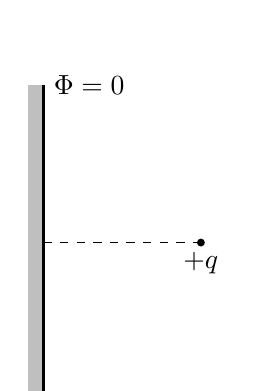
\begin{tikzpicture}
            \fill[gray!50](-.2, 0)rectangle(0, 4);%pattern=north east lines
            \draw[thick](0, 0)--(0, 4)node[right]{$\Phi=0$};
            \draw[dashed](0, 2)--(2, 2);
            \fill[black](2, 2)circle(.05)node[below]{$+q$};
        \end{tikzpicture}\qqquad
        \begin{tikzpicture}
            \draw[dashed](0, 0)--(0, 4)node[right]{$\Phi=0$};
            \draw[dashed](-2, 2)--(2, 2);
            \fill[black](2, 2)circle(.05)node[below]{$+q$};
            \fill[black](-2, 2)circle(.05)node[below]{$-q$};
        \end{tikzpicture}
        \tikzchap 电像法
    \end{center}
\end{example}
\subsubsection{球导体的电像法}
\begin{example}{接地导体球的镜像电荷}{image charge of grounded conducting sphere}
    一半径为$a$的导体球接地,球外有一电荷$q$,距球心$y>a$
    \begin{center}\usetikzlibrary{circuits.ee.IEC}
        \begin{tikzpicture}[circuit ee IEC]
            \draw[thick](0, 0)circle(1.5);
            \draw (1.2, -.9) to (2, -.9) to [ground={at end}] (2, -1.5);
            \draw[dashed](0, 0)node[left]{$O$}--(4, 0);
            \fill[black](4, 0)circle(.05)node[below]{$y$}node[above]{$q$};
        \end{tikzpicture}
        \tikzchap 接地导体球和点电荷
    \end{center}
    我们可以在球壳内放置一镜像电荷$q'$,且由对称性,镜像电荷一定在原电荷与球心的连线上:
    \begin{center}
        \begin{tikzpicture}
            \draw[dashed](0, 0)circle(1.5);
            \draw[dashed](0, 0)node[left]{$O$}--(4, 0);
            \fill[black](4, 0)circle(.05)node[below]{$y$}node[above]{$q$};
            \fill[black](.5625, 0)circle(.05)node[below]{$y'$}node[above]{$q'$};
        \end{tikzpicture}
        \tikzchap 镜像电荷
    \end{center}
    不难验证,取
    \begin{equation}
        \label{eqn:image of point, grounded conducting sphere}
        q'=-\frac ayq,\quad yy'=a^2.
    \end{equation}
    便可使原球面所在位置上的电势均为0.
    \begin{equation}
        \Phi(\bm x)=\frac q{4\pi\varepsilon_0}\biggkh{\frac1{|\bm x-\bm y|}-\frac ay\frac1{|\bm x-\bm y'|}},\quad\bm y'=\Bigkh{\frac ay}^2\bm y.
    \end{equation}
    \tcblower
    接地导体球外表面的面电荷密度为($n'$指向球内,即$-r$方向)
    \begin{equation}
        \label{eqn:surface charge density of grounded conducting sphere, point}
        \sigma=-\varepsilon_0\edg{\pv\Phi r}_{r=a}=-\frac q{4\pi a}\frac{y^2-a^2}{(y^2+a^2-2ay\cos\theta)^{3/2}}.
    \end{equation}
    球体上的总感应电荷等于像电荷$q'$。%,根据Gauss定律,这是必然的。当然我们也可以通过积分直接证明。
    作用在电荷$q$上的力%可以用不同的方法来计算。最简单的方法是计算电荷$q$和像电荷$q'$之间的Coulomb力:
    \begin{equation}
        \label{eqn:force between point, grounded conducting sphere}
        F=\frac1{4\pi\varepsilon_0}\frac{qq'}{(y-y')^2}=\frac{q^2}{4\pi\varepsilon_0}\frac{ay}{(y^2-a^2)^2}.
    \end{equation}
\end{example}
我们注意到,整个讨论都是基于点电荷在导体球外。实际上,这个结果同样适用于球内的电荷($y<a$)。唯一需要改变的是(\ref{eqn:surface charge density of grounded conducting sphere, point}),其中导体外的法向导数现在是径向向内的,这意味着符号的变化。导体球内表面感应电荷为$-q$,与$y$无关。
\begin{example}{带电孤立导体球的镜像电荷}{image charge of charged insulated conducting sphere}
    将例 \ref{exm:image charge of grounded conducting sphere} 的导体球换为总电荷为$Q$的孤立导体球,可以用线性叠加法建立电势的解:
    \begin{compactenum}
        \item 首先将导体球接地,即例 \ref{exm:image charge of grounded conducting sphere} 得到的结果;
        \item 然后切断导体球的接地,导体球外表面会带上$q'$的电荷,我们只需要再向外表面添加$(Q-q')$的电荷即可,由于导体是等电位的,这些$(Q-q')$电荷将均匀地分布在外表面上。
    \end{compactenum}
    因此电势会添加一项等效于处于原点的$(Q-q')$点电荷的电势。
    
    而原点电荷受到的力为
    \begin{equation}
        F=\frac1{4\pi\varepsilon_0}\frac q{y^2}\biggfkh{Q-q\frac{a^3(2y^2-a^2)}{y(y^2-a^2)^2}}.
    \end{equation}
    当$y\gg a$时,电场力会退化为两个点电荷之间的Coulomb力
    \[
        F\simeq\frac1{4\pi\varepsilon_0}\frac{qQ}{y^2}.
    \]
    当$Q\gg q$时,相互作为用0的点(不稳定平衡点)坐标$y$为
    \begin{equation}
        Q\simeq\frac{qa^2}{4(y-a)^2},\thus y\simeq a\biggkh{1+\frac12\sqrt{\frac qQ}}.
    \end{equation}
\end{example}
当点电荷处于导体球内时,由Gauss定律,导体球内表面会产生$-q$的感应电荷。因此若导体球带总电荷为$Q$时,其外表面电荷应为$Q+q$,且均匀地分布在外表面。
\begin{example}{固定电势导体球的镜像电荷}{image charge of conducting sphere at fixed potential}
    将例 \ref{exm:image charge of grounded conducting sphere} 的导体球换为电势为$V$的导体球,类似于例 \ref{exm:image charge of charged insulated conducting sphere},但额外加在导体球上的电荷$(Q-q')$应改为$(4\pi\varepsilon_0\cdot Va)$。
\end{example}
\begin{example}{电像法处理匀强电场中的导体球问题}{conducting sphere in uniform electric field by method of images}
    考虑均匀电场$E_0$中半径为$a$的导体球。均匀场可以认为是在无穷远处由带适当电荷的正负电荷产生的,如下图所示
    \begin{center}
        \begin{tikzpicture}
            \draw(-5, 0)--(5, 0);
            \fill[black](4, 0)circle(.05)node[above]{$-Q$}node[below]{$+R$};
            \fill[black](-4, 0)circle(.05)node[above]{$+Q$}node[below]{$-R$};
            \draw[dashed](-4, 0)--(0, .8)--(4, 0);
            %\draw[thick, latex-latex](1, 1)--(0, .8)--(1, .6);
            \draw[thick, -latex](0, .8)--(2, .8)node[above]{$\bm E_0$};
        \end{tikzpicture}
        \tikzchap{正负电荷近似匀强电场}
    \end{center}
    有两个电荷$\pm Q$,位于$\mp R$位置,在原点附近电场可以近似为均匀。
    \[
        E\simeq\frac1{4\pi\varepsilon_0}\frac{2Q}{R^2}.
    \]
    保持$Q/R^2$不变,在$R,Q\to\infty$的极限下,这个近似是精确的。

    因此使用电像法的结论,构造两个镜像电荷$\pm Qa/R$,得到球坐标系下的电势$\Phi(r,\theta)$,
    \iffalse
    \begin{align*}
        \Phi(r,\theta)=\frac1{4\pi\varepsilon_0}\Bigg[\frac{Q}{(r^2+R^2+2Rr\cos\theta)^{1/2}}-\frac{Q}{(r^2+R^2-2Rr\cos\theta)^{1/2}}\\
        -\frac{aQ}{R\biggkh{r^2+\dfrac{a^4}{R^2}+2\dfrac{a^2}Rr\cos\theta}^{1/2}}+\frac{aQ}{R\biggkh{r^2+\dfrac{a^4}{R^2}-2\dfrac{a^2}Rr\cos\theta}^{1/2}}\Bigg].
    \end{align*}
    \fi
    由于$R\gg r$,可进行Taylor展开:
    \begin{align}
        \notag
        \Phi(r,\theta)&=\frac1{4\pi\varepsilon_0}\frac{2Q}{R^2}\biggkh{-r\cos\theta+\frac{a^3}{r^2}\cos\theta+\cdots}\\
        &=-E_0\biggkh{r-\frac{a^3}{r^2}}\cos\theta.
    \end{align}
    省略号部分内容随着$R\to\infty$而消失。则导体球的面电荷密度为
    \begin{equation}
        \sigma=-\varepsilon_0\edg{\pv\Phi r}_{r=a}=3\varepsilon_0E_0\cos\theta.
    \end{equation}
    电荷密度的面积分为0,因此导体球接地与否没有区别。
\end{example}
\subsubsection{球边界的Green函数}
对于球形Dirichlet边界条件,为了使球面上的$G(\bm x,\bm x')=0$,可借助镜像电荷的思想,取
\begin{equation}
    \label{eqn:sphere Green function}
    G(\bm x,\bm x')=\frac1{|\bm x-\bm x'|}-\frac a{x'}\frac1{|\bm x-\bm x''|},\quad\bm x''=\Bigkh{\frac{a}{x'}}^2\bm x'.
\end{equation}
令$\gamma$表示$\bm x,\bm x'$夹角,则
\[
    G(\bm x,\bm x')=\frac1{(x^2+x'^2-2xx'\cos\gamma)^{1/2}}-\frac a{(x^2x'^2+a^4-2a^2xx'\cos\gamma)^{1/2}},
\]
式(\ref{eqn:Dirichlet Green})中还需要$\p G/\p n'$,若感兴趣的区域为球外,则$n'$指向球内,
\begin{equation}
    \label{eqn:sphere dGreen function}
    \edg{\pv G{n'}}_{x'=a}=-\edg{\pv G{x'}}_{x'=a}=-\frac{x^2-a^2}{a(x^2+a^2-2ax\cos\gamma)^{3/2}}.
\end{equation}
这正是式(\ref{eqn:surface charge density of grounded conducting sphere, point})的感应表面电荷密度。

由此我们得到:给定球表面电势$\Phi(a,\theta,\phi)$下,球外Laplace方程的解
\begin{equation}
    \label{eqn:sphere Laplace solution}
    \Phi(r,\theta,\phi)=\frac1{4\pi}\oint_{\p V}\Phi(a,\theta',\phi')\frac{a(r^2-a^2)}{(r^2+a^2-2ar\cos\gamma)^{3/2}}\d\Omega'
\end{equation}
$\d\Omega'=\sin\theta'\d\theta'\nd\phi'$是点$(a,\theta',\phi')$处的立体角微元,且
\[
    \cos\gamma=\cos\theta\cos\theta'+\sin\theta\sin\theta'\cos(\phi-\phi').
\]
若问题改为球内的Laplace方程,则法向量方向反向,式(\ref{eqn:sphere dGreen function})的$\p G/\p n'$结果要变号。
\begin{example}{两半球具有不同电势的导体球}{conducting sphere with hemispheres at different potentials}
    一个半径为$a$的导电球由两个电势分别为$\pm V$的半球壳组成,
    \begin{center}
        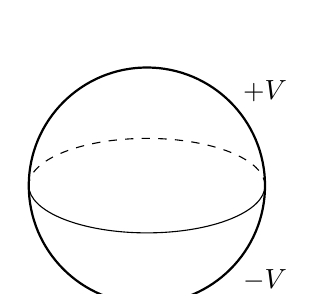
\begin{tikzpicture}[scale=.6]
            \draw[thick](0, 0)circle(2.5);
            \draw[dashed](2.5, 0)arc(0:180:2.5 and 1);
            \draw(-2.5, 0)arc(-180:0:2.5 and 1);
            \node at(2.5, 2){$+V$};
            \node at(2.5, -2){$-V$};
        \end{tikzpicture}
        \tikzchap 两半球具有不同电势的导体球
    \end{center}
    使用式(\ref{eqn:sphere Laplace solution}),
    \begin{align*}
        \Phi(\bm x)&=\frac V{4\pi}\int_0^{2\pi}\biggkh{\int_0^1-\int_{-1}^0}\frac{a(r^2-a^2)}{(r^2+a^2-2ar\cos\gamma)^{3/2}}\d(\cos\theta')\nd\phi'\\
        &=\frac{Va(r^2-a^2)}{4\pi}\int_0^{2\pi}\bs5\int_0^1\Bigl[(r^2+a^2-2ar\cos\gamma)^{-3/2}-\\
        &\qqquad(r^2+a^2+2ar\cos\gamma)^{-3/2}\Bigr]\d(\cos\theta')\nd\phi'.
    \end{align*}
    考虑$+z$轴上的电势,取$\theta=0$,则$\cos\gamma=\cos\theta'$,得到 
    \begin{equation}
        \Phi(z)=V\biggfkh{1-\frac{z^2-a^2}{z\sqrt{z^2+a^2}}}
    \end{equation}
    当$z\gg a$时,$\Phi(z)\simeq 3Va^2/2z^2$。

    为了得到上面积分的表达式,提出$(r^2+a^2)$,
    \begin{align*}
        \Phi(\bm x)&=\frac{Va(r^2-a^2)}{4\pi(r^2+a^2)^{3/2}}\int_0^{2\pi}\bs5\int_0^1\\
        &\qquad\Bigl[(1-2\alpha\cos\gamma)^{-3/2}-(1+2\alpha\cos\gamma)^{-3/2}\Bigr]\d(\cos\theta')\nd\phi'
    \end{align*}
    其中$\alpha:=ar/(a^2+r^2)$,进行Taylor展开:
    \[
        (1-2\alpha\cos\gamma)^{-3/2}-(1+2\alpha\cos\gamma)^{-3/2}=6\alpha\cos\gamma+35\alpha^3\cos^3\gamma+\cdots
    \]
    按项积分得到
    \[
        \Phi(\bm x)=\frac{3Va^2}{2r^2}\frac{r^3(r^2-a^2)}{(r^2+a^2)^{5/2}}\cos\theta\biggfkh{1+\frac{35}{24}\frac{a^2r^2}{(r^2+a^2)^2}(3-\cos^2\theta)+\cdots}.
    \]
    若$r\gg a$,则
    \begin{equation}
        \Phi(r,\theta,\phi)=\frac{3Va^2}{2r^2}\biggfkh{\cos\theta-\frac{7a^2}{12r^2}\biggkh{\frac52\cos^3\theta-\frac32\cos\theta}+\cdots}.
    \end{equation}
    对应Legendre多项式$P_1(\cos\theta),P_3(\cos\theta)$。见例 \ref{exm:conducting sphere with hemispheres at different potentials II} 续。
\end{example}
若题目变为两个$V_1,V_2$的半导体球,我们也可以写成$(V_1+V_2)/2$的完整孤立导体球与两个$\pm(V_1-V_2)/2$的半导体球的叠加。
\subsection{正交函数展开法}
\begin{definition}{正交函数}{orthogonal function}
    一组实(复)函数$U_i(\xi)$在区间$(a,b)$上平方可积,若两两正交(orthogonal):
    \begin{equation}
        \int_a^bU_m^\ast(\xi)U_n(\xi)\d\xi=\delta_{mn}.
    \end{equation}
    则称为正交函数。其中$\delta_{mn}$为Kronecker符号。
\end{definition}
若有一组完备的正交函数集$\{U_i(\xi)\}$,则在区间$(a,b)$上任意平方可积的函数$f(x)$均可被展开成正交函数的线性组合
\[
    f(\xi)=\sum_{i=1}^\infty a_iU_i(\xi),\quad a_i:=\int_a^bU_i^\ast(\xi)f(\xi)\d\xi.
\]
即
\[
    f(\xi)=\int_a^b\biggfkh{\sum_{i=1}^\infty U_i^\ast(\xi')U_i(\xi)}f(\xi')\d\xi'.
\]
易得完备(闭合)关系
\begin{equation}
    \sum_{i=1}^\infty U_i^\ast(\xi')U_i(\xi)=\delta(\xi'-\xi).
\end{equation}
\begin{example}{Fourier级数}{Fourier series}
    易证,在区间$(-\pi,\pi)$内,函数
    \[
        \{1,\sin x,\cos x,\sin 2x,\cos 2x,\ldots\}
    \]
    两两正交,归一化之
    \[
        \hkh{\frac1{\sqrt{2\pi}},\frac{\sin x}{\sqrt\pi},\frac{\cos x}{\sqrt\pi},\frac{\sin 2x}{\sqrt\pi},\frac{\cos 2x}{\sqrt\pi},\ldots}
    \]
    因此,在$(-\ell/2,\ell/2)$区间内的一组正交函数为
    \[
        \hkh{\frac1{\sqrt\ell},\ldots,\sqrt{\frac2\ell}\sin\biggkh{\frac{2\pi nx}\ell},\enspace\sqrt{\frac2\ell}\cos\biggkh{\frac{2\pi nx}\ell},\ldots}
    \]
    在$(-\ell/2,\ell/2)$上平方可积的函数$f(x)$可被展开为Fourier级数
    \begin{equation}
        f(x)=\frac{a_0}2+\sum_{n=1}^\infty\biggfkh{a_n\cos\biggkh{\frac{2\pi nx}{\ell}}+b_n\sin\biggkh{\frac{2\pi nx}{\ell}}}.
    \end{equation}
    其中Fourier系数
    \begin{align*}
        a_n&=\frac2\ell\int_{-\ell/2}^{\ell/2}f(x)\cos\biggkh{\frac{2\pi nx}{\ell}}\d x\\
        b_n&=\frac2\ell\int_{-\ell/2}^{\ell/2}f(x)\sin\biggkh{\frac{2\pi nx}{\ell}}\d x
    \end{align*}
\end{example}
一般化至二维,对于任意$(a,b)\times(c,d)$上平方可积的函数$f(\xi,\eta)$,若可在两个维度分别找到一组正交函数$U_i(\xi),V_j(\eta)$,则$f(\xi,\eta)$可被展开为
\[
    f(\xi,\eta)=\sum_{i=1}^\infty\sum_{j=1}^\infty a_{ij}U_i(\xi)V_j(\eta),
\]
其中 
\[
    a_{ij}=\int_a^b\bs3\int_c^dU_i(\xi)V_j(\eta)f(\xi,\eta)\d\eta\nd\xi
\]
\begin{example}{Fourier变换}{Fourier transformation}
    Fourier级数有复变函数的形式
    \[
        f(x)=\frac1{\sqrt\ell}\sum_{n=-\infty}^{+\infty}c_n\e{\i2\pi nx/\ell},\quad c_n=\frac1{\sqrt\ell}\int_{-\ell/2}^{\ell/2}f(x')\e{-\i2\pi nx'/\ell}\d x'.
    \]
    当$\ell\to\infty$时,
    \[
        f(x)=\frac1{2\pi}\int\iti\biggfkh{\int\iti f(x')\e{-\i kx'}\d x'}\e{\i kx}\d k.
    \]
    由此可得$f(x)$的Fourier变换为
    \begin{equation}
        \hat f(k)=\frac1{\sqrt{2\pi}}\int\iti f(x)\e{-\i kx}\d x;
    \end{equation}
    相应的Fourier反变换为
    \begin{equation}
        f(x)=\frac1{\sqrt{2\pi}}\int\iti\hat f(k)\e{\i kx}\d k.
    \end{equation}
    其体现的正交性:
    \[
        \frac1{2\pi}\int\iti\e{\i(k-k')x}\d x=\delta(k-k').
    \]
\end{example}
\subsubsection{分离变量法}
数学物理中的偏微分方程(PED)通常用分离变量的方法来求解。学过数学物理方法的人都知道,这里就不多介绍了。涉及三维Laplacian的方程已知可在11个不同的坐标系中分离\footnote{\href{https://www.researchgate.net/publication/316991519_Morse_and_Feshbach's_Methods_of_Theoretical_Physics_Vol1_Morse_and_Feshbach_1953}{Morse and Feshbach, Methods of Theoretical Physics, Vol.1}}。我们只详细讨论其中的三种:矩形、球形和圆柱形。

对于矩形边界,Laplace方程为
\[
    \lapla\Phi=\pv[2]\Phi x+\pv[2]\Phi y+\pv[2]\Phi z=0.
\]
分离变量
\[
    \Phi(x,y,z)=X(x)Y(y)Z(z),
\]
代入原方程 
\[
    \frac{X''}X+\frac{Y''}Y+\frac{Z''}Z=0.
\]
对任意的$(x,y,z)$均成立,因此
\[
    X''=-\alpha^2X,\quad Y''=-\beta^2Y,\quad Z''=\gamma^2Z.
\]
其中$\gamma^2=\alpha^2+\beta^2$,解得通解
\[
    X_\pm=\e{\pm\i\alpha x},\quad Y_\pm=\e{\pm\i\beta y},\quad Z_\pm=\e{\pm\gamma z}.
\]
\begin{example}{矩形区域边界条件下的Laplace方程的解}{solution in rectangle Laplace}
    给定边界条件,比如只有$z=c$的边界有电势$V(x,y)$外,其他面电势均为0,
    \begin{center}
        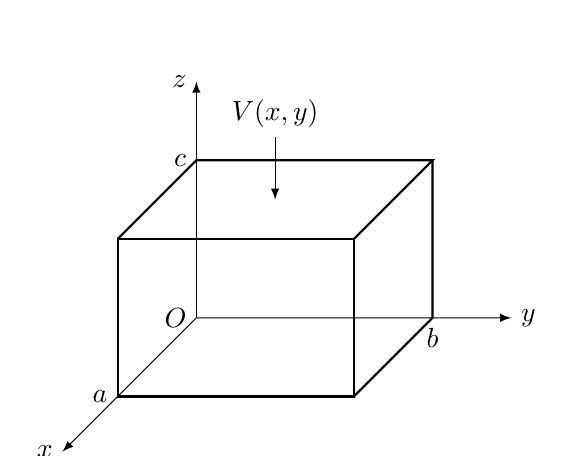
\begin{tikzpicture}
            \draw[thick](0, 0)node[left]{$a$}rectangle(3, 2);
            \draw[thick](0, 2)--(1, 3)node[left]{$c$}--(4, 3)--(3, 2);
            \draw[thick](4, 3)--(4, 1)node[below]{$b$}--(3, 0);
            \draw[latex-latex](5, 1)node[right]{$y$}--(1, 1)node[left]{$O$}--(-.7, -.7)node[left]{$x$};
            \draw[-latex](1, 1)--(1, 4)node[left]{$z$};
            \draw[-latex](2, 3.3)node[above]{$V(x,y)$}--(2, 2.5);
        \end{tikzpicture}
        \tikzchap 矩形区域边界条件
    \end{center}
    则
    \[
        X=\sin(\alpha x),\quad Y=\sin(\beta y),\quad Z=\sinh(\gamma z);
    \]
    因为$x=a,y=b$处$\Phi=0$,故应有驻波条件
    \[
        \alpha_m=\frac{m\pi}a,\quad\beta_n=\frac{n\pi}b,\quad\gamma_{mn}=\pi\sqrt{\frac{m^2}{a^2}+\frac{n^2}{b^2}}.
    \]
    $\Phi$一定可以写成满足Laplace方程的一系列正交函数的线性组合
    \[
        \Phi(x,y,z)=\sum_{m,n}A_{mn}\sin(\alpha_mx)\sin(\beta_ny)\sinh(\gamma_{mn}z).
    \]
    为满足$z=c$上的边界条件
    \[
        V(x,y)=\sum_{m,n}A_{mn}\sin(\alpha_mx)\sin(\beta_ny)\sinh(\gamma_{mn}c).
    \]
    易得系数
    \[
        A_{mn}=\frac4{ab\sinh(\gamma_{mn}c)}\int_0^a\bs3\int_0^bV(x,y)\sin(\alpha_mx)\sin(\beta_ny)\d y\nd x.
    \]
\end{example}
\subsubsection{二维边界问题}
现在我们简单地考虑二维Laplace方程在直角坐标下的分离变量解法。
\begin{example}{二维边界条件}{2D boundary condition}
    \begin{equation*}
        \begin{cases}
            \pv[2]\Phi x+\pv[2]\Phi y=0,&0<x<a,y>0\\
            \Phi(0,y)=\Phi(a,y)=0,&y>0\\
            \Phi(x, 0)=V(x),&0<x<a
        \end{cases}
    \end{equation*}
    分离变量$\Phi(x,y)=X(x)Y(y)$易得
    \[
        X_n(x)=\sin\biggkh{\frac{n\pi x}a},\quad Y_n(y)=\exp\biggkh{-\frac{n\pi y}a},\quad n=1,2,\ldots
    \]
    有形式解
    \begin{equation}
        \Phi(x,y)=\sum_{n=1}^\infty A_n\sin\biggkh{\frac{n\pi x}a}\exp\biggkh{-\frac{n\pi y}a}.
    \end{equation}
    代入边界条件
    \[
        \Phi(x,0)=\sum_{n=1}^\infty A_n\sin\biggkh{\frac{n\pi x}a}=V(x),
    \]
    得到系数
    \[
        A_n=\frac2a\int_0^aV(x)\sin\biggkh{\frac{n\pi x}a}\d x.
    \]
\end{example}
二维极坐标Laplace方程
\begin{equation}
    \frac1\rho\pp\rho\biggkh{\rho\pv\Phi\rho}+\frac1{\rho^2}\pv[2]\Phi\phi=\pv[2]\Phi\rho+\frac1\rho\pv\Phi\rho+\frac1{\rho^2}\pv[2]\Phi\phi=0.
\end{equation}
分离变量$\Phi(\rho,\phi)=R(\rho)\Psi(\phi)$,设
\[
    \begin{cases}
        \rho^2R''+\rho R'-\lambda R=0,\\
        \Psi''+\lambda\Psi=0.
    \end{cases}
\]
由周期条件
\[
    \Psi(\phi+2\pi)=\Psi(\phi),\quad\Psi'(\phi+2\pi)=\Psi'(\phi).
\]
可得$\lambda=n^2,\enspace n=0,1,2,\ldots$
\[
    \Psi(\phi)=a_n\cos n\phi+b_n\sin n\phi.
\]
$R(\rho)$满足Euler方程,做变量替换$u(t)=R(\e t)$,
\[
    u''-n^2u=0,\thus u=
    \begin{cases}
        c_0+d_0t,&n=0\\
        c_n\e{nt}+d_n\e{-nt},&n\geqslant 1
    \end{cases}
\]
可得
\[
    R(\rho)=
    \begin{cases}
        c_0+d_0\ln\rho,&n=0\\
        c_n\rho^n+d_n\rho^{-n},&n\geqslant 1
    \end{cases}
\]
故
\begin{equation}
    \Phi(\rho,\phi)=c_0+d_0\ln\rho+\sum_{n=1}^{\infty}(a_n\cos n\phi+b_n\sin n\phi)(c_n\rho^n+d_n\rho^{-n}).
\end{equation}
若区域包含原点,则要求$d_n\equiv 0$。
\begin{example}{二维拐角内和沿棱边的电场与电荷密度}{field and charge density in 2D Corners and along edges}
    \begin{center}
        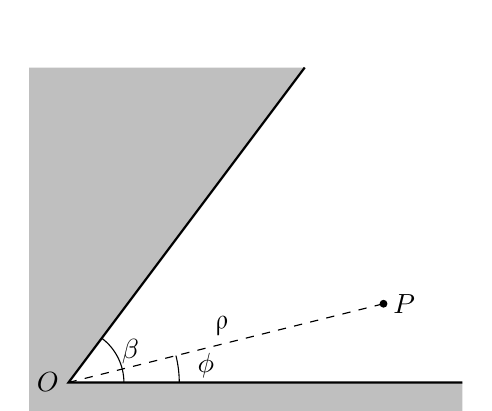
\begin{tikzpicture}
            \coordinate (o) at (0, 0);
            \coordinate (p) at (4, 1);
            \coordinate (a) at (5, 0);
            \coordinate (b) at (3, 4);
            \fill[gray!50](-.5, 4)--(b)--(o)--(a)--(5, -.5)--(-.5, -.5);
            \draw[thick](b)--(o)--(a);
            \draw[dashed](o)node[left]{$O$}--(p)node[midway, above, sloped]{$\rho$};
            \fill(p)circle(.05)node[right]{$P$};
            \pic["$\beta$", draw, angle eccentricity=1.25, angle radius=20]{angle=a--o--b};
            \pic["$\phi$", draw, angle eccentricity=1.25, angle radius=40]{angle=a--o--p};
        \end{tikzpicture}
        \tikzchap 极坐标
    \end{center}
    由边界条件,$\lambda=(n\pi/\beta)^2$,
    \begin{equation}
        \Phi(\rho,\phi)=V+\sum_{n=1}^\infty a_n\rho^{n\pi/\beta}\sin\biggkh{\frac{n\pi\phi}\beta}.
    \end{equation}
    $\rho\to0$时,忽略高阶项
    \[
        \Phi\simeq V+a_1\rho^{\pi/\beta}\sin\biggkh{\frac{\pi\phi}\beta}.
    \]
    电场 
    \begin{equation}
        \begin{cases}
            E_\rho=-\pv\Phi\rho\simeq-\frac{\pi a_1}\beta\rho^{\pi/\beta-1}\sin\biggkh{\frac{\pi\phi}\beta}.\\
            E_\phi=-\frac1\rho\pv\Phi\phi\simeq-\frac{\pi a_1}\beta\rho^{\pi/\beta-1}\cos\biggkh{\frac{\pi\phi}\beta}
        \end{cases}
    \end{equation}
    边界感应电荷密度
    \begin{equation}
        \sigma(\rho)=\varepsilon_0E_\phi(\rho,0)\simeq-\frac{\varepsilon_0\pi a_1}\beta\rho^{\pi/\beta-1}.
    \end{equation}
    当$\beta>\pi$时,$\sigma$在$\rho\to0$有奇点。这便是尖端放电现象的解释。
\end{example}
\subsectionstar{有限元分析法}
略
\paragraph{第二部分}
这一章会继续讨论静电学中的边值问题,主要内容分为四节。

前两节的内容属于属于数理方法中的常规内容,在球坐标和柱坐标中用分离变量法求解Laplace方程。注意其中扼要介绍了Legendre多项式、球谐函数、Bessel函数等特殊函数的性质。

第三节内容为在球坐标系和柱坐标系中应用Green函数法求解Poisson方程。考虑到实际问题往往带有电荷分布,故Poisson方程更为普遍。事实上Poisson方程的解,在第一章中已有所介绍,且已给出了三种边界条件(Dirichlet, Neumann, Robin)对应通解的形式,在本节会从解决具体问题的角度进一步做阐述。

第四节讨论了混合边界条件下的边值问题,并举一实例简要说明了这类问题的难点(这类问题其实往往颇为复杂……)

%值得一提的是,本章内容大多和MMP(数学物理方法,Methods of Mathematical Physics)挂钩,所以一些数学计算的过程(如特殊函数的级数表达式、收敛问题,以及各种完备性的证明等……)被我省略掉了,具体内容可以参考:
\subsection{球坐标系中的正交函数}
球坐标系$(r,\theta,\phi)$,Laplace方程可以写成
\begin{equation}
    \label{eqn:Laplace in spherical}
    \frac1{r^2}\pp r\biggkh{r^2\pv\Phi r}+\frac1{r^2\sin\theta}\pp\theta\biggkh{\sin\theta\pv\Phi\theta}+\frac1{r^2\sin^2\theta}\pv[2]\Phi\phi=0.
\end{equation}
分离变量$\Phi(r,\theta,\phi)=R(r)P(\theta)Q(\phi)$,得到 
\[
    \begin{cases}
        \dd r\biggkh{r^2\dv Rr}-\ell(\ell+1)R=0,\\
        \frac1{\sin\theta}\dd\theta\biggkh{\sin\theta\dv P\theta}+\biggfkh{\ell(\ell+1)-\frac{m^2}{\sin^2\theta}}P=0,\\
        \frac1Q\dv[2]Q\phi=-m^2.
    \end{cases}
\]
可直接解得$R,Q$
\begin{align}
    R_\ell&=Ar^\ell+Br^{-(\ell+1)},\\
    Q_m&=\e{\pm\i m\phi},\quad m=0,\pm 1,\pm 2,\ldots
\end{align}
\subsubsection{Legendre多项式}
$P(\theta)$经常通过$x=\cos\theta$代换,得到广义(generalized) Legendre方程:
\begin{equation}
    \label{eqn:general Legendre}
    \dd x\biggfkh{(1-x^2)\dv Px}+\biggfkh{\ell(\ell+1)-\frac{m^2}{1-x^2}}P=0.
\end{equation}
考虑$m=0$的情形,得到Legendre方程:
\begin{equation}
    \label{eqn:Legendre}
    \dd x\biggfkh{(1-x)^2\dv Px}+\ell(\ell+1)P=0.
\end{equation}
采用级数解,设
\[
    P(x)=x^\alpha\sum\fmto j0 a_jx^j.
\]
$\alpha$是待定系数,从而 
\[
    \sum\fmto j0(\alpha+j)(\alpha+j-1)a_j x^{\alpha+j-2}-\sum\fmto j0\bigfkh{(\alpha+j)(\alpha+j+1)-\ell(\ell+1)}a_jx_{\alpha+j}=0.
\]
解得
\[
    \begin{cases}
        a_0\alpha(\alpha-1)=0,&j=0\\
        a_1\alpha(\alpha+1)=0,&j=1\\
        a_{j+2}=\frac{(\alpha+j)(\alpha+j+1)-\ell(\ell+1)}{(\alpha+j+1)(\alpha+j+2)}a_j,&j\geqslant 0
    \end{cases}
\]
初始条件中有多种可能的情况:
\begin{compactitem}
	\item $a_0=a_1=0$,解$P\equiv 0$是平凡的;
	\item $a_0=0,\enspace a_1\neq 0$,展开式事实上与$a_0\neq 0,\enspace a_1=0$等价:
	\[
        P(x)=x^\alpha(a_1x+a_3x^3+\cdots)=x^{\alpha+1}(a_1+a_3x^2+\cdots);
    \]
	\item $a_0\neq 0,\enspace a_1\neq 0$,由递推关系知,级数会在$x=\pm 1$发散。
\end{compactitem}
综上,我们最终选取$a_0\neq 0,\enspace a_1=0$,从而$\alpha(\alpha-1)=0$,
\[
    P(x)=\begin{cases}
        a_0+a_2x^2+a_4x^4+\cdots,&\alpha=0\\
        a_0x+a_2x^3+a_4x^5+\cdots,&\alpha=1
    \end{cases}
\]
这个级数在$|x|<1$时当然收敛,但在$x=\pm 1$时会发散,除非级数在某一处终止(即之后的系数均为0)。考察递推关系:
\[
    a_{j+2}=\begin{cases}
        \frac{j(j+1)-\ell(\ell+1)}{(j+1)(j+2)}a_j,&\alpha=0\\[2ex]
        \frac{(j+1)(j+2)-\ell(\ell+1)}{(j+2)(j+3)}a_j,&\alpha=1
    \end{cases}
\]
因此,$\ell=0,1,2,\ldots$
\begin{example}{前几个Legendre多项式}{first few Legendre polynomial}
    \begin{center}
        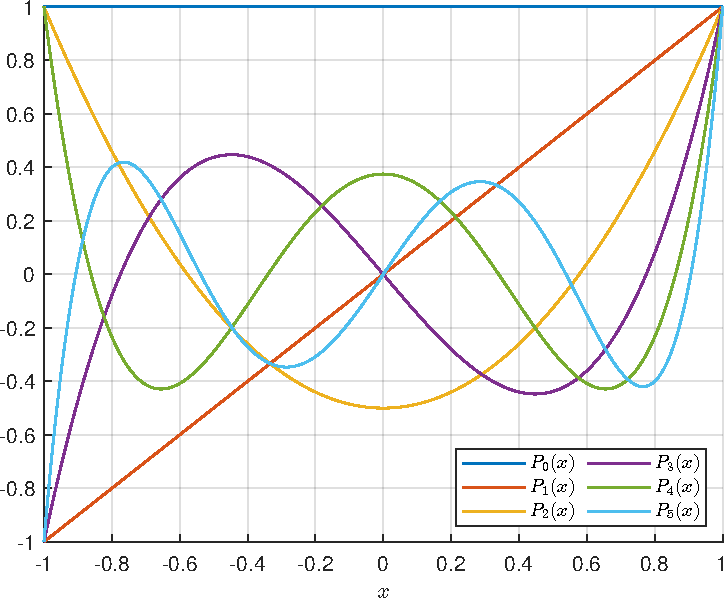
\includegraphics[width=7cm]{graphs/Legendre.pdf}
        \tikzchap 前几个Legendre多项式
        \begin{align*}
            P_0&=1,&P_2&=\frac12(3x^2-1),&P_4&=\frac18(35x^4-30x^2+3),\\
            P_1&=x,&P_3&=\frac12(5x^3-3x),&P_5&=\frac18(63x^5-70x^3+15x).
        \end{align*}
    \end{center}
\end{example}
\begin{theorem}{Rodrigues公式}{Rodrigues' formula}
    Legendre多项式可被表示为
    \begin{equation}
        \label{eqn:Rodrigues}
        P_\ell(x)=\frac1{2^\ell\ell!}\dd[\ell]x(x^2-1)^\ell.
    \end{equation}
\end{theorem}
Legendre多项式是正交的
\[
    \int_{-1}^1P_\ell(x)P_{\ell'}(x)\d x=\frac2{2\ell+1}\vd_{\ell\ell'}.
\]
因此任意$[-1,1]$上的函数均可被展开为Legendre级数
\[
    f(x)=\sum\fmto{\ell}0 A_\ell P_\ell(x),\quad A_\ell=\frac{2\ell+1}2\int_{-1}^1f(x)P_\ell(x)\d x.
\]
\begin{theorem}{Legendre多项式的递推关系}{recurrence relation among Legendre polynomial}
    可直接从Rodrigues公式和Legendre方程得到:
    \begin{gather}
        \label{eqn:Legendre 1 recurrence}
        P'_{\ell+1}-P'_{\ell-1}-(2\ell+1)P_\ell=0,\\
        (\ell+1)P_{\ell+1}-(2\ell+1)xP_\ell+\ell P_{\ell+1}=0,\\
        \notag
        P'_{\ell+1}-xP'_\ell-\ell(\ell+1)P_\ell=0,\\
        \notag
        (x^2-1)P'_\ell-\ell xP_\ell+\ell P_{\ell-1}=0.
    \end{gather}
\end{theorem}
综上,对于方位角$\phi$对称的Laplace方程(\ref{eqn:Laplace in spherical}),$m=0$,其解为
\begin{equation}
    \label{eqn:Phi(r, theta)}
    \Phi(r,\theta)=\sum\fmto{\ell}0\bigfkh{A_\ell r^\ell+B_\ell r^{-(\ell+1)}}P_\ell(\cos\theta).
\end{equation}
若区域包含原点,则要求$B_\ell\equiv 0$。
\begin{example}{两半球具有不同电势的导体球(续)}{conducting sphere with hemispheres at different potentials II}
    接例 \ref{exm:conducting sphere with hemispheres at different potentials},边界条件为
    \[
        \Phi(a,\theta)=V(\theta)=
        \begin{cases}
            +V,&0\leqslant\theta<\pi/2\\
            -V,&\pi/2<\theta\leqslant\pi
        \end{cases}
    \]
    系数满足
    \[
        A_\ell a^\ell=\frac{2\ell+1}2\int_0^\pi V(\theta)P_\ell(\cos\theta)\sin\theta\d\theta
    \]
    得$r<a$时,
    \[
        \Phi=V\biggfkh{\frac32\frac raP_1(\cos\theta)-\frac78\Bigkh{\frac ra}^3P_3(\cos\theta)+\frac{11}{16}\Bigkh{\frac ra}^5P_5(\cos\theta)+\cdots}.
    \]
    \tcblower
    球外电势,$r>a$,$A_\ell\equiv 0$。只需将$(r/a)^\ell$替换为$(a/r)^{\ell+1}$即可。
\end{example}
由于注意到$z$轴上$\theta=0,\enspace P_\ell(\cos\theta)=1$,因此另一种求解方法是先求出$z$轴上的电势,再在级数的项中添加对应的$P_\ell(\cos\theta)$。
\begin{example}{点电荷电势}{point charge potential}
    $\bm x'$处的单位点电荷在$\bm x$的产生的电势为
    \begin{equation}
        \label{eqn:1/|x-x'|}
        \frac1{|\bm x-\bm x'|}=\frac1{r_>}\sum\fmto{\ell}0\biggkh{\frac{r_<}{r_>}}^\ell P_\ell(\cos\gamma).
    \end{equation}
    其中$r_<:=\min(x,x'),\enspace r_>:=\max(x,x')$,$\gamma$是$\bm x,\bm x'$夹角。
\end{example}
\begin{example}{锥形孔内尖端附近的电场特性}{field in a conical hole or near a sharp point}
    \begin{center}
        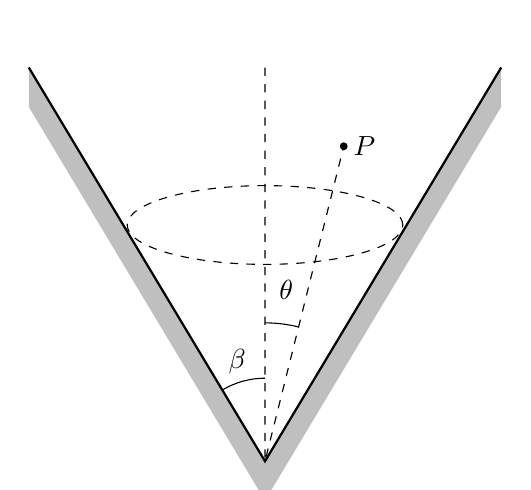
\begin{tikzpicture}
            \coordinate (o) at (0, 0);
            \coordinate (z) at (0, 5);
            \coordinate (a) at (3, 5);
            \coordinate (b) at (-3, 5);
            \coordinate (p) at (1, 4);
            \fill[gray!50](b)--(o)--(a)--(3, 4.5)--(0, -.5)--(-3, 4.5);
            \draw[thick](a)--(o)--(b);
            \draw[dashed](z)--(o)--(p);
            \draw[dashed](0, 3)ellipse(1.75 and .5);
            \fill(p)circle(.05)node[right]{$P$};
            \pic["$\beta$", draw, angle eccentricity=1.25, angle radius=30]{angle=z--o--b};
            \pic["$\theta$", draw, angle eccentricity=1.25, angle radius=50]{angle=p--o--z};
        \end{tikzpicture}
        \tikzchap 锥形孔
    \end{center}
    在$\theta=0$附近展开,设$\xi:=(1-\cos\theta)/2$,则 
    \[
        \dd\xi\biggfkh{\xi(1-\xi)\dv P\xi}+\nu(\nu+1)P=0.
    \]
    设级数解,有
    \[
        a_{j+1}=\frac{(j-\nu)(j+\nu+1)}{(j+1)^2}a_j.
    \]
    得到Legendre函数的一般表达式,这是Legendre多项式的推广
    \[
        P_\nu(\xi)=1+(-\nu)(\nu+1)\xi+\frac{(-\nu)(-\nu+1)(\nu+1)(\nu+2)}{(2!)^2}\xi^2+\cdots.
    \]
    形式解
    \[
        \Phi=Ar^\nu P_\nu(\cos\theta).
    \]
    边界条件$P_\nu(\cos\beta)=0$,可解得$\nu=\nu_k,\enspace k=1,2,\ldots$
    \[
        \Phi(r,\theta)=\sum_{k=1}^\infty A_kr^{\nu_k}P_{\nu_k}(\cos\theta).
    \]
    $r\to 0$时,考虑第一项$\Phi\simeq Ar^\nu P_\nu(\cos\theta)$,电场
    \[
        \begin{cases}
            E_r=-\pv\Phi r\simeq-\nu Ar^{\nu-1}P_\nu(\cos\theta),\\[1ex]
            E_\theta=-\frac1r\pv\Phi\theta\simeq Ar^{\nu-1}\sin\theta P'_\nu(\cos\theta).
        \end{cases}
    \]
    表面电荷密度
    \[
        \sigma_r=-\varepsilon_0E_\theta|_{\theta=\beta}\simeq-\varepsilon_0Ar^{\nu-1}\sin\beta P_\nu'(\cos\beta).
    \]
\end{example}
\subsubsection{连带Legendre函数、球谐函数}
考虑式(\ref{eqn:general Legendre}) $m\neq 0$的情形,为了使解在$[-1,1]$收敛,$\ell=0,1,2,\ldots$且$m=-\ell,-\ell+1,\ldots,\ell$,略去推导过程,解是连带(associated) Legendre函数$P_\ell^m(\cos\theta)$,与Legendre多项式的关系为: 
\[
    P_\ell^m(x)=(-)^m(1-x^2)^{m/2}\dd[m]xP_\ell(x),\quad m\geqslant 0.
\]
$P_\ell^{-m}$和$P_\ell^m$是线性相关的:
\[
    P_\ell^{-m}(x)=(-)^m\frac{(\ell-m)!}{(\ell+m)!}P_\ell^m(x).
\]
有正交关系:
\begin{align*}
    \int_{-1}^1P_\ell^m(x)P_{\ell'}^m(x)\d x&=\frac2{2\ell+1}\frac{(\ell-m)!}{(\ell+m)!}\vd_{\ell\ell'};\\
    \int_{-1}^1P_\ell^m(x)P_\ell^{m'}(x)\frac{\d x}{1-x^2}&=\frac1m\frac{(\ell+m)!}{(\ell-m)!}\vd_{mm'}.
\end{align*}
由此得到球谐函数(spherical harmonics fucntion):
\begin{equation}
    Y_{\ell m}(\theta,\phi)=\sqrt{\frac{2\ell+1}{4\pi}\frac{(\ell-m)!}{(\ell+m)!}}P_\ell^m(\cos\theta)\e{\i m\phi}.
\end{equation}
满足方程
\[
    \frac1{\sin\theta}\pp\theta\biggkh{\sin\theta\pv Y\theta}+\frac1{\sin^2\theta}\pv[2]Y\phi+\ell(\ell+1)Y=0,
\]
球谐函数自然是正交函数:
\[
    \oint Y_{\ell m}^\ast Y_{\ell'm'}\d\Omega=\int_0^{2\pi}\bs5\int_0^\pi Y_{\ell m}^\ast(\theta,\phi) Y_{\ell'm'}(\theta,\phi)\sin\theta\d\theta\nd\phi=\delta_{\ell\ell'}\vd_{mm'}.
\]
这样我们便得到了球坐标系下Laplace方程(\ref{eqn:Laplace in spherical})的通解
\begin{equation}
    \Phi(r,\theta,\phi)=\sum\fmto{\ell}0\sum_{m=-\ell}^\ell\bigfkh{A_{\ell m}r^\ell+B_{\ell m}r^{-(\ell+1)}}Y_{\ell m}(\theta,\phi).
\end{equation}
由$P_\ell(\cos\gamma)$的球谐函数展开式及(\ref{eqn:1/|x-x'|}),点电荷之间电势的球谐函数展开
\begin{equation}
    \label{eqn:1/|x-x'|=YY}
    \frac1{|\bm x-\bm x'|}=\frac{4\pi}{r_>}\sum\fmto{\ell}0\biggfkh{\frac1{2\ell+1}\biggkh{\frac{r_<}{r_>}}^\ell\cdot\sum_{m=-\ell}^\ell Y^\ast_{\ell m}(\theta',\phi')Y_{\ell m}(\theta,\phi)}.
\end{equation}
\subsection{柱坐标系中的正交函数}
柱坐标系$(\rho,\phi,z)$,Laplace方程可以写成
\begin{equation}
    \label{eqn:Laplace in cylinder}
    \frac1\rho\pp\rho\biggkh{\rho\pv\Phi\rho}+\frac1{\rho^2}\pv[2]\Phi\phi+\pv[2]\Phi z=0.
\end{equation}
分离变量$\Phi(\rho,\phi,z)=R(\rho)Q(\phi)Z(z)$,得到 
\[
    \begin{cases}
        \dv[2]R\rho+\frac1\rho\dv R\rho+\biggkh{k^2-\frac{\nu^2}{\rho^2}}R=0,\\[1ex]
        \dv[2]Q\phi+\nu^2Q=0,\\[1ex]
        \dv[2]Zz-k^2Z=0.
    \end{cases}
\]
可直接解得$Q,Z$
\begin{alignat}{2}
    Q_\nu&=\e{\pm\i\nu\phi},\quad&\nu&=0,\pm 1,\pm 2,\ldots\\
    Z_k&=\e{\pm kz},&k&>0
\end{alignat}
\subsubsection{Bessel函数}
设$x=k\rho$,得到Bessel方程
\begin{equation}
    \label{eqn:Bessel eqn}
    \dv[2]Rx+\frac1x\dv Rx+\biggkh{1-\frac{\nu^2}{x^2}}R=0.
\end{equation}
采用级数解,设 
\[
    R(x)=x^\alpha\sum\fmto j0 a_jx^j.
\]
解得
\[
    \begin{cases}
        \alpha^2=\nu^2,&j=0\\
        a_1\bigfkh{(\alpha+1)^2-\nu^2}=0,&j=1\\
        a_{j-2}=\bigfkh{\nu^2-(j+\alpha)^2}a_j,&j\geqslant 2
    \end{cases}
\]
故$\alpha=\pm\nu,\enspace a_1=0$,从而
\[
    a_{2j}=-\frac1{4j(j+\alpha)}a_{2j-2},\quad j=1,2,\ldots
\]
选取\footnote{$\nu$可以不是整数,此时阶乘$\nu!$推广为$\Gamma(\nu+1)$。}
\[
    \alpha=\nu,\enspace a_0=\frac1{2^\nu\nu!}.
\]
解得(第一类) Bessel函数
\begin{equation}
    J_\nu(x)=\sum\fmto j0\frac{(-)^j}{j!(j+\nu)!}\Bigkh{\frac x2}^{2j+\nu},
\end{equation}
当$\nu$不为整数时,$J_{-\nu}$和$J_\nu$是线性无关的,可作为Bessel方程的解系;但当$\nu$为整数时,二者线性相关:
\[
    J_{-\nu}(x)=(-)^\nu J_\nu(x),
\]
为了得到线性无关的另一解,定义Neumann函数(第二类Bessel函数)
\begin{equation}
    Y_\nu(x):=\frac{J_\nu(x)\cos(\nu\pi)-J_{-\nu}(x)}{\sin(\nu\pi)}.
\end{equation}
$J_\nu,Y_\nu$线性无关;
\begin{center}
    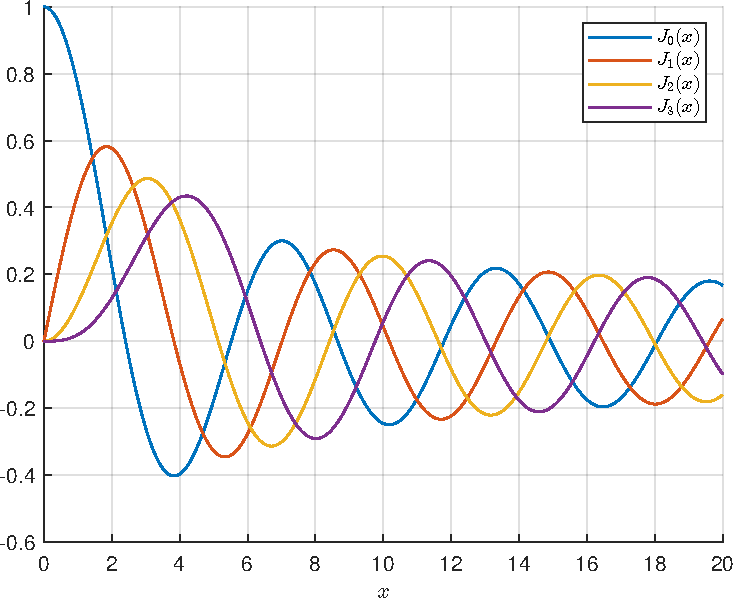
\includegraphics[width=7cm]{graphs/BesselJ.pdf}
    \tikzchap 前几个第一类Bessel函数\\[1ex]
    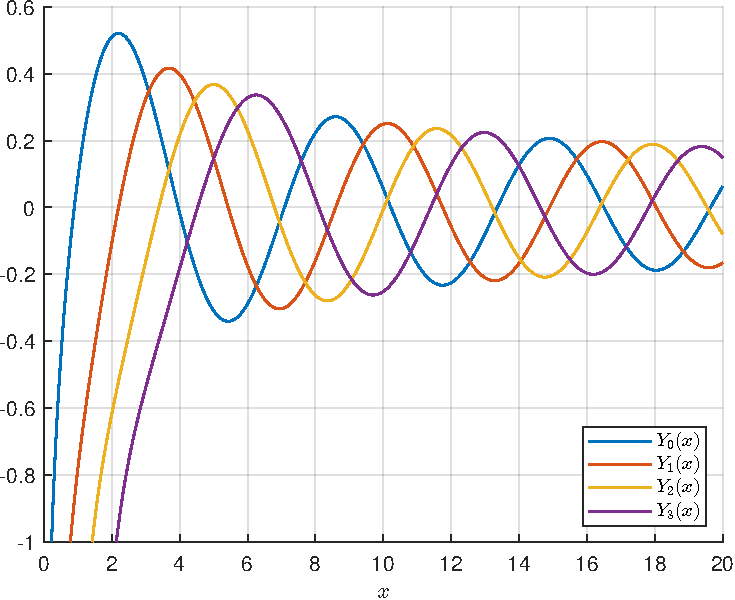
\includegraphics[width=7cm]{graphs/BesselY.pdf}
    \tikzchap 前几个第二类Bessel函数
\end{center}
Bessel方程的另一对重要线性无关解是Hankel函数(第三类Bessel函数)
\begin{equation}
    H_\nu^\pm(x)=J_\nu(x)\pm\i Y_\nu(x).
\end{equation}
三类Bessel函数均满足形如下面的递推公式
\begin{align*}
    \Omega_{\nu-1}+\Omega_{\nu+1}&=\frac{2\nu}x\Omega_\nu,\\
    \Omega_{\nu-1}-\Omega_{\nu+1}&=2\Omega'_\nu.
\end{align*}
\begin{example}{Bessel函数的渐进性}{limiting forms of Bessel function}
    $x\to 0$时, 
    \begin{align*}
        J_\nu(x)&\simeq\frac1{\nu!}\Bigkh{\frac x2}^\nu,\quad\\
        Y_\nu(x)&\simeq
        \begin{cases}
            \frac2\pi\Bigfkh{\ln\Bigkh{\frac x2}+\gamma},&\nu=0\\[1ex]
            -\frac{(\nu-1)!}\pi\Bigkh{\frac x2}^{-\nu}+\frac{\cot(\nu\pi)}{\nu!}\Bigkh{\frac x2}^\nu,&\nu\neq 0
        \end{cases}
    \end{align*}
    $\gamma$是Euler-Mascheroni常数
    \[
        \gamma:=\lim_{n\to\infty}\biggkh{-\ln n+\sum\fmto k1\frac1k}=\num{0.5772156649}.
    \]
    $x\to\infty$时, 
    \begin{align*}
        J_\nu(x)&\simeq\sqrt{\frac2{\pi x}}\cos\biggkh{x-\frac{\nu\pi}2-\frac\pi{4}},\\
        Y_\nu(x)&\simeq\sqrt{\frac2{\pi x}}\sin\biggkh{x-\frac{\nu\pi}2-\frac\pi{4}}.
    \end{align*}
\end{example}
若将$k$替换为$\i k$,便会得到修正(modified) Bessel方程
\[
    \dv[2]Rx+\frac1x\dv Rx-\biggkh{1+\frac{\nu^2}{x^2}}R=0.
\]
修正Bessel函数只是纯虚数参数的Bessel函数
\[
    I_\nu(x)=\i^{-\nu}J_\nu(\i x),\quad K_\nu(x)=\i^{\nu+1}\frac\pi 2H_\nu^+(\i x).
\]
\begin{theorem}{}{}
    $x_{\nu n}$是$J_\nu(x)$的第$n$个零点,则
    \begin{equation}
        \int_0^a J_\nu\Bigkh{x_{\nu n}\frac\rho a}J_\nu\Bigkh{x_{\nu n'}\frac\rho a}\rho\d\rho=\frac{a^2}2J_{\nu+1}^2(x_{\nu n})\vd_{nn'}.
    \end{equation}
\end{theorem}
%\prf $n\neq n'$时,由正交条件知,积分为0;$n=n'$证明略。\qed

因此$[0,a]$上的函数$f(\rho)$均可被展开为Bessel级数
\[
    f(\rho)=\sum_{n=1}^\infty A_{\nu n}J_\nu\biggkh{x_{\nu n}\frac\rho a},
\]
系数 
\[
    A_{\nu n}=\frac2{a^2J_{\nu+1}^2(x_{\nu n})}\int_0^af(\rho)J_\nu\biggkh{x_{\nu n}\frac\rho a}\rho\d\rho.
\]
\begin{example}{圆柱体内电势分布}{potential inside cylinder}
    如下图,圆柱体除顶面外其余面电势均为0.
    \begin{center}
        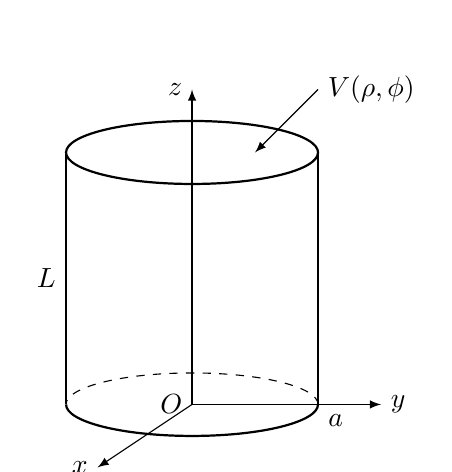
\begin{tikzpicture}[scale=.8]
            \draw[latex-latex](0, 5)node[left]{$z$}--(0, 0)node[left]{$O$}--(3, 0)node[right]{$y$};
            \draw[-latex](0, 0)--(-1.5, -1)node[left]{$x$};
            \draw[dashed](2, 0)arc(0:180:2 and .5);
            \draw[thick](-2, 0)arc(-180:0:2 and .5);
            \draw[thick](0, 4)ellipse(2 and .5);
            \draw[thick](2, 0)node[below right]{$a$}--(2, 4);
            \draw[thick](-2, 0)--(-2, 4)node[midway, left]{$L$};
            \draw[latex-](1, 4)--(2, 5)node[right]{$V(\rho,\phi)$};
        \end{tikzpicture}
        \tikzchap 圆柱形边界条件
    \end{center}
    由边界条件可知,
    \iffalse :
    \begin{align*}
        Q(\phi)&=A\sin m\phi+B\cos m\phi,\\
        Z(z)&=\sinh kz.
    \end{align*}
    \fi
    电势有形式解
    \[
        \Phi(\rho,\phi,z)=\sum_{m=0}^\infty\sum_{n=1}^\infty J_m(k_{mn}\rho)\sinh(k_{mn}z)(A_{mn}\sin m\phi+B_{mn}\cos m\phi).
    \]
    $z=L$处边界条件$\Phi(\rho,\phi,L)=V(\rho,\phi)$,可得系数
    \[
        \begin{cases}
            A_{mn}=\frac{2\csch(k_{mn}L)}{\pi a^2J_{m+1}^2(k_{mn}a)}\int_0^{2\pi}\bs5\int_0^aV(\rho,\phi)J_m(k_{mn}\rho)\sin(m\phi)\rho\d\rho\nd\phi\\
            B_{mn}=\frac{2\csch(k_{mn}L)}{\pi a^2J_{m+1}^2(k_{mn}a)}\int_0^{2\pi}\bs5\int_0^aV(\rho,\phi)J_m(k_{mn}\rho)\cos(m\phi)\rho\d\rho\nd\phi
        \end{cases}
    \]
\end{example}
\subsection{Green函数法解Poisson方程}
在 \ref{sssec:Green solve Poisson} 节中,我们介绍了Green函数方法。对于三种不同边界条件下的Poisson方程,我们给出了(\ref{eqn:Dirichlet Green})和(\ref{eqn:Neumann Green})的通解形式。在本章前面,我们用正交函数解了球坐标和柱坐标下的Laplace方程。在本节中,我们将重点讨论使用Green函数求解带有Dirichlet边界的Poisson方程。

由式(\ref{eqn:Dirichlet Green}),带Dirichlet边界条件的Poisson方程的形式解为:
\[
    \Phi(\bm x)=\frac1{4\pi\varepsilon_0}\int_V\rho(\bm x')G(\bm x,\bm x')\d v'-\frac1{4\pi}\oint_{\p V}\Phi(\bm x')\pv G{n'}\d a';
\]
因此有必要确定满足边界条件的Green函数$G(\bm x,\bm x')$。
\subsubsection{球坐标系下Green函数的展开}
对于球面边界条件,我们通常选择球坐标。然后,将Green函数表示为与所讨论的坐标相适应的函数的一系列乘积就很方便了。

事实上,根据我们所介绍的,我们可以简单地得到球坐标下Green函数的展开式。由式(\ref{eqn:1/|x-x'|=YY}),
\[
    \frac1{|\bm x-\bm x'|}=4\pi\sum\fmto{\ell}0\biggfkh{\frac1{2\ell+1}\frac{r_<^\ell}{r_>^{\ell+1}}\cdot\sum_{m=-\ell}^\ell Y^\ast_{\ell m}(\theta',\phi')Y_{\ell m}(\theta,\phi)}.
\]
我们希望得到适用于在$r = a$处具有球面边界的外部问题的Green函数的类似展开。结果很容易从(\ref{eqn:sphere Green function})中找到。
\[
    G(\bm x,\bm x')=\frac1{|\bm x-\bm x'|}-\frac a{x'}\frac1{|\bm x-\bm x''|},\quad\bm x''=\Bigkh{\frac{a}{x'}}^2\bm x'.
\]
对式(\ref{eqn:sphere Green function})中的两项展开(\ref{eqn:1/|x-x'|=YY}),得到
\begin{equation}
    \label{eqn:Green YY}
    G(\bm x,\bm x')=4\pi\sum\fmto{\ell}0\biggfkh{\frac1{2\ell+1}\frac1{r_>^{\ell+1}}\biggkh{r_<^\ell-\frac{a^{2\ell+1}}{r_<^{\ell+1}}}\sum_{m=-\ell}^\ell Y_{\ell m}^\ast(\theta',\phi')Y_{\ell m}(\theta,\phi)}.
\end{equation}
其中$r_>=\max(r,r'),\enspace r_<=\min(r,r')$。%,展开可得
\iffalse
\[
    \frac{r_<^\ell}{r_>^{\ell+1}}-\frac1a\biggkh{\frac{a^2}{rr'}}^{\ell+1}=
    \frac1{r_>^{\ell+1}}\biggkh{r_<^\ell-\frac{a^{2\ell+1}}{r_<^{\ell+1}}}
    \begin{cases}
        \frac1{r'^{\ell+1}}\biggkh{r^\ell-\frac{a^{2\ell+1}}{r^{\ell+1}}},&r<r'\\
        \biggkh{r'^\ell-\frac{a^{2\ell+1}}{r'^{\ell+1}}}\frac1{r^{\ell+1}},&r>r'
    \end{cases}
\]
\fi
\paragraph{一般展开式}
现在我们从基本原理开始,来系统地构建这种展开。有%Dirichlet势问题的Green函数满足:
\[
    \lapla G(\bm x,\bm x')=-4\pi\vd(\bm x,\bm x').
\]
且$G(\bm x,\bm x')|_{\p V}=0$。

对于球坐标,$\delta$函数可以写成
\begin{align*}
    \delta(\bm x,\bm x')&=\frac1{r^2}\vd(r-r')\vd(\phi-\phi')\vd(\cos\theta-\cos\theta')\\
    &=\frac1{r^2}\vd(r-r')\sum\fmto{\ell}0\sum_{m=-\ell}^\ell Y_{\ell m}^\ast(\theta',\phi')Y_{\ell m}(\theta,\phi).
\end{align*}
将Green函数看做$\bm x$的函数,可以被展开为
\[
    G(\bm x,\bm x')=\sum\fmto{\ell}0\sum_{m=-\ell}^\ell A_{\ell m}(r|r',\theta',\phi')Y_{\ell m}(\theta,\phi).
\]
由上面三式,可得 
\[
    A_{\ell m}(r|r',\theta',\phi')=g_\ell(r,r')Y_{\ell m}^\ast(\theta',\phi')
\]
$g_\ell$满足
\[
    \frac1r\dd[2]r\bigkh{rg_\ell(r,r')}-\frac{\ell(\ell+1)}{r^2}g_\ell(r,r')=-\frac{4\pi}{r^2}\vd(r-r').
\]
当$r\neq r'$,右边$\delta(r-r')=0$,$g_\ell$可被写成
\[
    g_\ell(r,r')=
    \begin{cases}
        Ar^\ell+Br^{-(\ell+1)},&r<r'\\
        A'r^\ell+B'r^{-(\ell+1)},&r>r'\\
    \end{cases}
\]
下一步是确定各项的系数。
\begin{example}{同心球边界条件}{concentric spheres boundary}
    设边界面为半径为$a,b\,(a<b)$的同心球面,则
    \[
        g_\ell(a,r')=0,\quad g_\ell(b,r')=0.
    \]
    可得
    \[
        g_\ell(r,r')=
        \begin{cases}
            A\biggkh{r^\ell-\frac{a^{2\ell+1}}{r^{\ell+1}}},&r<r'\\
            B'\biggkh{\frac1{r^{\ell+1}}-\frac{r^\ell}{b^{2\ell+1}}},&r>r'\\
        \end{cases}
    \]
    由于$r,r'$的对称性,$g_\ell(r,r')$可被写成 
    \[
        g_\ell(r,r')=C\biggkh{r_<^\ell-\frac{a^{2\ell+1}}{r_<^{\ell+1}}}\biggkh{\frac1{r_>^{\ell+1}}-\frac{r_>^\ell}{b^{2\ell+1}}}
    \]
    为了确定系数$C$,对$\epsilon\to0$
    \[
        \int_{r'-\epsilon}^{r'+\epsilon}\biggfkh{\dd[2]r\bigkh{rg_\ell(r,r')}-\frac{\ell(\ell+1)}{r}g_\ell(r,r')}\d r=\int_{r'-\epsilon}^{r'+\epsilon}-\frac{4\pi}r\vd(r-r')\d r.
    \]
    即
    \[
        \edg{\dd r\bigkh{rg_\ell(r,r')}}_{r'+\epsilon}-\edg{\dd r\bigkh{rg_\ell(r,r')}}_{r'-\epsilon}=-\frac{4\pi}{r'}.
    \]
    这说明$rg_\ell(r,r')$的导数在$r'$处不连续。由此
    \[
        C=\frac{4\pi}{(2\ell+1)\bigfkh{1-(a/b)^{2\ell+1}}}.
    \]
    故Green函数的展开
    \begin{equation}
        \begin{aligned}
            &G(\bm x,\bm x')=\\
            &4\pi\sum\fmto{\ell}0\sum_{m=-\ell}^\ell \frac{Y_{\ell m}^\ast(\theta',\phi')Y_{\ell m}(\theta,\phi)}{(2\ell+1)\bigfkh{1-(a/b)^{2\ell+1}}}\biggkh{r_<^\ell-\frac{a^{2\ell+1}}{r_<^{\ell+1}}}\biggkh{\frac1{r_>^{\ell+1}}-\frac{r_>^\ell}{b^{2\ell+1}}}.
        \end{aligned}
    \end{equation}
    \tcblower
    $a\to0,\,b\to\infty$时,变为式(\ref{eqn:1/|x-x'|=YY})

    $b\to\infty$时,变为式(\ref{eqn:Green YY})

    $a\to0$时,变为球内Green函数表达式。
\end{example}
\begin{example}{接地球内带电圆环}{charged ring inside grounded sphere}
    一个半径为$b$的空心接地球,其同心环的电荷半径为$a$,总电荷为$Q$,
    \iffalse
    如图所示。
    \begin{center}
        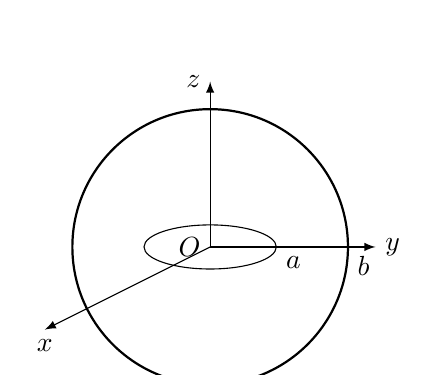
\begin{tikzpicture}[scale=.7]
            \draw[latex-latex](0, 3)node[left]{$z$}--(0, 0)node[left]{$O$}--(3, 0)node[right]{$y$};
            \draw[-latex](0, 0)--(-3, -1.5)node[below]{$x$};
            \draw[thick](0, 0)circle(2.5);
            \node[below right]at(2.5, 0){$b$};
            \draw(0, 0)ellipse(1.2 and .4);
            \node[below right]at(1.2, 0){$a$};
        \end{tikzpicture}
        \tikzchap 接地球内带电圆环
    \end{center}
    \fi
    环的电荷密度可以写成
    \[
        \rho(\bm x')=\frac Q{2\pi a^2}\vd(r'-a)\vd(\cos\theta').
    \]
    由方位角的对称性,$m=0$,故
    \begin{align*}
        \Phi(\bm x)&=\frac1{4\pi\varepsilon_0}\int\rho(\bm x')G(\bm x,\bm x')\d v'\\
        &=\frac Q{4\pi\varepsilon_0}\sum\fmto{\ell}0\biggkh{\frac{r_<^\ell}{r_>^{\ell+1}}-\frac{r^\ell a^\ell}{b^{2\ell+1}}}P_\ell(\cos\theta)P_\ell(0)\\
        &=\frac Q{4\pi\varepsilon_0}\sum_{n=0}^\infty\frac{(-)^n(2n-1)!!}{(2n)!!}\biggkh{\frac{r_<^{2n}}{r_>^{2n+1}}-\frac{r^{2n}a^{2n}}{b^{4n+1}}}P_{2n}(\cos\theta).
    \end{align*}
\end{example}
\subsubsection{柱坐标系下Green函数的展开}
柱坐标系下,
\[
    \lapla G(\bm x,\bm x')=-\frac{4\pi}\rho\vd(\rho-\rho')\vd(\phi-\phi')\vd(z-z').
\]
Green函数可以写成
\[
    G(\bm x,\bm x')=\frac1{4\pi^2}\sum_{m=-\infty}^\infty\int\iti\e{\i m(\phi-\phi')}\e{\i k(z-z')}g_m(k,\rho,\rho')\d k.
\]
径向Green函数$g_m(k,\rho,\rho')$
\begin{equation} 
    \label{eqn:cylinder green}
    \frac1\rho\dd\rho\biggkh{\rho\dv{g_m}\rho}-\biggkh{k^2+\frac{m^2}{\rho^2}}g_m=-\frac{4\pi}\rho\vd(\rho-\rho').
\end{equation}
当$\rho\neq\rho'$时,上式为修正Bessel方程,解为$I_m(k\rho),\,K_m(k\rho)$,由对称性
\[
    g_m(k,\rho,\rho')=\psi_1(k\rho_<)\psi_2(k\rho_>).
\]
$\psi_1,\psi_2$是$I_m,K_m$的线性组合。由方程右边$\delta$函数所隐含的斜率不连续条件:
\[
    \edg{\dv{g_m}\rho}_{\rho'+\epsilon}-\edg{\dv{g_m}\rho}_{\rho'-\epsilon}=kW[\psi_1,\psi_2]=-\frac{4\pi}\rho.
\]
其中Wro\'nski行列式(Wronskian) $W[\psi_1,\psi_2]=\psi_1\psi_2'-\psi_2\psi_1'$,由于方程(\ref{eqn:cylinder green})是Strum-Liouville型的:
\[
    \dd x\biggfkh{p(x)\dv yx}+g(x)y=0,
\]
故其两线性独立解的Wronskian $\propto 1/p(x)$,因此我们可以找到一个满足所有$\rho'$的解,我们必须要求归一化$\psi_1\psi_2$使得Wronskian
\[
    W[\psi_1(x),\psi_2(x)]=-\frac{4\pi}x.
\]
如果没有边界,$g_m(k,\rho,\rho')$必须在$\rho=0$处收敛且在$\rho\to\infty$趋于0,由此$\psi_1(k\rho)=AI_m(k\rho),\,\psi_2(k\rho)=K_m(k\rho)$,又
\[
    W[I_m(x),K_m(x)]=-\frac1x,
\]
故$A=4\pi$,我们得到了$1/|\bm x-\bm x'|$的展开 
\begin{equation}
    \frac1{|\bm x-\bm x'|}=\frac1\pi\sum_{m=-\infty}^{+\infty}\int\iti\e{\i m(\phi-\phi')}\e{\i k(z-z')}I_m(k\rho_<)K_m(k\rho_>)\d k.
\end{equation}
\subsubsection{Green函数的本征函数展开式}
另一种获得Green函数展开式的技术是在一些相关问题上使用本征函数(eigenfunction)。作为说明,我们考虑一个椭圆微分方程的形式
\begin{equation}
    \lapla\psi(\bm x)+\bigfkh{f(\bm x)+\lambda}\psi(\bm x)=0.
\end{equation}
为了使本征函数$\psi_n(\bm x)$满足边界条件,$\lambda$必须取一系列本征值$\lambda_n$。
%\lapla\psi_n(x)+\bigfkh{f(x)+\lambda_n}\psi_n(x)=0.

本征函数是正交的:
\[
    \int_V\psi_m^\ast(\bm x)\psi_n(\bm x)\d v=\vd_{mn}.
\]
本征值$\lambda$的谱可以是离散集,也可以是连续集,或者两者兼而有之。我们假定所有本征函数构成一个完备集。

现在我们希望找到Green函数的方程:
\begin{equation}
    \lapla G(\bm x,\bm x')+\bigfkh{f(\bm x)+\lambda}G(\bm x,\bm x')=-4\pi\vd(\bm x,\bm x'),
\end{equation}
若Green函数与的本征函数$\psi_n(\bm x)$具有相同的边界条件,则可将Green函数展开为一系列本征函数的形式:
\[
    G(\bm x,\bm x')=\sum_n a_n(\bm x')\psi_n(\bm x),
\]
代入得
\[
    \sum_n a_n(\bm x')(\lambda-\lambda_n)\psi_n=-4\pi\vd(\bm x,\bm x'),
\]
因此系数为
\[
    a_n(\bm x')=\frac{4\pi}{\lambda_n-\lambda}\int_V\psi^\ast_n(\bm x)\vd(\bm x,\bm x')\d v=4\pi\frac{\psi_n^\ast(\bm x')}{\lambda_n-\lambda}.
\]
因此Green函数的本征函数展开式为
\begin{equation}
    G(\bm x,\bm x')=4\pi\sum_n \frac{\psi_n^\ast(\bm x')\psi_n(\bm x)}{\lambda_n-\lambda}
\end{equation}
对于连续谱,求和用积分代替。
\begin{example}{$1/|\bm x-\bm x'|$的三维Fourier积分表示}{1/|x-x'| Fourier}
    自由边界下,$f(\bm x)\equiv 0$的特征方程
    \[
        (\lapla+k^2)\psi_{\bm k}(\bm x)=0,\thus\psi_{\bm k}(\bm x)=\frac{\e{\i\bm k\cdot\bm x}}{(2\pi)^{3/2}}.
    \]
    则$\lambda=0$时的Green函数为
    \[
        G(\bm x,\bm x')=4\pi\int\frac{\psi_{\bm k}^\ast(\bm x')\psi_{\bm k}(\bm x)}{k^2}\d v_k=\frac1{2\pi^2}\int\frac{\e{\i\bm k\cdot(\bm x'-\bm x)}}{k^2}\d v_k.
    \]
\end{example}

\subsectionstar{混合边界条件}
举例了带一圆孔的导电平板问题,略。
\clearpage
\section{宏观介质静电学}
\label{sec:electrostatics of macroscopic media}
本章内容分为两节:
\begin{compactenum}
    \item 第一节介绍给定电荷分布系统的电势及其多极展开(multipole expansion),%及处在外场中的电荷系统能量的多极展开。
    多极展开本质是利用逐项逼近的方法来计算电势或能量的,故在系统电荷的空间分布尤为复杂的情况下,使用多极展开去近似计算是一种行之有效的方法。
    
    和某些教材上使用并矢张量的标记法不同,本文使用的是球谐函数表示(通过球谐函数导出也更为自然和简洁)。

    \item 第二节介绍了电介质(dielectrics)及含电介质的边值问题。并扼要介绍了分子极化率(atomic polarizability)和宏观电极化率 (susceptibility)的主要特征及彼此之间的关系,导出了 Clausius-Mossotti 方程。最后介绍了含电介质时系统的能量表示。
\end{compactenum}
\subsection{多极矩展开}
电荷的局域(localized)分布由电荷密度$\rho(\bm x')$描述,由式(\ref{eqn:Phi-rho})
\[
    \Phi(\bm x)=\frac1{4\pi\varepsilon_0}\int_V\frac{\rho(\bm x')}{|\bm x'-\bm x|}\d v'.
\]
应用式(\ref{eqn:1/|x-x'|=YY}),因为我们对电荷分布之外的电势感兴趣,故$r_<=r',\,r_>=r$
\begin{align}
    \notag
    \Phi(\bm x)&=\frac1{\varepsilon_0}\sum\fmto{\ell}0\sum_{m=-\ell}^\ell\frac1{2\ell+1}\biggfkh{\int_V\rho(\bm x'){r'^\ell}Y^\ast_{\ell m}(\theta',\phi')\d v'}\frac{Y_{\ell m}(\theta,\phi)}{r^{\ell+1}}\\
    \label{eqn:Phi multipole}
    &=:\frac1{\varepsilon_0}\sum\fmto{\ell}0\sum_{m=-\ell}^\ell\frac{q_{\ell m}}{2\ell+1}\frac{Y_{\ell m}(\theta,\phi)}{r^{\ell+1}}.
\end{align}
其中系数$q_{\ell m}$称为多极矩(multipole moment)
\begin{equation}
    q_{\ell m}:=\int_V\rho(\bm x'){r'^\ell}Y^\ast_{\ell m}(\theta',\phi')\d v'.
\end{equation}
另一方面,也可应用式(\ref{eqn:1/|x-x'|})
\begin{align}
    \notag
    \Phi(\bm x)&=\frac1{4\pi\varepsilon_0}\int_V\rho(\bm x')\sum\fmto\ell 0\frac{r'^\ell}{r^{\ell+1}}P_\ell(\cos\gamma)\d v'\\
    \label{eqn:legendre multipole}
    &=\frac1{4\pi\varepsilon_0}\biggfkh{\frac1r\bs2\int_V\bs1\rho\d v'+\frac1{r^2}\bs3\int_V\bs1\rho r'\cos\gamma\d v'+\frac1{r^3}\bs3\int_V\bs1\rho r'^2P_2(\cos\gamma)\d v'+\cdots},\tag{$\ast$}
\end{align}
前三个积分项分别对应总电荷$q$ (电单极矩,electric monopole moment)、电偶极矩$\bm p$ (dipole)、电四极矩$\mathcal Q_{\alpha\beta}$ (quadrupole):
\begin{align}
    \notag
    q={}&\int_V\rho(\bm x')\d v',\\
    \bm p:={}&\int_V\bm x'\rho(\bm x')\d v',\\
    \mathcal Q_{\alpha\beta}:={}&\int_V(3x_\alpha'x_\beta'-r'^2\vd_{\alpha\beta})\rho(\bm x')\d v'.
\end{align}
则式(\ref{eqn:legendre multipole})可以写成 
\begin{equation}
    \Phi(\bm x)=\frac1{4\pi\varepsilon_0}\biggfkh{\frac qr+\frac{\bm p\cdot\bm r}{r^3}+\frac12\sum_{\alpha,\beta}\frac{\mathcal Q_{\alpha\beta}x_\alpha x_\beta}{r^5}+\cdots}.
\end{equation}
上式也可通过对$1/|\bm x-\bm x'|$在$\bm x'=0$处Taylor展开推导得到。
\begin{example}{前几个多极矩}{first few multipole moment}
    \begin{equation*}
        \begin{aligned}
            q_{00}&=\frac1{\sqrt{4\pi}}\int_V\rho(\bm x')\d v'=\frac1{\sqrt{4\pi}}q;\\
            q_{10}&=-\sqrt{\frac3{8\pi}}\int_V(x'-\i y')\rho(\bm x')\d v'=-\sqrt{\frac3{8\pi}}(p_x-\i p_y),\\
            q_{11}&=-\sqrt{\frac3{4\pi}}\int_V z'\rho(\bm x')\d v'=-\sqrt{\frac3{4\pi}}p_z;
        \end{aligned}
    \end{equation*}
    $q_{1-1}$可由$q_{\ell,-m}=(-)^mq_{\ell m}^\ast$推出,
    \tcblower
    对于任何电荷分布,其最低阶的不为0的多极矩$q_{\ell m}$与原点的选择无关,但剩下所有较高阶的多极矩一般都与原点的位置有关。
\end{example}
\iffalse
由式(\ref{eqn:Phi multipole}),电场分量可被表示为
\begin{align*}
    E_r&=-\pv\Phi r=\frac1{\varepsilon_0}\frac{\ell+1}{2\ell+1}q_{\ell m}\frac{Y_{\ell m}(\theta,\phi)}{r^{\ell+2}},\\
    E_\theta&=-\frac1r\pv\Phi\theta=-\frac1{\varepsilon_0}\frac{1}{2\ell+1}q_{\ell m}\frac1{r^{\ell+2}}\pv{Y_{\ell m}(\theta,\phi)}\theta,\\
    E_\phi&=-\frac1{r\sin\theta}\pv\Phi\phi=-\i\frac1{\varepsilon_0}\frac{1}{2\ell+1}q_{\ell m}\frac1{r^{\ell+2}}\frac{m}{\sin\theta}{Y_{\ell m}(\theta,\phi)},
\end{align*}
\fi
\begin{example}{等量异号电荷对的电场}{E of pm q}
    考虑位于$z$轴坐标分别为$\pm a$的等量异号电荷对$\pm q$,其在空间激发的电势为
    \begin{align*}
        \Phi&=\frac q{4\pi\varepsilon_0}\biggfkh{\frac1{\sqrt{a^2+r^2-2ar\cos\theta}}-\frac1{\sqrt{a^2+r^2+2ar\cos\theta}}}\\
        &=\frac q{4\pi\varepsilon_0r}\sum\fmto\ell 0\Bigkh{\frac ar}^\ell\bigfkh{P_{\ell}(\cos\theta)-P_\ell(-\cos\theta)}\\
        &=\frac q{4\pi\varepsilon_0r}\biggfkh{\frac{2a}r\cos\theta+\Bigkh{\frac ar}^3(5\cos^3\theta-3\cos\theta)+\cdots}
    \end{align*}
    对于$r\gg a$的远场,仅保留第一项,与理想电偶极矩$p:=q\cdot 2a$相同
    \begin{equation}
        \label{eqn:edipole-Phi}
        \Phi(r,\theta)=\frac{p\cos\theta}{4\pi\varepsilon_0r^2},
    \end{equation}
    相应的电场为
    \begin{align}
        \label{eqn:edipole-E}
        \bm E(r,\theta)&=\frac{p}{4\pi\varepsilon_0r^3}(2\cos\theta\uvec r+\sin\theta\uvec\theta).
    \end{align}
\end{example}
若电偶极子处于$\bm x_0$,电场为 
\begin{equation}
    \label{eqn:edipole-E without delta}
    \bm E(\bm x)=-\nabla\Phi=\frac{3(\bm p\cdot\uvec n)\uvec n-\bm p}{4\pi\varepsilon_0|\bm x-\bm x_0|^3},\quad \uvec n:=\frac{\bm x-\bm x_0}{|\bm x-\bm x_0|}.
    \tag{$\star$}
\end{equation}
式(\ref{eqn:edipole-E without delta})并不严格,事实上在含$\bm x_0$处积分会产生额外的项,应进行修正:
\begin{equation}
    \label{eqn:edipole-E with delta}
    \bm E(\bm x)=\frac1{4\pi\varepsilon_0}\biggfkh{\frac{3(\bm p\cdot\uvec n)\uvec n-\bm p}{|\bm x-\bm x_0|^3}-\frac{4\pi}3\bm p\vd(\bm x-\bm x_0)}.
\end{equation}
\subsubsection{能量的多极矩展开}
系统的静电能为
\[
    W=\int_V\rho(\bm x)\Phi(\bm x)\d v
\]
对$\Phi(\bm x)$在原点处Taylor展开
\[
    \Phi(\bm x)=\Phi(\bm 0)-\bm x\cdot\bm E(\bm 0)-\frac12\sum_{\alpha,\beta}x_\alpha x_\beta\pv{E_\beta}{x_\alpha}(\bm 0)+\cdots
\]
得到 
\begin{equation}
    W=q\Phi(\bm 0)-\bm p\cdot\bm E(\bm 0)-\frac16\sum_{\alpha,\beta}\mathcal Q_{\alpha\beta}\pv{E_\beta}{x_\alpha}(\bm 0)+\cdots
\end{equation}
多极子和外场相互作用的特征方式:电荷与电位、电偶极子与电场、电四极子与电场梯度……

两个电偶极子之间的互能
\begin{equation}
    W_{12}=\frac{\bm p_1\cdot\bm p_2-3(\uvec n\cdot\bm p_1)(\uvec n\cdot\bm p_2)}{4\pi\varepsilon_0|\bm x_1-\bm x_2|^3},\quad\uvec n:=\frac{\bm x_1-\bm x_2}{|\bm x_1-\bm x_2|}.
\end{equation}
\paragraph{电偶极子的能量、力矩和力}对$\bm E$展开至一阶项,得到电偶极子在电场中受到的力为
\begin{equation}
    \bm F=\int_V\rho\bm E\d v\simeq(\bm p\cdot\nabla)\bm E,
\end{equation}
一般的$\bm p$不随坐标变化,上式也可写成$\nabla(\bm p\cdot\bm E)$: 
\begin{align*}
    \nabla(\bm p\cdot\bm E)&=\bm p\times\cancel{(\curl\bm E)}+\bm E\times\cancel{(\curl\bm p)}+(\bm p\cdot\nabla)\bm E+\cancel{(\bm E\cdot\nabla)\bm p}.
\end{align*}
利用例 \ref{exm:E of pm q} 中的模型,可以很直观地推出电偶极子在电场中受到的力矩为
\begin{equation}
    \bm N=\bm p\times\bm E,
\end{equation}
由$\bm F=-\nabla U$,可定义电偶极子在电场中的势能为
\begin{equation}
    U=-\bm p\cdot\bm E.
\end{equation}

\subsection{电介质}
电介质(dielectric)是能够被电极化的绝缘体。与导体的自由电荷不同,电介质的带电粒子被原子、分子的内力或分子间的力紧密束缚着,称为束缚电荷(bound charge)。在外电场作用下,这些电荷也只能在微观范围内移动,产生极化(polarization)。
极化主要有三种机制:
\begin{compactenum}
    \item 畸变极化:原子核外的电子云分布产生畸变,从而产生不等于零的电偶极矩;
    \item 位移极化:分子原来正负电中心重合,在外电场作用下正负电中心分离产生电偶极矩;
    \item 转向极化:分子有固有电偶极矩,但取向混乱,宏观上电偶极矩总和等于零。在外电场作用下,各个电偶极子趋向于一致的排列,从而宏观电偶极矩不等于零。
\end{compactenum}
在静电场中,电介质内部可以存在电场,这是电介质与导体的基本区别。
\paragraph{宏观电场}
在前一章中,我们没有考虑有质介质(ponderable media)的存在,所以我们没有区分微观场(microscopic)和宏观场(macroscopic)。
但是静电学主要涉及有质介质中的电荷和场,因此%它们各自的电响应必须考虑在内:(1)分子电荷密度会被扭曲。(2)每个分子的多极矩都是不同的。
我们必须在微观层面上考虑有质介质的极化效应(polarization effect)。为了得到适用于宏观现象的Maxwell方程,我们对宏观小、微观大的区域求平均:% 在第6章中,我们只会小心翼翼地做到这一点
\begin{equation}
    \label{eqn:curlE-macro}
    \curl\bm E_\text{micro}=\bm 0,\thus\curl\bm E=\bm 0.
\end{equation}
方程对求平均后的宏观电场$\bm E$适用。这意味着电场仍然可以从静电学中的电势推导出来。

%如果电场作用于由大量原子(或分子)组成的介质,束缚在每个分子中的电荷将执行摄动运动(perturbed motions),由此在介质中产生了电极化。
在多极子与电场的作用中,偶极子占主导地位。定义电极化强度(electric polarization) $\bm P$为单位体积的偶极矩
\begin{equation}
    \bm P:=\sum_i N_i\ave{\bm p_i}.
\end{equation}
假设更高阶的宏观多极矩密度可忽略,则有质介质的电势为
\begin{align*}
    \D\Phi(\bm x,\bm x')&=\frac1{4\pi\varepsilon_0}\biggfkh{\frac{\rho(\bm x')}{|\bm x-\bm x'|}\D V+\frac{\bm P(\bm x')\cdot(\bm x-\bm x')}{|\bm x-\bm x'|^3}\D V}\\
    &=\frac1{4\pi\varepsilon_0}\biggfkh{\frac{\rho(\bm x')}{|\bm x-\bm x'|}+\bm P(\bm x')\cdot\nabla'\biggkh{\frac1{|\bm x-\bm x'|}}}\D V
\end{align*}
变成积分并应用分部积分得到
\begin{equation}
    \Phi(\bm x)=\frac1{4\pi\varepsilon_0}\int_V\frac{\rho(\bm x')-\div\bm P(\bm x')}{|\bm x-\bm x'|}\d v'.
\end{equation}
$\rho$是自由电荷(或过剩电荷)密度,
$\rho_\text{pol}:=-\div\bm P$是极化电荷密度。%上式是由电荷分布$(\rho-\div\bm P)$激发电势的习惯表达式。
从而
%由$\bm E=-\nabla\Phi$,第一个Maxwell方程为 
\begin{equation}
    \label{eqn:divE-P}
    \div\bm E=-\lapla\Phi=\frac{\rho-\div\bm P}{\varepsilon_0}.
\end{equation}
若极化不均匀,任何小体积内的电荷都会有净增加或净减少,这就是为什么存在$\div\bm P$的原因。

将式(\ref{eqn:divE-P})移项,可定义电位移矢量(electric displacement)
\begin{equation}
    \bm D:=\varepsilon_0\bm E+\bm P.
\end{equation}
从而式(\ref{eqn:divE-P})变为 
\begin{equation}
    \label{eqn:divD}
    \div\bm D=\rho.
\end{equation}
式(\ref{eqn:curlE-macro})和(\ref{eqn:divD})是式(\ref{eqn:curlE})和(\ref{eqn:divE})的宏观对应。
\paragraph{本构关系}
为了解Maxwell方程组,我们需要找到连接$\bm D$和$\bm E$的本构关系(constitutive relation)。为了简化,我们假设介质是各向同性的(isotropic),且系统对外加场的响应是线性的(linear)。因此
\begin{equation}
    \bm P=\varepsilon_0\chi_\elc\bm E.
\end{equation}
$\chi_\elc$称为介质的电极化率(electric susceptibility)。由此得到 
\begin{equation}
    \bm D=\varepsilon\bm E,\quad \varepsilon:=\varepsilon_0(1+\chi_\elc)=:\varepsilon_\r\varepsilon_0.
\end{equation}
$\varepsilon_\r:=1+\chi_\elc$称为介电常数(dielectric constant)或相对介电常数(relative electric permittivity)。

如果电介质不仅是各向同性的,而且是均匀的,则$\varepsilon$与位置无关。式(\ref{eqn:divE-P})可被写为 
\begin{equation}
    \div\bm E=\frac\rho\varepsilon.
\end{equation}
%各向同性
均匀电介质中的所有问题都可归结为前几章的问题,仅需做替换:
\begin{equation}
    \bm E'=\frac{\varepsilon_0}\varepsilon\bm E,\quad C'=\frac\varepsilon{\varepsilon_0}C.
\end{equation}
\paragraph{表面分布}
考虑介质界面上$\bm D$和$\bm E$的分布,我们可以得到:
\begin{align}
    \label{eqn:Dn2-Dn1}
    (\bm D_2-\bm D_1)\cdot\uvec n_{21}&=\sigma,\\
    \label{eqn:Et2-Et1}
    (\bm E_2-\bm E_1)\times\uvec n_{21}&=\bm 0,
\end{align}
$\uvec n_{21}$是边界上从区域(1)指向区域(2)的法向量;$\sigma$是宏观表面电荷密度(不包含极化电荷)。

边界上表面极化电荷密度$\sigma_\text{pol}$的关系为
\begin{equation}
    \label{eqn:Pn2-Pn1}
    -(\bm P_2-\bm P_1)\cdot\uvec n_{21}=\sigma_\text{pol}.
\end{equation}
对于非均匀介质,极化电荷在介质内部随处可见;对于均匀介质,极化电荷仅位于自由电荷附近和两种不同介质之间的界面处;极化电荷所在的界面不是理想的几何界面,实际上,它们的厚度包含了几层分子。
\subsubsection{含电介质的边值问题}
我们可以推广之前介绍的方法来解决电介质的问题。
\begin{example}{电介质中的镜像电荷}{method of images for dielectrics}
    半无限电介质$\varepsilon_1$与半无限电介质$\varepsilon_2$被隔开,
    考虑嵌入在$\varepsilon_1$中的点电荷$q$距离边界$d$,如图所示。
    \begin{center}
        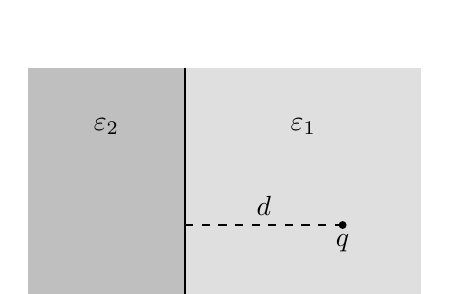
\begin{tikzpicture}
            \fill[gray!25](0, 0)rectangle(3, 3);
            \fill[gray!50](0, 0)rectangle(-2, 3);
            \node at(1.5, 2.25){$\varepsilon_1$};
            \node at(-1, 2.25){$\varepsilon_2$};
            \draw[thick](0, 0)--(0, 3);
            \draw[dashed](0, 1)--(2, 1)node[midway, above]{$d$};
            \fill[black](2, 1)circle(.05)node[below]{$q$};
        \end{tikzpicture}
    \end{center}
    为了计算$z>0$部分的电位,在$z<0$部分与$q$对称的位置放置镜像电荷$q'$:
    \[
        \Phi_1=\frac1{4\pi\varepsilon_1}\biggkh{\frac q{R_1}+\frac{q'}{R_2}},\quad z>0;
    \]
    为了计算$z<0$部分的电位,在$q$的位置替换为镜像电荷$q''$:
    \[
        \Phi_2=\frac1{4\pi\varepsilon_2}\frac{q''}{R_1},\quad z<0.
    \]
    由边界条件: 
    \begin{align*}
        \begin{cases}
            \varepsilon_1E_{1z}=\varepsilon_2E_{2z}\\
            E_{1\rho}=E_{2\rho}
        \end{cases}\Rightarrow\quad
        \begin{cases}
            q-q'=q''\\
            \frac{q+q'}{\varepsilon_1}=\frac{q''}{\varepsilon_2}
        \end{cases}\Rightarrow\quad
        \begin{cases}
            q'=-\frac{\varepsilon_2-\varepsilon_1}{\varepsilon_2+\varepsilon_1}q\\[1ex]
            q''=\frac{2\varepsilon_2}{\varepsilon_2+\varepsilon_1}q
        \end{cases}
    \end{align*}
    $\varepsilon_2>\varepsilon_1$时,$q,q'$符号相反,$\varepsilon_1$内的电场线外凸;
    
    $\varepsilon_2<\varepsilon_1$时,$q,q'$同号,$\varepsilon_1$内电场线内凸。
    \tcblower 
    由式(\ref{eqn:Pn2-Pn1}),$z=0$上极化电荷面密度为
    %\bm P_i=(\varepsilon_i-\varepsilon_0)\bm E_i=-(\varepsilon_i-\varepsilon_0)\nabla\Phi(0^\pm).
    \[
        \sigma_\text{pol}=P_{2z}-P_{1z}=-\frac q{2\pi}\frac{\varepsilon_0(\varepsilon_2-\varepsilon_1)}{\varepsilon_1(\varepsilon_2+\varepsilon_1)}\frac d{(\rho^2+d^2)^{3/2}}.
    \]
    当$\varepsilon_2\gg\varepsilon_1$时,介质$\varepsilon_2$表现很像导体($q'=-q$)。
\end{example}
\begin{example}{匀强电场中的介质球}{dielectric sphere in uniform electric field}
    半径为$a$的介质球$\varepsilon$在匀强电场$E_0$中。其电势
    \begin{alignat*}{2}
        \Phi_1&=\sum\fmto\ell 0A_\ell r^\ell P_\ell(\cos\theta),&\quad&r<a\\
        \Phi_2&=\sum\fmto\ell 0\bigfkh{B_\ell r^\ell+C_\ell r^{-(\ell+1)}}P_\ell(\cos\theta),&&r>a
    \end{alignat*}
    又$r\to\infty$时,$\Phi_2\simeq -E_0r\cos\theta$,故 
    \[
        \Phi_2=-E_0r\cos\theta+\sum\fmto\ell 0C_\ell r^{-(\ell+1)}P_\ell(\cos\theta),
    \]
    由边界条件……
    \[
        \Phi=\begin{cases}
            -\frac{3}{\varepsilon_\r+2}E_0r\cos\theta,&r<a\\
            -E_0r\cos\theta+\biggkh{\frac{\varepsilon_\r-1}{\varepsilon_\r+2}}E_0\frac{a^3}{r^2}\cos\theta,&r>a
        \end{cases}
    \]
    因此介质球内是匀强电场
    \[
        E_\text{in}=\frac{3}{\varepsilon_\r+2}E_0;
    \]
    介质球外相当于外加场$E_0$加上原点的电偶极场,偶极矩朝向电偶极场的方向
    \[
        \bm p=4\pi\varepsilon_0\biggkh{\frac{\varepsilon_\r-1}{\varepsilon_\r+2}}a^3\bm E_0,
    \]
    球体内的电极化强度
    \begin{equation}
        \label{eqn:P-E}
        \bm P=(\varepsilon-\varepsilon_0)\bm E_\text{in}=3\varepsilon_0\biggkh{\frac{\varepsilon_\r-1}{\varepsilon_\r+2}}\bm E_0,
    \end{equation}
    因此表面极化电荷面密度:
    \[
        \sigma_\text{pol}=\bm P\cdot\uvec r=3\varepsilon_0\biggkh{\frac{\varepsilon_\r-1}{\varepsilon_\r+2}}E_0\cos\theta.
    \]
\end{example}
\subsubsection{分子极化率和电极化率}
在本节中,我们将讨论分子极化率(molecular polarizability)和电极化率(electric susceptibility) $\chi_\elc$之间的关系。%我们仅从给它列个大纲开始。

在稀薄(rarefied)介质中,宏观场与作用在任何分子或分子群上的场几乎没有区别。但在致密(dense)介质中,相邻分子的极化会产生一个内部场$\bm E_\text{in}$,所以分子上的总电场是$\bm E+\bm E_\text{in}$,内部场$\bm E_\text{in}$可以写成两项之差:
\[
    \bm E_\text{in}=\bm E_\text{near}-\bm E_p,
\]
$\bm E_\text{near}$是给定分子附近分子的实际作用,$\bm E_p$是由极化$\bm P$描述的以平均连续介质近似处理的分子的贡献。
对于包含很多分子的半径为$R$的球, 
\[
    \bm p=\frac{4\pi}3R^3\bm P,\quad \bm E_p=\frac3{4\pi R^3}\int_{r<R}\bm E\d v=-\frac{\bm P}{3\varepsilon_0}.
\]
对于大多数材料,可有效近似$\bm E_\text{near}=\bm 0$,故$\bm E_\text{in}=\bm P/3\varepsilon_0$。

定义分子极化率$\gamma_\text{mol}$为分子平均偶极矩$\ave{\bm p_\text{mol}}$与$\varepsilon_0$乘上分子处电场的比值。
\[
    \bm P=N\ave{\bm p_\text{mol}}=N\varepsilon_0\gamma_\text{mol}(\bm E+\bm E_\text{in})=N\gamma_\text{mol}\biggkh{\varepsilon_0\bm E+\frac{\bm P}3}.
\]
再与$\bm P=\varepsilon_0\chi_\elc\bm E,\enspace\varepsilon_\r=1+\chi_\elc$,得到Clausius-Mossotti方程
\begin{equation}
    \gamma_\text{mol}=\frac3N\frac{\chi_\elc}{\chi_\elc+3}=\frac3N\frac{\varepsilon_\r-1}{\varepsilon_\r+2}.
\end{equation}
这种关系对气体等稀释物质最适用。对于液体和固体,上式仅近似有效,特别是当介电常数很大时。
\paragraph{分子极化率的模型}
由谐振子模型
\[
    m\omega_0^2\bm x=e\bm E,\thus\bm p_\text{mol}=e\bm x=\frac{e^2\bm E}{m\omega_0^2},\thus\gamma_\text{mol}=\frac{e^2}{m\omega_0^2\varepsilon_0}.
\]
$\omega_0$为分子的固有频率。

常温常压(normal temperature and pressure, NTP)下,气体$\chi_\elc<10^{-3}$,固体和液体$\chi_\elc\sim 1$。

一般的,考虑不同能量的分子的Boltzmann分布,
\[
    \gamma_\text{mol}\simeq\frac{e^2}{m\omega_0^2\varepsilon_0}+\frac{p_0^2}{3\varepsilon_0\kB T}.
\]
$p_0$为分子固有偶极矩的大小。
\subsubsection{电介质中的静电能}
一般情况下,我们对电介质不作假设。可由微小功$\vd W$推出电介质中的静电能为
\[
    W=\intt_0^D\bm E\cdot\vd\bm D\d v.
\]
若介质是线性的,则
\begin{equation}
    W=\frac12\int_V\bm E\cdot\bm D\d v=\frac12\int_V\rho(\bm x)\Phi(\bm x)\d v.
\end{equation}
上式仅当介质是线性时才在宏观上成立。
\paragraph{电介质在极化过程中储存的能量}过程分电荷不变和电势不变;
\subparagraph{电荷分布不变过程}
若电介质放入前后源电荷分布$\rho(\bm x)$不变
\begin{align*}
    \D W&=\frac12\int_V(\bm E\cdot\bm D-\bm E_0\cdot\bm D_0)\d v\\
    &=\frac12\int_V(\bm E\cdot\bm D_0-\bm E_0\cdot\bm D)\d v+\frac12\int_V(\bm E+\bm E_0)\cdot\cancel{(\bm D-\bm D_0)}\d v\\
    &=-\frac12(\varepsilon-\varepsilon_0)\int_V\bm E\cdot\bm E_0\d v=-\frac12\int_V\bm P\cdot\bm E_0\d v,
\end{align*}
因此电介质的能量密度为
\begin{equation}
    w=-\frac12\bm P\cdot\bm E_0,
\end{equation}
%假设电介质移动了一个微小的位移$\vd x$,系统的总能量发生变化$\vd W$,则电介质受到的外力
%F=-\biggkh{\frac{\vd W}{\vd x}}_Q,
\subparagraph{电势不变过程}下面分析在电势分布不变情形下,电介质放入前后的能量变化(不能用$\vd W_V=-F\vd x$计算)。
\[
    \vd W=\int_V\Phi(\bm x)\vd\rho(\bm x)\d v
\]
又对于线性介质,
\[
    \vd W=\frac12\int_V\bigfkh{\rho(\bm x)\vd\Phi(\bm x)+\Phi(\bm x)\vd\rho(\bm x)}\d v,
\]
故$\rho(\bm x)\vd\Phi(\bm x)=\Phi(\bm x)\vd\rho(\bm x)$。

在电势分布不变情形下,电介质放入的过程可以分为两步:
\begin{compactenum}
    \item 断开电极板和电源的接触,移动电介质,这一过程中电荷分布不变,
    \[
        \vd W_1=\frac12\int_V\bigfkh{\rho(\bm x)\vd\Phi_1(\bm x)+0}\d v;
    \]
    \item 将极板与电源相连,电势恢复到初始值,$\vd\Phi_1+\vd\Phi_2=0$
    \[
        \vd W_2=\frac12\int_V\bigfkh{\rho(\bm x)\vd\Phi_2(\bm x)+\Phi(\bm x)\vd\rho_2(\bm x)}\d v=-2\vd W_1.
    \]
\end{compactenum}
因此$\vd W=\vd W_1+\vd W_2=-\vd W_1$,从而
\[
    \vd W_V=-\vd W_Q.
\]
力
\[
    F=-\biggkh{\frac{\vd W}{\vd x}}_Q=\biggkh{\frac{\vd W}{\vd x}}_V.
\]
\clearpage
\section{静磁学、时变场}
\label{sec:magnetostatics}
本章主要介绍静磁学(magnetostatics)的内容,与前几章介绍的静电学在多处均有呼应。%当然,本文为节省篇幅省略了一些科学史的介绍及磁学的发展研究历程,感兴趣的读者可以自行查找相关资料了解。同时,对于一些过于基础性的概念也仅仅只做大致的描述。
类似于静电学,我们建立了静磁学的基本方程组,通过几个边值问题阐述了静磁学问题的处理方法。%(如均匀带电圆环在全空间产生的磁场……)。
%,……
%第三节介绍似稳场(quasi-static field)理论,……

第二节介绍Faraday定律,将静电学和静磁学中的恒稳态问题变为与时间有关的时变场(time-varying field)问题。

\subsection{磁感应强度、电流密度}
%值得注意的是,
磁场(magnetic field)的基本规律最早并不是直接根据人类对磁性材料的接触中得出的,原因在于静磁学和静电学存在一个根本上的差别:没有自由磁荷(free magnetic charge)的存在。在磁学中,基本单元是磁偶极子\footnote{就是高中物理里的小磁针模型。}(magnetic dipole)。磁场的磁感应强度\footnote{也称磁通密度(magnetic-flux density)}(magnetic induction) $\bm B$其方向被定义为处在该磁场中的磁偶极矩$\bm\mu$的方向,其大小可以由磁偶极矩$\bm\mu$所受力矩$\bm N$来衡量:
\begin{equation}
    \bm N=\bm\mu\times\bm B.
\end{equation}
另外通过Ørsted等人的实验,我们可以知道磁场是由电流(current)产生的。电流相当于运动电荷,用电流密度(current density)矢量$\bm J$描述:
\begin{equation}
    \bm J:=\rho\bm v,
\end{equation}
其大小为单位时间流过单位面积的电荷量,其方向为电荷运动的方向。
\paragraph{连续性方程}
由于电荷守恒(conservation of charge),空间中固定一点的电荷量不会有源项,因此
\begin{equation}
    \label{eqn:continuity}
    \pv\rho t+\div\bm J=0,
\end{equation}
上式称为连续性方程(continuity equation)。上式也可通过另一种方式推导:考虑空间一体积微元$V$,其内电荷量不随时间改变:
\[
    \dv{(\rho V)}t=\dv\rho tV+\rho\dv Vt=0,
\]
由于$\rho=\rho(x,y,z,t)$是时空的函数,其全微分为
\[
    \d\rho=\pv\rho t\d t+\pv\rho x\d x+\pv\rho y\d y+\pv\rho z\d z,
\]
两端除以$\d t$,得到其迁移导数(convective derivative)为
\[
    \dv\rho t=\pv\rho t+\pv\rho xv_x+\pv\rho yv_y+\pv\rho zv_z=\pv\rho t+\bm v\cdot\nabla\rho;
\]
而体积元的变化率
\[
    \dv Vt=\oint_{\p V}\bm v\cdot\d\bm a=\int_V\div\bm v\d V=V\div\bm v.
\]
因此 
\[
    \dv\rho t+\rho\div\bm v=\pv\rho t+\bm v\cdot\nabla\rho+\rho\div\bm v=\pv\rho t+\div(\rho\bm v)=0,
\]
上式即(\ref{eqn:continuity})。
\paragraph{稳恒电流}
稳恒(steady-state)磁现象满足空间各处的$\rho$不变,于是%对于静磁学,
\begin{equation}
    \div\bm J=0.
\end{equation}
%我们从电流与磁感应强度之间的关系出发,建立静磁学基本定律。
\subsection{Biot-Savart定律}
%尽管磁现象的发现有很悠久的历史,但直到建立了电流和磁场之间的联系,磁现象才得到定量描述。
为了描述电流在激发磁场时的作用,我们引入电流元(current element)的概念:$\d\bm\ell$是通电流$I$的导线的长度元,指向电流方向,则电流元为$I\d\bm\ell$。
\begin{theorem}{Biot-Savart定律}{Biot and Savart Law}
    原点处电流元$I\d\bm\ell$在$\bm x$处激发的磁感应强度元$\d\bm B$为
    \begin{equation}
        \label{eqn:B-S law}
        \d\bm B=k\frac{I\d\bm\ell\times\bm x}{|\bm x|^3},\quad k=\frac{\mu_0}{4\pi},
    \end{equation} 
    真空磁导率$\mu_0=\SI{4\pi e-7}{N/A^2}.$
\end{theorem}
尽管式(\ref{eqn:B-S law})与点电荷电场强度(\ref{eqn:E of q})有相似的形式,但%电流元$I\d\bm\ell$并不能视为点电荷$q$的磁场对应,
%只有把电流元看做对连续集合(电流回路)求和中的一个元素时才有意义,
式(\ref{eqn:B-S law})只有在积分中才有意义,
因为电流元本身并不满足连续性方程(\ref{eqn:continuity})。
\footnote{摆脱这个困难的一种办法是:将电流元$I\d\bm\ell$换成运动电荷$q\bm v$
\[
    \bm B=k\frac{q\bm v\times\bm x}{|\bm x|^3}.
\]
但这个表达式与时间相关,并且只有当电荷速度$v\ll c$且加速度可忽略不计时才成立。
而式(\ref{eqn:B-S law})是精确的原因在于:
对于一个电荷单元趋于0且电荷数目趋于无穷大的稳恒电流系统,精确的相对论电磁场理论(包括加速度效应)将给出一个静磁场,并且等于式(\ref{eqn:B-S law})遍历电流积分所得的场。所以我们采用(\ref{eqn:B-S law})。}
\begin{example}{无限长直导线的磁场}{B of straight line}
    $z$轴上的长直导线电流方向为$+z$,距离其$\rho$处的磁感应强度大小为
    \[
        B_\phi(\rho)=\frac{\mu_0}{4\pi}\int\iti\frac{I\rho\d z}{(z^2+\rho^2)^{3/2}}=\frac{\mu_0}{2\pi}\frac I\rho.
    \]
    方向服从右手定则,即$\uvec\phi$方向。
\end{example}
电流元件$I\d\bm\ell$在磁感应强度$\bm B$中所受的力
\[
    \d\bm F=I\d\bm\ell\times\bm B.
\]
换成电荷得到Lorentz力
\begin{equation}
    \bm F=q\bm v\times\bm B.
\end{equation}
\begin{example}{闭合回路之间的力}{F of 2 closed lines}
    由闭合电流回路2产生的闭合电流回路1的总力:
    \[
        \bm F_{12}=\frac{\mu_0}{4\pi}I_1I_2\oint\bs3\oint\frac{\d\bm\ell_1\times(\d\bm\ell_2\times\bm x_{12})}{|\bm x_{12}|^3};
    \]
    利用(\ref{eqn:bac-cab})化为更对称的形式:
    %\bm A\times(\bm B\times\bm C)=\bm B(\bm A\cdot\bm C)-\bm C(\bm A\cdot\bm B)
    \[
        \bm F_{12}=\frac{\mu_0}{4\pi}I_1I_2\biggfkh{\oint\bs3\cancel{\oint\frac{\bm x_{12}\cdot\d\bm\ell_1}{|\bm x_{12}|^3}}\d\bm\ell_2-\oint\bs3\oint\frac{\bm x_{12}}{|\bm x_{12}|^3}(\d\bm\ell_1\cdot\d\bm\ell_2)}.
    \]
    %第一项的环路积分为0,
    第二项是对称的,因此满足Newton第三定律。
\end{example}
\begin{example}{两条长平行直导线之间的力}{F of 2 parallel lines}
    由例 \ref{exm:B of straight line},两条长平行直导线之间的力为
    \begin{equation}
        \dv F\ell=\frac{\mu_0}{2\pi}\frac{I_1I_2}d.
    \end{equation}
\end{example}
电流元可以写成电流密度$\bm J$的形式
\[
    I\d\bm\ell=\d q\bm v=(\rho\d v)\bm v=\bm J\d v,
\]
因此磁场中电流受到的力可以写成:
\[
    \bm F=\int_V\d q(\bm v\times\bm B)=\int_V\rho(\bm v\times\bm B)\d v=\int_V\bm J\times\bm B\d v.
\]
总力矩:
\[
    \bm N=\bm x\times\bm F=\int_V\bm x\times(\bm J\times\bm B)\d v.
\]
\subsubsection{Ampère定律}
利用电流密度,Biot-Savart定律(\ref{eqn:B-S law})可以写成旋度的形式
\begin{align}
    \label{eqn:B(x)}
    \bm B(\bm x)&=\frac{\mu_0}{4\pi}\int_V\bm J(\bm x')\times\frac{\bm x-\bm x'}{|\bm x-\bm x'|^3}\d v'\\
    &=\frac{\mu_0}{4\pi}\curl\int_V\frac{\bm J(\bm x')}{|\bm x-\bm x'|}\d v'.
\end{align}
由(\ref{eqn:divcurl}),可得$\bm B$的第一个微分方程:
\begin{equation}
    \label{eqn:divB}
    \div\bm B=0,
\end{equation}

现在我们希望知道$\bm B$的散度,利用(\ref{eqn:curlcurl})
\begin{align*}
    &\curl\biggfkh{\curl\frac{\bm J(\bm x')}{|\bm x-\bm x'|}}=\nabla\biggfkh{\div\frac{\bm J(\bm x')}{|\bm x-\bm x'|}}-\lapla\frac{\bm J(\bm x')}{|\bm x-\bm x'|}\\
    &\qquad=\nabla\biggfkh{\frac{\cancel{\div\bm J(\bm x')}}{|\bm x-\bm x'|}+\bm J(\bm x')\cdot\nabla\frac1{|\bm x-\bm x'|}}-\bm J(\bm x')\lapla\frac1{|\bm x-\bm x'|}.
\end{align*}
则
\[
    \curl\bm B=\frac{\mu_0}{4\pi}\biggfkh{-\nabla\int_V\bm J(\bm x')\cdot\nabla'\frac1{|\bm x-\bm x'|}\d v'+4\pi\bm J(\bm x)}
\]
对积分项进行分部积分:
\[
    \int_V\bm J(\bm x')\cdot\nabla'\frac1{|\bm x-\bm x'|}\d v'=\oint_{\p V}\frac{\cancel{\bm J(\bm x')\cdot\uvec n'}}{|\bm x-\bm x'|}\d a'-\int_V\frac{\cancel{\nabla'\cdot\bm J(\bm x')}}{|\bm x-\bm x'|}\d v'=0,
\]
\iffalse
\begin{align*}
    \curl\bm B&=\frac{\mu_0}{4\pi}\curl\biggfkh{\curl\int_V\frac{\bm J(\bm x')}{|\bm x-\bm x'|}\d v'}\\
    &\qquad\textcolor{gray}{\curl(\curl\bm A)=\nabla(\div\bm A)-\lapla\bm A}\\
    &=\frac{\mu_0}{4\pi}\biggfkh{\nabla\int_V\div\frac{\bm J(\bm x')}{|\bm x-\bm x'|}\d v'-\int_V\lapla\frac{\bm J(\bm x')}{|\bm x-\bm x'|}\d v'}\\
    &\qquad\textcolor{gray}{\div(\varphi\bm A)=A\cdot\nabla\varphi+\varphi\div\bm A}\\
    &=\frac{\mu_0}{4\pi}\biggfkh{\nabla\int_V\biggkh{\bm J(\bm x')\cdot\nabla\frac1{|\bm x-\bm x'|}+0}\d v'-\int_V\bm J(\bm x')\lapla\frac1{|\bm x-\bm x'|}\d v'}\\
    %=\frac{\mu_0}{4\pi}\biggfkh{-\nabla\int_V\bm J(\bm x')\cdot\nabla'\frac1{|\bm x-\bm x'|}\d v'+4\pi\bm J(\bm x)}\\
    &\qquad\textcolor{gray}{\int_V\bm A\cdot\nabla f\d v=-\int_Vf\div\bm A\d v+\oint_{\p V}f\bm A\cdot\uvec n\d a}\\
    &=\mu_0\bm J(\bm x)+\frac{\mu_0}{4\pi}\nabla\biggfkh{\int_V\frac{\cancel{\nabla'\cdot\bm J(\bm x')}}{|\bm x-\bm x'|}\d v'-\cancel{\oint_{\p V}\frac{\bm J(\bm x')\cdot\uvec n'}{|\bm x-\bm x'|}\cdot\d a'}};
\end{align*}
\fi
由此得到第二个微分方程:
\begin{equation}
    \label{eqn:curlB}
    \curl\bm B=\mu_0\bm J.
\end{equation}
两边取$S$的面积分
\[
    \int_S\curl\bm B\cdot\uvec n\d a=\mu_0\int_S\bm J\cdot\uvec n\d a.
\]
右边积分项即穿过$S$的电流$I$,可得Ampère定律:
\begin{theorem}{Ampère定律}{Ampere's law}
    \begin{equation}
        \label{eqn:Ampere}
        \oint_{\p S}\bm B\cdot\d\bm\ell=\mu_0I.
    \end{equation}
\end{theorem}
在高度对称的条件下,可利用Ampère定律得到磁感应强度的大小。
\subsection{矢量势}
\label{ssec:vector potential}
由于$\bm B$可以写成旋度的形式,可
定义矢量势(vector potential)满足
\begin{equation}
    \bm B=\curl\bm A.
\end{equation}
但满足上式的$\bm A$并不唯一。对$\bm A$进行规范(gauge)变换:
\[
    \bm A'=\bm A+\nabla\varLambda,
\]
上式对于任意的$\varLambda$仍成立:
\[
    \curl\bm A'=\curl(\bm A+\nabla\varLambda)=\curl\bm A+\bm 0=\bm B.
\]
因此有必要选定一个额外的限制条件,一个方便的选择是Coulomb规范:
\begin{equation}
    \div\bm A=0.
\end{equation}
从而$\lapla\varLambda=0$,在无边界条件时,$\varLambda=\cns$,$\bm A$形式即最简洁的:
\begin{equation}
    \label{eqn:A-J}
    \bm A(\bm x):=\frac{\mu_0}{4\pi}\int\frac{\bm J(\bm x')}{|\bm x-\bm x'|}\d v',
\end{equation}

我们也可以得到$\bm A$三个分量的Laplace方程:
\[
    \curl\bm B=\curl(\curl\bm A)=\nabla(\cancel{\div\bm A})-\lapla\bm A.
\]
即
\begin{equation}
    \lapla\bm A=-\mu_0\bm J.
\end{equation}
\clearpage
\subsection{磁矩}
\begin{example}{环形电流回路的磁场}{B of loop current}
    在球坐标中,电流密度$\bm J$仅有$\phi$分量
    \[
        J_\phi=I\sin\theta'\vd(\cos\theta')\frac{\delta(r'-a)}a.
    \]
    故矢量势$\bm A$也仅有$\phi$分量:
    \begin{align*}
        A_\phi&=\frac{\mu_0}{4\pi}\int\frac{J_\phi}{|\bm x-\bm x'|}\d v'\\
        &=\frac{\mu_0I}{4\pi a}\int\zti\bs5\oint\frac{\sin\theta'\vd(\cos\theta')\vd(r'-a)r^2\d\Omega'\d r'}{\sqrt{r^2+r'^2-2rr'(\cos\theta\cos\theta'+\sin\theta\sin\theta'\cos\phi')}}\\
        &=\frac{\mu_0Ia}{4\pi}\int_0^{2\pi}\frac{\cos\phi'\d\phi'}{\sqrt{a^2+r^2-2ar\sin\theta\cos\phi'}}\\
        &=\frac{\mu_0I}\pi\frac{a}{\sqrt{a^2+r^2+2ar\sin\theta}}\biggfkh{\biggkh{\frac2{k^2}-1}K(k)-\frac2{k^2}E(k)}.%\frac{(2-k^2)K(k)-2E(k)}{k^2}.
    \end{align*}
    其中 
    \[
        k^2:=\frac{4ar\sin\theta}{a^2+r^2+2ar\sin\theta}.
    \]
    $K(k),E(k)$为第一、二类完全椭圆积分
    \begin{alignat*}{2}
        K(k)&=\int_0^1\frac{\d x}{\sqrt{(1-x^2)(1-k^2x^2)}}&,\enspace|k|&<1\\
        E(k)&=\int_0^1\sqrt{\frac{1-k^2x^2}{1-x^2}}\d x&|k|&<1.
    \end{alignat*}
    \begin{center}
        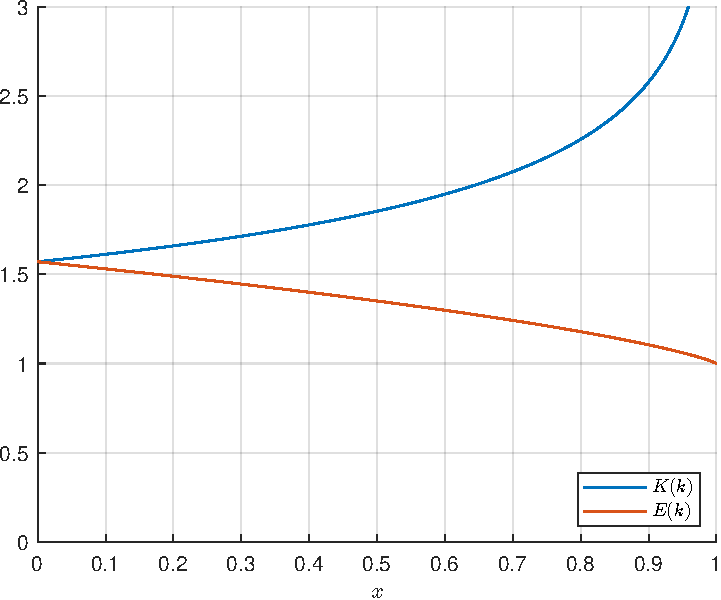
\includegraphics[width=7cm]{graphs/ellipseKE.pdf}
        \tikzchap 第一、二类完全椭圆积分
    \end{center}
    当$r\gg a$或$r\ll a$或$\theta\to 0$时,
    \[
        A_\phi(r,\theta)=\frac{\mu_0I}4\frac{a^2r\sin\theta}{(a^2+r^2)^{3/2}}\biggfkh{1+\frac{15}8\biggkh{\frac{ar\sin\theta}{a^2+r^2}}^2+\cdots},
    \]
    因此对于$r\gg a$处的远场
    \begin{align*}
        B_r&=\frac1{r\sin\theta}\pp\theta(\sin\theta A_\phi)=\frac{\mu_0Ia^2}2\frac{\cos\theta}{r^3},\\
        B_\theta&=-\frac1r\pp r(rA_\theta)=\frac{\mu_0Ia^2}4\frac{\sin\theta}{r^3},
    \end{align*}
    与电偶极矩的电场(\ref{eqn:edipole-E})比较,可定义环形电流的磁偶极矩(magnetic dipole moment)大小
    \[
        m=I\cdot\pi a^2,
    \]
    沿$+z$方向,从而 
    \begin{align}
        \bm A&=\frac{\mu_0m\sin\theta}{4\pi r^2}\uvec\phi;\\
        \bm B&=\frac{\mu_0m}{4\pi r^3}(2\cos\theta\uvec r+\sin\theta\uvec\theta).
    \end{align}
\end{example}
我们现在考虑一般的电流分布在一个小(相对于感兴趣区域的尺度)的空间区域中的性质。
\footnote{这个问题可以用矢量球谐函数来做一个完整的处理,类似于静电多极展开。这些将在第9章多极辐射中介绍,我们在这里只满足于最低的近似阶。}
若$x\gg x'$,矢量势的分量可以被展开为:
\begin{equation}
    \label{eqn:A approx}
    A_\alpha(\bm x)=\frac{\mu_0}{4\pi}\biggfkh{\frac1{|\bm x|}\cancel{\int_V J_\alpha(\bm x')\d v'}+\frac{\bm x}{|\bm x|^3}\cdot\int_V J_\alpha(\bm x')\bm x'\d v+\cdots}
    \tag{$\ast$}
\end{equation}
下面我们用一些数学上的小tricks:
\[
    \oint_{\p V}fg\bm J\cdot\uvec n'\d a'=\int_V(g\bm J\cdot\nabla'f+f\bm J\cdot\nabla'g+fg\cancel{\nabla'\cdot\bm J})\d v'=0.
\]
将$f,g$赋予特定的形式,可以得到
\begin{alignat*}{2}
    \int_V J_\alpha \d v'&=0,&\qquad (f=1,\enspace g=x_\alpha');\\
    \int_V(x_\alpha'J_\beta+x_\beta'J_\alpha)\d v'&=0,&(f=x_\alpha',\enspace g=x_\beta')\\
    \int_V x_\alpha'J_\alpha\d v'&=0,&(f=g=x_\alpha').
\end{alignat*} 
\begin{definition}{全反对称张量}{Levi-Civita symbol}
    引入全反对称张量(Levi-Civita symbol)
    \begin{equation}
        \epsilon_{\alpha\beta\gamma}=\begin{cases}
            1,&(\alpha\beta\gamma)=(123)\\
            -1,&(\alpha\beta\gamma)=(321)\\
            0,&\text{otherwise}
        \end{cases}
    \end{equation}
    一般的定义:$\epsilon_{1\cdots n}=1$,置换任意两个下标则反号,下标相同则为0。
\end{definition}
利用全反对称张量,我们可以将叉乘的结果记作
\begin{equation}
    (\bm a\times\bm b)_\alpha=\sum_{\beta,\gamma}\epsilon_{\alpha\beta\gamma}a_\beta b_\gamma.
\end{equation}
由此可得(\ref{eqn:A approx})中的积分项
\[
    \bm x'\cdot\int_V\bm x'J_\alpha\d v'=-\frac12\biggfkh{\bm x\times\int_V(\bm x'\times\bm J)\d v'}_\alpha.
\]
可定义磁矩密度(magnetic moment density)或磁化强度(magnetization)
\begin{equation}
    \bm M:=\frac12\bm x\times\bm J.
\end{equation}
其体积分为磁偶极矩(magnetic dipole moment)简称磁矩
\begin{equation}
    \bm m=\frac12\int_V\bm x'\times\bm J(\bm x')\d v'.
\end{equation}
因此式(\ref{eqn:A approx})中,矢量势的最低阶非零项
\begin{equation}
    \bm A(\bm x)=\frac{\mu_0}{4\pi}\frac{\bm m\times\bm x}{|\bm x|^3}.
\end{equation}
进而磁感应强度与电偶极矩电场(\ref{eqn:edipole-E with delta})形式相似:
\begin{equation}
    \bm B(\bm x)=\frac{\mu_0}{4\pi}\biggfkh{\frac{3\uvec n(\bm m\cdot\uvec n)-\bm m}{|\bm x|^3}+\frac{8\pi}3\bm m\vd(\bm x)}.
\end{equation}
因此,远离任何局域电流分布的磁场就是一个磁偶极子的磁场。
\begin{example}{电流回路的磁矩}{m of I}
    平面$S$上的电流回路的磁矩
    \begin{align*}
        \bm m=\frac12\oint_{\p S}\bm x\times I\d\bm\ell=IS\uvec n.
    \end{align*}
    与例 \ref{exm:B of loop current} 中的定义一致。
\end{example}
\begin{example}{带电粒子轨道角动量的磁矩}{m of L}
    带电粒子的磁矩与其轨道角动量$\bm L=m\bm x\times\bm v$有关:
    \[
        \bm m=\frac12q\bm x\times\bm v=\frac q{2m}\bm L.
    \]
\end{example}
局部电流分布的磁场体积分
\[
    \int_{r<R}\bm B(\bm x)\d v=\begin{cases}
        \frac{2\mu_0}3\bm m,&\text{球内电流}\\[1ex]
        \frac{4\pi}3R^3\bm B(\bm 0),&\text{球外电流}
    \end{cases}.
\]
\subsubsection{磁矩的力、力矩和能量}
外部磁感应强度$\bm B(\bm x)$中电流密度$\bm J(\bm x)$受到的总力
\[
    \bm F=\int_V\bm J(\bm x)\times\bm B(\bm x)\d v\simeq(\bm m\times\nabla)\times\bm B.
\]
化简为
\[
    \bm F=\nabla(\bm m\cdot\bm B)-\bm m\cancel{(\div\bm B)}.
\]
力矩与作用在磁偶极子上的力矩表达式相同:
\[
    \bm N=\int_V\bm x'\times(\bm J\times\bm B)\d v'\simeq\bm m\times\bm B(\bm 0),
\]
上式也可作为定义磁感应强度的一种方法。

由$\bm F=-\nabla U$,可定义磁矩的势能为
\[
    U=-\bm m\times\bm B,
\]
$U$并不是外磁场中磁矩的总能量,因为它不包含产生$\bm m$并维持$\bm m$恒定所需的能量。另外,当$\bm m$和$\bm B$方向相同时,$U$最低,因此磁矩倾向于偏转自己平行于磁场。
\subsection{宏观介质静磁学}
在物质中,由原子电子贡献的有效(effective)原子电流和本征(intrinsic)磁矩产生的偶极场在原子尺度上变化非常明显。因此在宏观观测时,我们也需要对微观取空间平均\footnote{不需要对时间平均。}:
\begin{equation}
    \label{eqn:divB-macro}
    \div\bm B_\text{micro}=0,\thus\div\bm B=0.
\end{equation}
在$\bm x'$由一个小体积的$\D V$产生的矢量势
\[
    \D\bm A(\bm x)\simeq\frac{\mu_0}{4\pi}\biggfkh{\frac{\bm J(\bm x)'}{|\bm x-\bm x'|}+\frac{\bm M(\bm x')\times(\bm x-\bm x')}{|\bm x-\bm x'|^3}}\D V.
\]
其中宏观磁矩密度
\[
    \bm M(\bm x):=\sum_iN_i\ave{\bm m_i},
\]
积分之
\[
    \bm A(\bm x)=\frac{\mu_0}{4\pi}\int_V\frac{\bm J(\bm x')+\nabla'\times\bm M(\bm x')}{|\bm x-\bm x'|}\d v'
\]
因此 
\[
    \curl\bm B=\mu_0(\bm J+\curl\bm M),
\]
其中$\bm J_\text M:=\curl\bm M$是有效电流密度。
定义磁场强度(magnetic field)
\begin{equation}
    \bm H:=\frac{\bm B}{\mu_0}-\bm M.
\end{equation}
从而 
\begin{equation}
    \label{eqn:curlH}
    \curl\bm H=\bm J.
\end{equation}
式(\ref{eqn:divB-macro})和(\ref{eqn:curlH})考虑了有效原子电流的贡献,是(\ref{eqn:divB})和(\ref{eqn:curlB})的宏观对应。
\paragraph{本构关系}
下面我们介绍$\bm H$和$\bm B$的本构关系。对于各向同性抗磁性(diamagnetic)和顺磁性(paramagnetic)物质,有简单的线性关系:
\[
    \bm B=\mu\bm H,
\]
$\mu$为磁导率(permeability)。对于顺磁性物质,$\mu\gtrapprox\mu_0$;抗磁性物质$\mu\lessapprox\mu_0$。铁磁性(ferromagnetic)物质的$\mu$与$\bm H$的关系较为复杂,存在磁滞现象(hysteresis),但由于其$\mu\gg\mu_0$,有时可对边界条件作出简化假设。
\paragraph{表面分布}
考虑介质界面上$\bm B$和$\bm H$的分布,我们可以得到:
\begin{align}
    \label{eqn:Bn2-Bn1}
    (\bm B_2-\bm B_1)\cdot\uvec n_{21}&=0,\\
    \label{eqn:Ht2-Ht1}
    (\bm H_2-\bm H_1)\times\uvec n_{21}&=\bm J_\text S,
\end{align}
当$\mu_1\gg\mu_2$时,$H_{2\text n}\gg H_{1\text n}$,磁场$\bm H_2$与边界面垂直。所以,极高磁导率材料表面上$\bm H$的边界条件与导体表面上$\bm E$的边界条件相同:
\begin{center}
	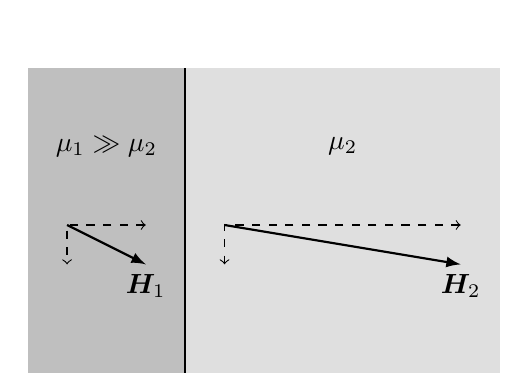
\begin{tikzpicture}
		\fill[gray!25](0, 0)rectangle(4, 4);
		\fill[gray!50](0, 0)rectangle(-2, 4);
		\node at(-1, 3){$\mu_1\gg\mu_2$};
		\node at(2, 3){$\mu_2$};
		\draw[thick](0, 0)--(0, 4);
		\draw[dashed, <->](-.5, 2)--(-1.5, 2)--(-1.5, 1.5);
		\draw[thick, -latex](-1.5, 2)--(-.5, 1.5)node[below]{$\bm H_1$};
		\draw[dashed, <->](3.5, 2)--(.5, 2)--(.5, 1.5);
		\draw[thick, -latex](.5, 2)--(3.5, 1.5)node[below]{$\bm H_2$};
	\end{tikzpicture}
	\tikzchap 极高磁导率材料表面的$\bm H$表现
\end{center}
因此,我们可以把静电势理论用于磁场上,高磁导率材料的表面是近似的等势面。这种类比在许多磁铁设计问题中用到:先决定场的形式,然后把极面设计成等势面的形状。
\begin{example}{}{}
    对于真空中的极高磁导率材料,若其表面无电流,则
    \[
        H_\parallel=H_{0,\parallel},\quad B_\perp=B_{0,\perp},
    \]
    因此材料内磁场
    \[
        B^2=B_{0,\perp}^2+\frac{\mu^2}{\mu_0^2}B_{0,\parallel}^2.
    \]
    两边同除$\mu$便得到了能量密度的形式,由于材料中储存的能量是有限的,故$B_{0,\parallel}=0$
\end{example}
\subsubsection{静磁学中的边界条件问题}
%对于磁化材料外部的磁场问题,
若材料是磁导率$\mu\gg\mu_0$的硬铁磁体(其磁矩密度$\bm M$与外场无关),则材料外表面上的$\bm B$垂直于界面,内表面上的$\bm B$平行于界面。如果其内没有电流($\bm J=\bm0$),则可引入磁势$\Phi_\text M$并解其Laplace方程。
\begin{equation}
    \bm H=-\nabla\bm\Phi_\text M,\quad\lapla\Phi_\text M=-\rho_\text M=\div\bm M.
\end{equation}
若无边界条件,则有解
\[
    \Phi_\text M=-\frac1{4\pi}\int_V\frac{\nabla'\cdot\bm M(\bm x')}{|\bm x-\bm x'|}\d v',
\]
若$\bm M$是局域的,则在$x\gg x'$的地方
\[
    \Phi_\text M\simeq\frac{\bm m\cdot\bm x}{4\pi r^3},\quad\bm m=\int_V\bm M\d v.
\]
但是我们仍需面对有边界条件的情形,在边界$\p V$处$\bm M$瞬间变为0,运用静电学中的结论:
\begin{equation}
    \label{eqn:PhiM with boundary}
    \Phi_\text M=-\frac1{4\pi}\int_V\frac{\nabla'\cdot\bm M(\bm x')}{|\bm x-\bm x'|}\d v'+\frac1{4\pi}\oint_{\p V}\frac{\bm M(\bm x')\cdot\uvec n'}{|\bm x-\bm x'|}\d a',
\end{equation}
若铁磁体是均匀磁化的,则$\div\bm M=0$,第一项为0。

我们接着求矢量势,由于$\bm J=\bm 0$,仅剩有效电流密度项
\begin{equation}
    \lapla\bm A=-\mu_0(\bm 0+\curl\bm M),
\end{equation}
可得
\begin{equation}
    \label{eqn:A with boundary}
    \bm A=\frac1{4\pi}\int_V\frac{\nabla'\times\bm M(\bm x')}{|\bm x-\bm x'|}\d v'+\frac1{4\pi}\oint_{\p V}\frac{\bm M(\bm x')\times\uvec n'}{|\bm x-\bm x'|}\d a',
\end{equation}
上式两项分别代表有效电流密度$\bm J_\text M$和有效面电流密度$\bm J_\text S$的贡献
\begin{align}
    \bm J_\text M&=\curl\bm M;\\
    \bm J_\text S&=\bm M\times\uvec n.
\end{align}
\begin{example}{均匀磁化球}{uniform magnetized sphere}
    真空中半径为$a$的球,其具有均匀的永久磁化强度$\bm M=M_0\uvec z$。应用式(\ref{eqn:PhiM with boundary})
    \[
        \Phi_\text M(r,\theta)=0+\frac1{4\pi}\oint_{r'=a}\frac{M_0\cos\theta'}{|\bm x-\bm x'|}\cdot a^2\d\Omega',
    \]
    进行球谐函数展开,式(\ref{eqn:1/|x-x'|=YY})仅有$\ell=1,\enspace m=0$项保留,且
    \[
        \cos\theta'=\sqrt{\frac{4\pi}3}Y_{10}(\theta',\phi'),
    \]
    故
    \[
        \Phi_\text M(r,\theta)=\frac13M_0a^2\cdot\frac{r_<}{r_>}\cos\theta.
    \]
    %$r_<,r_>$是$r,a$中的较小/大者。

    球内,$r_<=r,\enspace r_>=a$,表现为匀强磁场:
    \[
        \Phi_\text M=\frac13M_0r\cos\theta,\quad \bm H_\text{in}=-\frac13\bm M,\enspace\bm B_\text{in}=\frac{2\mu_0}3\bm M;
    \]
    球外,$r_<=a,\enspace r_>=r$,表现为磁偶极子(没有更高阶的项):
    \[
        \Phi_\text M=\frac{M_0a^3}3\frac{\cos\theta}{r^2}=\frac{\bm m\cdot\bm x}{4\pi r^3},\quad\bm m=\frac{4\pi}3a^3\bm M.
    \]
    $\bm B$线是连续的闭合曲线,而$\bm H$线不是。
    \tcblower
    也可通过矢量势的方法:
    \[
        A_\phi(r,\theta)=\frac{\mu_0}3M_0a^2\cdot\frac{r_<}{r_>^2}\sin\theta.
    \]
\end{example}
\begin{example}{外场下的磁化球}{magnetized sphere in external field}
    续例 \ref{exm:uniform magnetized sphere},在全空间叠加一匀强场$\bm B_0=\mu_0\bm H_0$,便成为外场下的磁化球问题,球内场强为
    \[
        \bm H_\text{in}=\bm B_0+\frac{2\mu_0}3\bm M,\quad\bm H_\text{in}=\bm H_0-\frac13\bm M,
    \]
    如果球是顺磁或抗磁的,那么$\bm M$便是由外场引起的,且$\bm B_\text{in}=\mu\bm H_\text{in}$,从而得到与电介质(\ref{eqn:P-E})很相似的结果:
    \begin{equation}
        \label{eqn:M-B}
        \bm M=\frac3{\mu_0}\biggkh{\frac{\mu_\r-1}{\mu_\r+2}}\bm B_0.
    \end{equation}
    如果球是铁磁的,那么便可以得到$\bm B_\text{in}$和$\bm H_\text{in}$的限制关系:
    \[
        \bm B_\text{in}+2\mu_0\bm H_\text{in}=3\bm B_0,
    \]
    上式可以在磁滞图上画一条直线,并会产生交点。
\end{example}
\begin{example}{外场下的磁化球壳}{magnetized sphere shell in external field}
    内外半径为$a,b$的球壳磁导率为$\mu$,放置在匀强磁场$\bm B_0$中,由于没有电流可应用磁势求解
    \[
        \lapla\Phi_\text M=0
    \]
    由式(\ref{eqn:Phi(r, theta)}),再加上$r\to\infty$时$\bm H=\bm H_0$的条件,可写出磁势的形式解,再通过边界条件
    \[
        \cdots
    \]
    \iffalse
    \begin{align*}
        \begin{cases}
            \edg{\pv{\Phi_\text{M,I}}\theta}_{r=a}=\edg{\pv{\Phi_\text{M,II}}\theta}_{r=a}\\[2ex]
            \edg{\pv{\Phi_\text{M,II}}\theta}_{r=b}=\edg{\pv{\Phi_\text{M,III}}\theta}_{r=b}
        \end{cases}
        \begin{cases}
            \mu_0\edg{\pv{\Phi_\text{M,I}}r}_{r=a}=\mu\edg{\pv{\Phi_\text{M,II}}r}_{r=a}\\[2ex]
            \mu_0\edg{\pv{\Phi_\text{M,II}}r}_{r=b}=\mu\edg{\pv{\Phi_\text{M,III}}r}_{r=b}
        \end{cases}
    \end{align*}
    \fi
    可得系数仅剩$\ell=1$项,壳内是一个匀强场:
    \[
        \Phi_\text M(r,\theta)=
        \begin{cases}
            a_1r\cos\theta,&r<a\\
            \ldots,&a<r<b\\
            -H_0r\cos\theta+\frac{d_1}{r^2}\cos\theta,&r>b
        \end{cases}
    \]
    当$\mu\gg\mu_0$时,壳内场强趋于0,这便是磁屏蔽效应。
\end{example}
最后探究了在一侧具有渐近均匀切向磁场的完全导电平面上的圆孔的影响,略。
\subsection{Faraday电磁感应定律}
\label{ssec:Faraday}
我们在前几章里论述了静电学和静磁学中的稳恒态问题。我们虽然用了相似的数学方法,但把电现象和磁现象当作相互独立的现象来处理。两者之间唯一的联系在于如下事实:\textit{磁场是由电流产生的,而电流就是运动的电荷。}
但当我们考虑与时间有关的问题时,电现象和磁现象的几乎独立的性质便会消失:随时间变化的磁场会产生电场,反之亦然。%这时我们必须说电磁场,而不能说电场或磁场.只有在狭

Faraday在探究时变磁场中电流表现的实验表面:
\begin{compactenum}
    \item 接通/断开临近电路的稳恒电流;
    \item 临近电路的稳恒电流相对于本电路移动;
    \item 将一根永磁体插入/抽出电路
\end{compactenum}
都会在电路中产生瞬态(transient)电流。Faraday把瞬态电流的产生解释为电路环绕磁通量(magnetic flux)%\footnote{本笔记中,$\Phi$已经被标量势占用了,$\phi$被方位角占用了,$\psi$和$\varphi$似乎还没人占用。}
\begin{equation}
    \varPhi:=\int_S\bm B\cdot\uvec n\d a
\end{equation}
的变化所引起的。变化的磁通量会再电路周围感感生(induce)一个电场驱动电路电荷运动形成电流,其电动势(electromotive force, emf)为
\begin{equation}
    \emf:=\oint_{\p S}\bm E'\cdot\d\bm \ell.
\end{equation}
$\bm E'$是在运动坐标系或介质中的电场。则Faraday的观测结果可总结为:
\begin{equation}
    \label{eqn:emf propto varPhi'}
    \emf\propto-\dv\varPhi t.
    \tag{$\ast$}
\end{equation}
其符号由Lenz定律决定:感生电流磁通量总是对抗磁通量的变化。
\paragraph{Galilean变换}
下面我们希望得到式(\ref{eqn:emf propto varPhi'})中的比例系数$k$,%事实上此系数已经可以从已有的单位制推出,而不像$\varepsilon_0$等需要引入新的单位。
我们将从已有单位制推导(而非定义)该比例系数。

在狭义相对论(special relativity)发现之前(或处理低速情况时),所有物理学家都公认(虽然不经常明确说出)物理定律在Galilean变换(transformation):
\begin{align*}
    \bm x'&=\bm x+\bm vt,\\
    t'&=t.
\end{align*}
下应该是不变的。$\bm v$是两个参考系之间的相对速度。也就是说,两个以恒定速度$\bm v$作相对运动的观察者看到的物理现象是一样的。%,只要这两组空间坐标和时间坐标的关系遵从Galilean变换:

Faraday从实验上证实电磁感应现象在Galilean变换下不变:无论是载电流的初级电路静止、次级电路运动;或者是次级电路静止、而载电流的初级电路作同样的相对运动,在次级电路中感生的电流是相同的。

现在讨论一个运动电路的法拉第定律,如果电路以恒定速度$\bm v$移动,则磁场的迁移导数为
\begin{align*}
    \dv{\bm B}t&=\pv{\bm B}t+(\bm v\cdot\nabla)\bm B\\
    &=\pv{\bm B}t+\curl(\bm B\times\bm v)+\cancel{(\bm B\cdot\nabla)\bm v}-\bm B(\cancel{\div\bm v})+\bm v(\cancel{\div\bm B}),
\end{align*}
即,
\begin{align*}
    \dd t\int_S\bm B\cdot\uvec n\d a=\int_S\pv{\bm B}t\cdot\uvec n\d a+\oint_{\p S}(\bm B\times\bm v)\cdot\d\bm\ell,
\end{align*}
因此 
\[
    \oint_{\p V}\bigkh{\bm E'-k\bm v\times\bm B}\d\bm\ell=-k\int_S\pv{\bm B}t\cdot\uvec n\d a.
\]
由Galilean变换下电场力和Lorentz力的形式,应有:
\[
    \bm E'=\bm E+\bm v\times\bm B,
\]
即$k=1$,因此Faraday定律可以写成等式:
\begin{equation}
    \label{eqn:Faraday}
    \emf=-\dv\varPhi t,
\end{equation}
并可由Stokes公式转化为微分形式
\begin{equation}
    \label{eqn:curlE-B}
    \curl\bm E=-\pv{\bm B}t.
\end{equation}
而%我们知道
静电场的旋度(\ref{eqn:curlE})为0!时变场将电场和磁场联系了起来。
\subsection{磁场的能量}
我们在前面讨论静磁场时,避开了场能和能量密度的问题。
因为
要建立电流的稳恒组态及有关的磁场,必定经过一段初始的瞬变期,在这期间,电流和磁场从零增到终值。存在这种随时间变化的场,就存在使电流源做功的感生电动势。因为按照定义,场的能量等于建立这场时所做的总功,所以我们必须考虑这些贡献。

保持电流恒定不变,
\[
    \vd W=\int_V\vd\bm A\cdot\bm J\d v=\int_V\bm H\cdot\vd\bm B\d v.
\]
对于顺磁性和抗磁性物质,$2\bm H\cdot\vd\bm B=\vd(\bm H\cdot\bm B)$
\[
    W=\frac12\int_V\bm A\cdot\bm J\d v=\frac12\int_V\bm H\cdot\bm B\d v.
\]

将一个磁导率为$\mu$的物体放进电流源固定不动的磁场$\bm B$中,前后能量发生变化
\[
    \D W=\frac12\int_V\bm M\cdot\bm B_0\d v.
\]
\subsubsectionstar{自感和互感}
对于$N$个不导磁的载流电路系统,总能量可以描述为:
\[
    W=\frac12\sum_{i=1}^NL_iI_i^2+\frac12\sum_{i=1}^N\sum_{j=1}^NM_{ij}I_iI_j.
\]
$L_i$是线圈$i$的自感(self-inductance),$M_{ij}$是线圈$i,j$之间的互感(mutual inductance),可以证明 
\[
    M_{ij}=M_{ji}.
\]

自感和互感可由
\[
    W=\frac12\int_V\bm J\cdot\bm A\d v.
\]
求出,用磁通量的形式即
\[
    L_i=\frac{\varPhi_{ii}}{I_i},\quad M_{ij}=\frac{\varPhi_{ij}}{I_j}.
\]
若电路是导磁的,则$W$的表达式不适用了,需要换为
\[
    W=\frac12\int_V\bm H\cdot\bm B\d v.
\]
后面还讨论了圆导线的自电感。
\subsectionstar{似稳场}
似稳场(quasi-static field)、涡流(eddy current)、磁扩散(magnetic diffusion)
\clearpage
\section{Maxwell方程组}
\label{sec:Maxwell}
\subsection{Maxwell位移电流}
在前面的讨论中,我们已经得到了关于电场和磁场的基本定律,分别是:
\begin{align*}
    \text{电场Gauss定律}&\,(\ref{eqn:divD})&\div\bm D&=\rho,\\
    \text{磁场Gauss定律}&\,(\ref{eqn:divB-macro})&\div\bm B&=0,\\
    \text{Ampère定律}&\,(\ref{eqn:curlH})&\curl\bm H&=\bm J,\\
    \text{Faraday电磁感应定律}&\,(\ref{eqn:curlE-B})&\curl\bm E&=-\pv{\bm B}t.
\end{align*}
%除了Faraday定律外,所有定律都是在稳恒态条件下得到的。
但在第 \ref{sec:magnetostatics} 章推导Ampère定律时,我们设定了稳恒电流条件$\div\bm J=0$,这在非稳恒态问题中便显然不适用了,而应该修正为连续性方程(\ref{eqn:continuity}):%与连续性方程不一致了。
%Maxwell受Faraday观察结果的启发,发现了方程组中的矛盾。
\[
    \pv\rho t+\div\bm J=\div\biggkh{\pv{\bm D}t+\bm J}=0.
\]
上式利用了电场的Gauss定律,从而Ampère定律也被修正为
\begin{equation}
    \label{eqn:curlH-JD}
    \curl\bm H=\bm J+\pv{\bm D}t.
\end{equation}
Maxwell将附加项$\p\bm D/\p t$称为位移电流(displacement current)。
\subsection{Maxwell方程组}
修正Ampère定律后,我们便得到了Maxwell方程组:\footnote{事实上Maxwell原稿中的方程组是分量形式,并不简洁,其微分形式是由Heaviside给出的。}
\begin{align}
    \label{eqn:Maxwell divD}
    \div\bm D&=\rho,\\
    \label{eqn:Maxwell divB}
    \div\bm B&=0,\\
    \label{eqn:Maxwell curlE}
    \curl\bm E&=-\pv{\bm B}t,\\
    \label{eqn:Maxwell curlH}
    \curl\bm H&=\bm J+\pv{\bm D}t.
\end{align}
将Maxwell方程和Lorentz力
\begin{equation}
    \label{eqn:Lorentz}
    \bm F=q(\bm E+\bm v\times\bm B),
\end{equation}
以及Newton第二定律结合起来,就可以完全描写相互作用 带电粒子和电磁场的经典动力学。
%Maxwell方程组是非常自洽、有非常深刻的物理背景。
\begin{example}{真空中电磁波}{electromagnetic wave}
    在无源的真空中
    \[
        \rho=0,\enspace\bm J=\bm 0;\enspace\bm D=\varepsilon_0\bm E,\enspace\bm H=\bm B/\mu_0;
    \]
    利用式(\ref{eqn:curlcurl}),可得
    \begin{align*}
        \lapla\bm E&%=\nabla(\div\bm E)-\curl(\curl\bm E)=0+\pp t(\curl\bm B)
        =\mu_0\varepsilon_0\pv[2]{\bm E}t,\enspace
        \lapla\bm B%&=\nabla(\div\bm B)-\curl(\curl\bm B)=0-\mu_0\varepsilon_0\pp t(\curl\bm B)
        =\mu_0\varepsilon_0\pv[2]{\bm B}t.
    \end{align*}
    因此真空中电场和磁场服从波动方程(wave equation),有平面波解,且波速为
    \[
        \frac1{\sqrt{\mu_0\varepsilon_0}}=\SI{299 792 458}{m/s},
    \]
    与真空中光速$c$相同!这意味着光就是电磁波(electromagnetic wave)。Maxwell方程组将电、磁和光作为同一现象的表现形式。
\end{example}
\subsubsection{标量势和矢量势}
Maxwell方程组是4个联立的一阶偏微分方程组,它们将电场和磁场的各个分量联系起来。在简单情况下这一方程组可以解出来,但是引入势往往更方便。

利用没有磁荷这一事实(\ref{eqn:Maxwell divB}),我们引入矢量势$\bm A$满足 
\begin{equation}
    \label{eqn:curlA}
    \bm B=\curl\bm A,
\end{equation}
继而式(\ref{eqn:Maxwell curlE})变为 
\[
    \curl\bm E+\pv{\bm B}t=\curl\biggkh{\bm E+\pv{\bm A}t}=\bm 0,
\]
因此可以引入矢量势$\Phi$使得
\begin{equation}
    \label{eqn:-nablaPhi-pApt}
    \bm E=-\nabla\Phi-\pv{\bm A}t.
\end{equation}
剩下的式(\ref{eqn:Maxwell divD})和(\ref{eqn:Maxwell curlH})可变形为(考虑微观情形而非宏观平均)
\begin{align}
    \lapla\Phi+\pp t(\div\bm A)&=-\frac\rho{\varepsilon_0},\\
    \lapla\bm A-\frac1{c^2}\pv[2]{\bm A}t-\nabla\biggkh{\div\bm A+\frac1{c^2}\pv\Phi t}&=-\mu_0\bm J.
\end{align}
\paragraph{规范变换}
为了解耦合(uncouple)标量势$\Phi$和矢量势$\bm A$,我们可以利用势的定义里隐含的任意性,即电场和磁场在下列变换中保持不变:
\begin{align}
    \bm A'&=\bm A+\nabla\varLambda,\\
    \Phi'&=\Phi-\pv\varLambda t.
\end{align}
上式称为规范变换,场在规范变换下的不变性称为规范不变性(gauge invariance)。因此,我们总能将不满足某规范的$\Phi$和$\bm A$通过规范变换使得新的$\Phi'$和$\bm A'$满足此规范。
\paragraph{Lorenz规范}
一种直接的想法是令梯度内的项为0
\begin{equation}
    \div\bm A+\frac1{c^2}\pv\Phi t=0,
\end{equation}
这称为Lorenz规范\footnote{注意区分Lorentz和Lorenz。},从而Maxwell方程组可以写成
\begin{align}
    \lapla\Phi-\frac1{c^2}\pv[2]\Phi t&=-\frac\rho{\varepsilon_0};\\
    \lapla\bm A-\frac1{c^2}\pv[2]{\bm A}t&=-\mu_0\bm J.
\end{align}
上面两式其实形式是一样的,可定义D'Alembertian%\footnote{其实就是四维赝Rieman}
\begin{equation}
    \square:=\frac1{c^2}\pp[2]t-\lapla.
\end{equation}
若规范变换前后均满足Lorenz规范,则
\begin{equation}
    \lapla\varLambda-\frac1{c^2}\pv[2]\varLambda t=0.
\end{equation}
\paragraph{Coulomb规范}
另一种规范是 \ref{ssec:vector potential} 节提到的Coulomb规范
\[
    \div\bm A=0,
\]
得到的方程为
\begin{align*}
    \lapla\Phi&=-\frac\rho{\varepsilon_0};\\
    \lapla\bm A-\frac1{c^2}\pv[2]{\bm A}t&=-\mu_0\bm J+\frac1{c^2}\pp t\nabla\Phi.
\end{align*}
第一个方程是Poisson方程,可直接得到
\[
    \Phi(\bm x,t)=\frac1{4\pi\varepsilon_0}\int_V\frac{\rho(\bm x',t)}{|\bm x-\bm x'|}\d v'
\]
这说明标量势$\Phi(\bm x,t)$是由电荷密度$\rho(\bm x',t)$产生的瞬时Coulomb势\footnote{这是其被称为Coulomb规范的原因。},二者在不同地方同时改变,即标量势在空间中的传播没有任何延迟。

第二个方程,将电流密度$\bm J$写成纵向(longitudinal,或无旋irrotational)电流$\bm J_\text l$和横向(transverse,或螺旋solenoidal)电流$\bm J_\text t$之和,满足
\[
    \curl\bm J_\text l=\bm 0,\quad\div\bm J_\text t=0.
\]
从而解耦合为(略去推导过程)
\begin{align*}
    \frac1{c^2}\pp t\nabla\Phi&=\mu_0\bm J_\text l;\\
    \lapla\bm A-\frac1{c^2}\pv[2]{\bm A}t&=-\mu_0\bm J_\text t.
\end{align*}
这说明:标量势方程的源可以用纵向电流$\bm J_\text l$表示;而矢量势满足波动方程,在空间中以光速$c$传播,其源可以用横向电流$\bm J_\text t$表示。在Coulomb规范下,横向辐射场仅由矢量势给出,而瞬时Coulomb势只对近场有贡献。

\begin{example}{Coulomb规范下电磁波的表达}{em wave in Coulomb gauge}
    无源情况下,第一个方程$\Phi=0$,第二个方程
    \[
        \lapla\bm A-\frac1{c^2}\pv[2]{\bm A}t=\bm 0,\thus\bm A=\bm A_0\e{\i(\bm k\cdot\bm x-\omega t)}.
    \]
    从而
    \begin{align*}
        \bm B&=\curl\bm A=\i\bm k\times\bm A;\\
        \bm E&=0-\pv{\bm A}t=\i\omega\bm A.
    \end{align*}
\end{example}
\paragraph{磁荷存在吗?}
如果磁荷真的存在,Maxwell方程组就要改写
\begin{align*}
    \div\bm D&=\rho_\elc,\\
    \div\bm B&=\rho_\text m,\\
    \curl\bm E&=-\bm J_\text m-\pv{\bm B}t,\\
    \curl\bm H&=\bm J_\elc+\pv{\bm D}t.
\end{align*}
我们需要新的理论,标量势和矢量势的形式也需要改写。
\footnote{事实上,无论磁荷存在与否,理论物理学家都可以提出许多漂亮的理论,但是决定磁荷存在性仍需要实验物理学家的实验验证。举个例子:Higgs粒子是粒子物理学标准模型(standard model)预言的粒子,也有一些Higgsless的理论
%\footnote{唐老师在课上不点名的提到了一位已经离开工物系的大佬,推测可能是高原宁院士。}
大受欢迎,直到2012年Higgs粒子被发现。}
\subsubsection{波动方程的Green函数}
Lorenz规范下,$\Phi$和$\bm A$均满足有源波动方程
\begin{equation}
    \label{eqn:DAlembertianPsi=4pif}
    \lapla\Psi-\frac1{c^2}\pv[2]\Psi t=-4\pi f(\bm x,t).
\end{equation}
%其Green函数
%\biggkh{\lapla-\frac1{c^2}\pp[2]t}G(\bm x,t;\bm x',t')=-4\pi\vd(\bm x-\bm x')\vd(t-t'),
%表示在$\bm x'$处的点源,且仅在$t'$时刻激发。
对$t$进行Fourier变换,%频域里
\[
    (\nabla^2+k^2)\hat\Psi(\bm x,\omega)=-4\pi\hat f(\bm x,\omega),\quad k:=\frac\omega c.
\]
则频域中的Green函数$\hat G_k(\bm x,\bm x')$满足
\[
    (\nabla^2+k^2)\hat G_k(\bm x,\bm x')=-4\pi\vd(\bm x-\bm x').
\]
%不同于时域中的Green函数$G(\bm x,t;\bm x',t')$
$\hat G_k$是关于源球对称的,因此
\[
    \frac1R\dd[2]R(R\hat G_k)+k^2\hat G_k=-4\pi\vd(\bm R),\quad\bm R:=\bm x-\bm x'.
\]
当$R\neq 0$时, 
\[
    \pp[2]R(R\hat G_k)+k^2(R\hat G_k)=0,%\thus R\hat G_k(R)=A\e{\i kR}+B\e{-\i kR}.
\]
%即Green函数可以写成
有两个线性无关的球面波(spherical wave)解:
\[
    \hat G_k^\pm(R)=\frac{\e{\pm\i kR}}R.
\]
分别为发散(diverging)球面波$\hat G_k^+(R)$和会聚(converging)球面波$\hat G_k^-(R)$,后者的例子是透镜聚焦。则频域下Green函数是通解的线性组合
\[
    \hat G_k(R)=A\hat G_k^+(R)+B\hat G_k^-(R),
\]
Green函数要求在点源处
\[
    \lim_{kR\to0}\hat G_k(R)=\frac1R,\thus A+B=1.
\]
回到时域下的Green函数,满足
\[
    \biggkh{\lapla-\frac1{c^2}\pp[2]t}G^\pm(\bm x,t;\bm x',t')=-4\pi\vd(\bm x-\bm x')\vd(t-t'),
\]
对$t$进行Fourier变换, 
\[
    (\lapla+k^2)\hat G(\bm x,\omega;\bm x',t')=-4\pi\vd(\bm x-\bm x')\e{\i\omega t'}.
\]
可得 
\[
    \hat G^\pm(\bm x,\omega;\bm x',t')=\hat G_k^\pm(R)\e{\i\omega t'}=\frac{\e{\i(\pm kR+\omega t')}}R,
\]
进行Fourier反变换,
\[
    G^\pm(R,\tau)=\frac1{2\pi}\int\iti\frac{\e{\i(\pm kR-\omega\tau)}}R\d\omega,\quad\tau:=t-t',
\]
对于非色散(nondispersive)介质,$c$与频率无关,Green函数有通解
\[
    G^\pm(R,\tau)=\frac1R\vd\biggkh{\tau\mp\frac Rc}
\]
即
\begin{equation}
    G^\pm(\bm x,t;\bm x',t')=\frac1{|\bm x-\bm x'|}\vd\biggkh{t'-\Bigkh{t\mp\frac{|\bm x-\bm x'|}c}}.
\end{equation}
分别为推迟(retarded)和超前(advanced) Green函数。$\delta$函数的自变量表明:在$\bm x$点于时间$t$观测的效应是由距离为$\bm R$的源在%推迟(或超前)
时间为$t'=t\mp R/c$时的作用引起的。\footnote{课上的理解是:无穷远处产生的源经过$\bm x$后仍需要$R/c$的时间去经过$\bm x'$。}
从而有源波动方程(\ref{eqn:DAlembertianPsi=4pif})的两个解为 
\[
    \Psi^\pm(\bm x,t)=\int G^\pm(\bm x,t;\bm x',t')f(\bm x',t')\d v'\nd t',
\]
我们考虑一个在时间和空间中作局域分布的源$f(\bm x',t')$,这个源分布只在$t'=0$前后一段有限的时间间隔内不为零。则在无源的波动方程仅仅满足其次波动方程
\[
    \lapla\Psi-\frac1{c^2}\pv[2]\Psi t=0,
\]
想像两种极限情形:
\begin{compactenum}
	\item $t\to-\infty$,存在一个特定的“背景”波$\Psi_\text{in}$,
	\[
        \Psi(\bm x,t)=\Psi_\text{in}(\bm x,t)+\int G^+(\bm x,t;\bm x',t')f(\bm x',t')\d v'\nd t';
    \]
	\item $t\to+\infty$,存在一个特定的“稳态”波$\Psi_\text{out}$,
	\[
        \Psi(\bm x,t)=\Psi_\text{out}(\bm x,t)+\int G^-(\bm x,t;\bm x',t')f(\bm x',t')\d v'\nd t',
    \]
\end{compactenum}
最常见的物理情景是$\Psi_\text{in}=0$%“超前”这个概念总是太科幻了,
\begin{equation}
    \Psi(\bm x,t)=\int\frac{f(\bm x',t')}{|\bm x-\bm x'|}\d v',\quad t'=t-\frac1c|\bm x-\bm x'|.
\end{equation}
物理学家已经就一维、二维和三维情形下的有限时间的初值和终值问题进行过广泛研究。\footnote{Morse and Feshbach, Methods of Theoretical Physics, pp843-847.}
\subsubsection{推迟势和推迟场}
如果电荷密度和电流密度分布随时间变化,观测点的标量势和矢量势将会延迟:
\begin{align}
    \Phi(\bm x,t)&=\frac1{4\pi\varepsilon_0}\int\frac{\rho(\bm x',t')}{|\bm x-\bm x'|}\d v',\\
    \bm A(\bm x,t)&=\frac{\mu_0}{4\pi}\int\frac{\bm J(\bm x',t')}{|\bm x-\bm x'|}\d v'.
\end{align}
由
%但电场和磁场并不能简单的变换(\ref{eqn:E(x)})和(\ref{eqn:B(x)})中的$\rho,\bm J$,而需要从
\[
    \bm E=-\nabla\Phi-\pv{\bm A}t,\quad\bm B=\curl\bm A
\]
得到
\begin{align}
    \bm E(\bm x,t)&=\frac1{4\pi\varepsilon_0}\int\biggfkh{-\nabla'\rho-\frac1{c^2}\pv{\bm J}{t'}}\frac{\d v'}{|\bm x-\bm x'|},\\
    \bm B(\bm x,t)&=\frac{\mu_0}{4\pi}\int\frac{\nabla'\times\bm J}{|\bm x-\bm x'|}\d v',
\end{align}
注意上式中$\nabla'\rho$和$\nabla'\times\bm J$是先求梯度和散度再令$t'=t-R/c$。

Jackson中用$[\cdot]_\text{ret}$表示变量$t'=t-R/c$,这样的好处是可以有效区分$\nabla[f]_\text{ret}\neq[\nabla f]_\text{ret}$,因为前者的$t$与$\bm x'$有关,进一步的:
\begin{align*}
    [\nabla'\rho]_\text{ret}&=\nabla'[\rho]_\text{ret}-\Bigfkh{\pv\rho{t'}}_\text{ret}\nabla'(t-R/c);\\
    [\nabla'\times\bm J]_\text{ret}&=\nabla'\times[\bm J]_\text{ret}+\Bigfkh{\pv{\bm J}{t'}}_\text{ret}\times\nabla'(t-R/c).
\end{align*}
而$\nabla'R=-\uvec R$,故
\begin{align}
    \bm E(\bm x,t)&=\frac1{4\pi\varepsilon_0}\int\biggfkh{\biggkh{\frac{\rho(\bm x',t')}R+\frac1c\pv\rho{t'}}\uvec R-\frac1{c^2}\pv{\bm J}{t'}}\frac{\d v'}R,\\
    \bm B(\bm x,t)&=\frac{\mu_0}{4\pi}\int\biggfkh{\frac{\bm J(\bm x',t')}R+\frac1c\pv{\bm J}{t'}}\times\frac{\hat{\bm R}}R\d v'.
\end{align}
上式称为Jefimenko对Coulomb定律和Biot-Savart定律的推广。
若$\rho$和$\bm J$是与时间无关的,则可重新得到静电场和静磁场的表达式(\ref{eqn:E(x)})和(\ref{eqn:B(x)})。
\begin{example}{电荷量变化的点电荷}{time-varying point charge}
    空间中原点处一点电荷,其电荷量随时间变化
    \[
        \rho(\bm x',t')=Q(t')\vd(\bm x'),
    \]
    则
    \[
        \Phi(r,t)=\frac1{4\pi\varepsilon_0r}Q\Bigkh{t-\frac rc}.
    \]
\end{example}
\begin{example}{阶跃电流}{current}
    无限长直导线通阶跃电流
    \[
        I(t)=\begin{cases}
            0,&t\leqslant 0\\
            I_0,&t>0
        \end{cases}
    \]
    电流密度为
    \[
        \bm J(\bm x',t')=I(t')\vd(x')\vd(y')\uvec z.
    \]
    矢量势
    \[
        \bm A(\bm x,t)=\frac{\mu_0}{4\pi}\uvec z\int\iti I\Bigkh{t-\frac Rc}\frac{\d z'}R,\quad R=\sqrt{\rho^2+(z-z')^2},
    \]
    $t\leqslant\rho/c$时,$\bm A=\bm 0$;
    
    $t>\rho/c$时,仅$z'^2\leqslant(ct)^2-\rho^2$部分有贡献,则
    \[
        \bm A(\rho,t)=\frac{\mu_0I_0}{2\pi}\ln\biggfkh{\frac{ct+\sqrt{(ct)^2-\rho^2}}{\rho}}\uvec z.
    \]
    由式(\ref{eqn:-nablaPhi-pApt})和(\ref{eqn:curlA}),电场和磁场分别为
    \begin{align*}
        \bm E(\rho,t)&=-\frac{\mu_0I_0}{2\pi}\frac c{\sqrt{(ct)^2-\rho^2}}\uvec z,\\
        \bm B(\rho,t)&=\frac{\mu_0I_0}{2\pi}\frac{ct}{\rho\sqrt{(ct)^2-\rho^2}}\uvec\phi.
    \end{align*}
    $t\to+\infty$时,电磁场趋于稳定,与恒稳电流情形相同:
    \[
        \bm E=\bm 0,\quad\bm B=\frac{\mu_0I_0}{2\pi\rho}\uvec\phi.
    \]
\end{example}
\subsection{宏观电磁场}
尽管我们已经得到了Maxwell方程组、电磁场与标量势矢量势的关系,但我们仍没有处理$\bm B\&\bm H,\bm D\&\bm E$之间的关系。在真空中
\[
    \bm D=\varepsilon_0\bm E,\enspace\bm B=\mu_0\bm H,\quad c^2=\frac1{\varepsilon_0\mu_0}.
\]
有质介质中,
\[
    \bm D=\varepsilon_0\bm E+\bm P,\quad \bm H=\bm B/\mu_0-\bm M.
\]
对于线性介质,$\bm P=\varepsilon_0\chi_\elc\bm E$,
\[
    \bm D=\varepsilon\bm E,\quad\bm H=\bm B/\mu;
\]
在非线性介质中,关系变得复杂。
\paragraph{微观场}
考虑一个仅由电子和原子核构成的微观世界,由于原子之内是如此的空旷,以至于可以认为是真空条件,因此微观场的Maxwell方程
\begin{align*}
    \div\bm e&=\frac\varrho{\varepsilon_0},\\
    \div\bm b&=0,\\
    \curl\bm e+\pv{\bm b}t&=\bm 0,\\
    \curl\bm b-\frac1{c^2}\pv{\bm e}t&=\mu_0\bm j.
\end{align*}
$\varrho,\bm j$是微观电荷密度和电流密度,$\bm e,\bm b$是微观电场和磁场,而$\bm d,\bm h$并无定义。
\paragraph{宏观场}
宏观场被定义为微观场的空间平均:
\[
    \bm E(\bm x,t)=\ave{\bm e(\bm x,t)},\quad \bm B(\bm x,t)=\ave{\bm b(\bm x,t)},
\]
其中空间平均值是相对于测试函数$f(\bm x)$而言的,其定义为:
\[
    \ave{F(\bm x,t)}:=\int F(\bm x-\bm x',t)f(\bm x')\d v',
\]
因此,空间和时间的微分运算与平均运算可交换:
\[
    \pp{x_\alpha}\ave{F}=\ave{\pv F{x_\alpha}},\quad\pp t\ave{F}=\ave{\pv Ft}.
\]
从而宏观场的Maxwell方程为: 
\begin{align}
    \label{eqn:average rho}
    \varepsilon_0\div\bm E&=\ave{\varrho},\\
    \notag
    \div\bm B&=0,\\
    \notag
    \curl\bm E+\pv{\bm B}t&=\bm0,\\
    \label{eqn:average j}
    \frac1{\mu_0}\curl\bm B-\varepsilon_0\pv{\bm E}t&=\ave{\bm j}.
\end{align}
因此导出场$\bm D$和$\bm H$是
通过从$\ave\varrho$和$\ave{\bm j}$提出某些可以看作介质的宏观性质的贡献而引进的。
下面便研究$\ave\varrho$和$\ave{\bm j}$。
\paragraph{电荷密度}
我们将电荷$\varrho$分为自由电荷$\varrho_\text{free}$和束缚电荷$\varrho_\text{bound}$,后者被束缚在分子中,因此
\begin{align*}
    \varrho_\text{free}(\bm x,t)&=\sum_jq_j\vd(\bm x-\bm x_j);\\
    \varrho_\text{bound}(\bm x,t)&=\sum_n\varrho_n(\bm x,t).
\end{align*}
$\varrho_n$是第$n$个分子的电荷密度,分子质心坐标为$\bm x_n$,分子电荷相对质心坐标为$\bm x_{nj}$,则其平均值为
\[
    \ave{\varrho_n(\bm x,t)}=\sum_{j(n)}q_jf(\bm x-\bm x_n-\bm x_{nj}),
\]
因为$\bm x_{nj}$具有原子线度的数量级,适合在$(\bm x-\bm x_n)$处Taylor展开: 
\begin{align*}
    \ave{\varrho_n(\bm x,t)}={}&\sum_{j(n)}q_j\Big[f(\bm x-\bm x_n)-\bm x_{nj}\cdot\nabla f(\bm x-\bm x_n)\,+\\
    &\qqquad\frac12\sum_{\alpha,\beta}(\bm x_{nj})_\alpha(\bm x_{nj})_\beta\pw f{x_\alpha}{x_\beta}(\bm x-\bm x_n)+\cdots\Big]
\end{align*}
式中各项分别对应分子电荷、偶极矩、四极矩……
\begin{align*}
    \ave{\varrho_n(\bm x,t)}={}&q_nf(\bm x-\bm x_n)-\bm p_n\cdot\nabla f(\bm x-\bm x_n)\,+\\
    &\frac16\sum_{\alpha,\beta}(\mathcal Q_n)_{\alpha\beta}\pw f{x_\alpha}{x_\beta}(\bm x-\bm x_n)+\cdots
\end{align*}
将上式各项表示成空间平均的形式:
\begin{align*}
    \ave{\varrho_n(\bm x,t)}={}&\ave{q_n\vd(\bm x-\bm x_n)}-\div\ave{\bm p_n\vd(\bm x-\bm x_n)}+\,\\
    &\frac16\sum_{\alpha,\beta}\pw{}{x_\alpha}{x_\beta}\ave{(\mathcal Q_n)_{\alpha\beta}\vd(\bm x-\bm x_n)}+\cdots
\end{align*}
就平均而言,可以把分子看作位于分子质心(也可选取其他固定点)上的点多极子的集合。对所有分子求和,得到
\[
    \ave{\varrho(\bm x,t)}=\rho(\bm x,t)-\div\bm P(\bm x,t)+\sum_{\alpha,\beta}\pw{}{x_\alpha}{x_\beta}\mathcal Q_{\alpha\beta}(\bm x,t)+\cdots
\]
$\rho,\bm P,\mathcal Q_{\alpha\beta}$分别是宏观电荷密度、宏观电极化强度、宏观电四极矩密度……
因此式(\ref{eqn:average rho})可以写成 
\[
    \div\bm D=\rho,
\]
宏观电位移矢量定义为
\[
    D_\alpha:=\varepsilon_0E_\alpha+P_\alpha-\sum_\beta\pv{\mathcal Q_{\alpha\beta}}{x_\beta}+\cdots
\]
前两项是熟知的结果,更高阶项原则上是存在的,但几乎可以忽略不计。
\paragraph{电流密度}
$\ave{\bm j}$的推导比$\ave{\varrho}$的处理复杂的多,在这里仅给出结果。定义分子磁矩和宏观磁化强度分别为
\[
    \bm m_n=\frac12\sum_{j(n)}q_j\bm x_{jn}\times\bm v_{jn},\quad\bm M(\bm x,t)=\sum_n\bm m_n\vd(\bm x-\bm x_n),
\]
宏观电流密度
\[
    \bm J(\bm x,t)=\ave{\bm j_\text{free}+\bm j_\text{bound}},\quad\bm j_\text{free}(\bm x,t):=\sum_jq_j\bm v_j\vd(\bm x-\bm x_j).
\]
进而定义磁场强度\footnote{本式其实是运动介质的%Minkowski电动力学的
非相对论性极限。}
\[
    \bm H:=\frac{\bm B}{\mu_0}-\bm M-(\bm D-\varepsilon_0\bm E)\times\bm v.
\]
因此式(\ref{eqn:average j})可以写成
\[
    \curl\bm H-\pv{\bm D}t=\bm J.
\] 

\subsection{电磁场的能量、动量和角动量}
对于单个电荷$q$,外部电磁场$E$和$B$对其做功的功率为$q\bm v\cdot\bm E$。则对于电荷和电流的连续分布,在有限体积$V$中,各场做功的总功率为
\[
    \int_V\bm J\cdot\bm E\d v,
\]
利用Maxwell方程组和式(\ref{eqn:divAxB})变形
\begin{align*}
    \bm J\cdot\bm E&=\Bigkh{\curl\bm H-\pv{\bm D}t}\cdot\bm E\\
    %&=\bm H\cdot(\curl\bm E)-\div(\bm E\times\bm H)-\bm E\cdot\pv{\bm D}t\\
    &=-\Bigfkh{\div(\bm E\times\bm H)+\bm H\cdot\pv{\bm B}t+\bm E\cdot\pv{\bm D}t}.
\end{align*}
假设:
\begin{compactenum}
    \item 总电磁能量密度为(即使是在时变场中):
    \[
        u=w_\elc+w_\text m=\frac12(\bm E\cdot\bm D+\bm H\cdot\bm B);%\frac12\int_V\bm E\cdot\bm D\d v,\quad w_B=\frac12\int_V\bm H\cdot\bm B\d v.
    \]
	\item 宏观介质的电磁性质是线性的,
    \[
        \bm D=\varepsilon\bm E,\quad\bm H=\bm B/\mu;
    \]
    \item 介质无色散或损失%可以忽略不计
    ,即$\varepsilon,\mu$不随时间(或频率)变化故
    \[
        \pv ut=\bm E\cdot\pv{\bm D}t+\bm H\cdot\pv{\bm B}t,
    \]
\end{compactenum}
因此 
%-\int_V\bm J\cdot\bm E\d v=\int_V\Bigfkh{\pv ut+\div(\bm E\times\bm H)}\d v
%因为上式$V$是任意的,故
\begin{align}
    \pv ut+\div\bm S=-\bm J\cdot\bm E,
\end{align}
$\bm S$定义为Poynting矢量
\begin{equation}
    \bm S:=\bm E\times\bm H.
\end{equation}
%注意上式仅对线性和非色散介质成立。
\begin{theorem}{Poynting定律(电磁场的能量守恒定律)}{Poynting theorem}
    电磁能量在一定体积内的变化率,加上单位时间内流出的能量,等于该体积内各源的场所做的总功的负值。
\end{theorem}
我们的重点一直是放在电磁场的能量上。场在单位时间和单位体积内所做的功$\bm J\cdot\bm E$代表电磁能转换为机械能或热能。因为物质归根到底是由带电粒子(电子和原子核)组成的,所以可把这能量转换率看作每单位体积带电粒子的能量增加率。这样一来,我们就可以把微观场($\bm E,\bm B$)的Poynting定理,解释为粒子和场的组合系统的能量守恒定律。%如果用Em表示体积V内诸粒子的总能量,就得到
\paragraph{能量守恒}
将空间$V$中的总能量$E$分成粒子的机械能(包含热能) $E_\text{m}$和场能$E_\text{f}$,并假定没有粒子移出体积外,总的能量随时间的变化
\begin{align*}
    \dv{E_\text m}t+\dv{E_\text f}t&=\int_V\bm J\cdot\bm E\d v+\dd t\int_Vu\d v=-\oint_{\p V}\bm S\cdot\uvec n\d a.
\end{align*}
若空间中没有电荷(源)
\[
    E=E_\text f=\int_Vu\d v=\frac{\varepsilon_0}2\int_V(E^2+c^2B^2)\d v.
\]
\begin{example}{导线的Joule热}{Joule heating of a wire}
    圆柱形导线长度为$L$,半径$a$,两端电压为$V$,则电场强度
    \[
        E=\frac VL,
    \]
    导体表面磁场
    \[
        B=\frac{\mu_0}{2\pi}\frac Ia.
    \]
    Poynting矢量向里,大小为
    \[
        S=\frac VL\cdot\frac1{\mu_0}\frac{\mu_0}{2\pi}\frac Ia=\frac{VI}{2\pi aL},
    \]
    通过导线表面的单位时间能量为
    \[
        \int \bm S\cdot\d\bm a=S\cdot 2\pi aL=VI.
    \]
\end{example}
\paragraph{动量守恒}
电磁场对带电粒子的力是Lorentz力
\[
    \bm F=q(\bm E+\bm v\times\bm B).
\]
则粒子动量的变化率为
\[
    \dv{\bm P_\text m}t=\int_V(\rho\bm E+\bm J\times\bm B)\d v
\]
消去源,得到
\begin{align*}
    &\rho\bm E+\bm J\times\bm B=\varepsilon_0(\div\bm E)\bm E+\biggkh{\frac1{\mu_0}\curl\bm B-\varepsilon_0\pv{\bm E}t}\times\bm B\\
    ={}&\varepsilon_0\Bigfkh{\bm E(\div\bm E)-c^2\bm B\times(\curl\bm B)-\bm E\times(\curl\bm E)-\pp t(\bm E\times\bm B)},
\end{align*}
右边出现了%Poynting矢量对
时间的导数,我们依此定义电磁场的动量
\[
    \bm P_\text f:=\varepsilon_0\int_V\bm E\times\bm B\d v=\frac1{c^2}\int_V\bm E\times\bm H\d v.
\]
电磁场的动量密度
\[
    \bm g:=\frac1{c^2}\bm E\times\bm H=\frac1{c^2}\bm S.
\]
则
\[
    \dv{\bm P_\text m}t+\dv{\bm P_\text f}t=\varepsilon_0\int_V\Bigfkh{\bm E(\div\bm E)-\bm E\times(\curl\bm E)-c^2\bm B\times(\curl\bm B)}\d v.
\]
右边的体积分完全可以加上$c^2\bm B(\div\bm B)\equiv 0$以更对称。并且注意到
\[
    [\bm E(\div\bm E)-\bm E\times(\curl\bm E)]_\alpha=\sum_\beta\pp{x_\beta}\Bigkh{E_\alpha E_\beta-\frac12E^2\vd_{\alpha\beta}};
\]
从而右边的体积分具有散度的形式,定义Maxwell应力张量(Maxwell stress tensor)
\[
    \mathcal T_{\alpha\beta}:=\varepsilon_0\Bigfkh{E_\alpha E_\beta+c^2B_\alpha B_\beta-\frac12(E^2+c^2B^2)\vd_{\alpha\beta}}.
\]
则
\[
    \dd t({\bm P_\text m}+{\bm P_\text f})_\alpha=\oint_{\p V}\sum_\beta\mathcal  T_{\alpha\beta}\hat n_\beta\d a.
\]
\paragraph{角动量守恒}
角动量与动量有关:
\[
    \bm L=\bm x\times\bm P,
\]
故结论与动量守恒相似,仅仅是所有表达式左乘$\bm x$罢了。而且也涉及并矢这种不是很优雅的表达,特略。
\begin{example}{Feynman盘详谬}{paradox of Feynman disc}
    塑料圆盘可以自由旋转,一个线圈(一个短的螺线管)与旋转轴同心。该电磁阀携带由一个小电池提供的稳定电流。此外,一些相互绝缘的小金属球围绕圆盘的圆周均匀间隔,每个球体上都有相同的$Q$电荷。一切静止。假设螺线管中的电流突然中断。圆盘是否会旋转?

    详谬是:角动量守恒似乎表明,在场消散前后,圆盘保持静止;但由于消散的磁场会产生一个与圆盘周边相切的强环形电场,静电荷将被该场推动,圆盘必然会开始旋转。

    但事实是:由于电磁场具有角动量,因此圆盘转动也不违反角动量守恒;另外,磁场也不能立刻消失,而必须将存储的磁能消散到线圈的电阻中,这会将电流的角动量传递到线圈中,使圆盘旋转。
\end{example}
\subsubsection{色散介质中的Poynting定律}
\label{sssec:Poynting in dissipative media}
在有色散介质中,$\varepsilon,\mu$与频率$\omega$有关,前面的假设不再成立,但仍有
\[
    \int_V\bm J\cdot\bm E\d v=-\int_V\Bigfkh{\div(\bm E\times\bm H)+\bm H\cdot\pv{\bm B}t+\bm E\cdot\pv{\bm D}t}.
\]
为了讨论色散,有必要利用Fourier变换将时域变到频域中:
\begin{align*}
    \bm E(\bm x,t)&=\int\iti\hat{\bm E}(\bm x,\omega)\e{-\i\omega t}\d\omega,\\
    \bm D(\bm x,t)&=\int\iti\hat{\bm D}(\bm x,\omega)\e{-\i\omega t}\d\omega;
\end{align*}
在此我们仍假设介质是各向同性的,从而
\[
    \hat{\bm D}(\bm x,\omega)=\varepsilon(\omega)\hat{\bm E}(\bm x,\omega),
\]
其中$\varepsilon$是复数,而场$\bm E(\bm x,t)$必然仍是实数,因此%简单的将积分变量$\omega$变为$-\omega$可得
\[
    \hat{\bm E}(\bm x,-\omega)=\hat{\bm E}\cj(\bm x,\omega),\quad\hat{\bm D}(\bm x,-\omega)=\hat{\bm D}\cj(\bm x,\omega),
\]
从而$\varepsilon(-\omega)=\varepsilon\cj(\omega)$,色散的性质表面:$\bm D(\bm x,t)$和$\bm E(\bm x,t)$在时间上的联系是非局域性的。因此$\bm E\cdot(\p\bm D/\p t)\neq\p(\bm E\cdot\bm D/2)/\p t$,我们先不考虑空间相关性,利用Fourier变换
\begin{align*}
    &\bm E\cdot\pv{\bm D}t=\int\iti\bs5\int\iti\hat{\bm E}\cj(\omega')\cdot\bigfkh{-\i\omega\varepsilon(\omega)\hat{\bm E}(\omega)}\e{-\i(\omega-\omega')t}\d\omega\nd\omega'\\
    &=\frac12\int\iti\bs5\int\iti\bigfkh{-\i\omega\varepsilon(\omega)+\i\omega'\varepsilon\cj(\omega')}\hat{\bm E}\cj(\omega')\cdot\hat{\bm E}(\omega)\e{-\i(\omega-\omega')t}\d\omega\nd\omega'.
\end{align*}
我们现在假设电场在一个相对狭窄的范围内由频率分量主导,而在这个范围内$\varepsilon$有可观测的变化。然后我们可以%展开因子iω'e*(ω')在ω' = ω周围的方括号中得到
将$\i\omega'\varepsilon\cj(\omega')$在$\omega$附近Taylor展开:
\[
    -\i\omega\varepsilon(\omega)+\i\omega'\varepsilon\cj(\omega')=2\omega\Im\bigfkh{\varepsilon(\omega)}-\i(\omega-\omega')\dd\omega\bigfkh{\omega\varepsilon\cj(\omega)}+\cdots
\]
因此 
\begin{align*}
    \bm E\cdot\pv{\bm D}t={}&\int\iti\bs5\int\iti\hat{\bm E}\cj(\omega')\cdot\hat{\bm E}(\omega)\,\omega\Im\bigfkh{\varepsilon(\omega)}\e{-\i(\omega-\omega')t}\d\omega\nd\omega'\,+\\
    &\frac12\pp t\int\iti\bs5\int\iti\hat{\bm E}\cj(\omega')\cdot\hat{\bm E}(\omega)\,\dd\omega\bigfkh{\omega\varepsilon\cj(\omega)}\e{-\i(\omega-\omega')t}\d\omega\nd\omega'
\end{align*}
第一项表示电场能量转化为热能(或更一般地转化为各种形式的辐射);第二项表示有效能量密度。

$\bm H\cdot(\p\bm B/\p t)$的表达式是相似的,只需$\bm E,\varepsilon$换为$\bm H,\mu$即可。
\paragraph{谐振场}
假设场有谐振的形式: 
\[
    \bm E=\tilde{\bm E}(t)\cos(\omega_0t+\varphi_\elc),\quad\bm H=\tilde{\bm H}(t)\cos(\omega_0t+\varphi_\text m),
\]
其中$\tilde{\bm E}(t),\tilde{\bm H}(t)$相对$1/\omega$缓慢变化。则
\begin{align*}
    \ave{\bm E\cdot\pv{\bm D}t+\bm H\cdot\pv{\bm B}t}={}&\omega_0\Im\bigfkh{\varepsilon(\omega_0)}\ave{E^2}+
    \omega_0\Im\bigfkh{\mu(\omega_0)}\ave{H^2}+\pv{u\eff}t.
\end{align*}
其中 
\[
    u\eff=\frac12\Re\biggfkh{\dv{(\omega\varepsilon)}\omega(\omega_0)}\ave{E^2}+\frac12\Re\biggfkh{\dv{(\omega\mu)}\omega(\omega_0)}\ave{H^2}.
\]
Poynting定律形式变为
\begin{align}
    \label{eqn:Poynting with loss}
    \pv{u\eff}t+\div\bm S={}&-\bm J\cdot\bm E-\omega_0\Im\bigfkh{\varepsilon(\omega_0)}\ave{E^2}-\omega_0\Im\bigfkh{\mu(\omega_0)}\ave{H^2}
\end{align}
右边第一项是Ohm热损耗,后面两项是在介质中的吸收耗散,不包括传导损耗。
上述方程给出了现实情况下的电磁能局部守恒,在这种情况下,除了能量从局部流出外($\div\bm S\neq 0$),介质的加热可能会造成损失($\Im\varepsilon\neq 0,\Im\varepsilon\neq 0$),从而导致(先前假设中提到的)场能量的缓慢衰减。
\subsubsectionstar{谐振场的Poynting定律}
我们假定所有的场和源都是随时间简谐的,即 
\[
    \bm E(\bm x,t)=\Re\bigfkh{\bm E(\bm x)\e{-\i\omega t}},
\]
其中$\bm E(\bm x)$一般是复的,有相位的信息。
%因此
%\bm J\cdot\bm E=\frac12\Re\bigfkh{\bm J\cj(\bm x)\cdot\bm E(\bm x)+\bm J(\bm x)\cdot\bm E(\bm x)\e{-\i 2\omega t}},

谐振场的Maxwell方程组可以写成
\begin{alignat*}{2}
    \div\bm D&=\rho,&\qquad\curl\bm E-\i\omega\bm B&=\bm 0,\\
    \div\bm B&=0,&\curl\bm H+\i\omega\bm D&=\bm J.  
\end{alignat*}
场在体积$V$上所做的时间平均工作量
\begin{align*}
    \frac12\int_V\bm J\cj\cdot\bm E\d v&=\frac12\int_V(\curl\bm H\cj-\i\omega\bm D\cj)\cdot\bm E\d v\\
    &=\frac12\int_V\Bigfkh{-\div(\bm E\times\bm H\cj)-\i\omega(\bm E\cdot\bm D\cj-\bm B\cdot\bm H\cj)}\d v.
\end{align*}
复Poynting矢量
\[
    \bm S=\frac12\bm E\times\bm H\cj,
\]
简谐电磁场能量密度
\[
    w_\elc=\frac14\bm E\cdot\bm D\cj,\quad w_\text m=\frac14\bm B\cdot\bm H\cj.
\]
故简谐场的Poynting定律为
\[
    \frac12\int_V\bm J\cj\cdot\bm E\d v+2\i\omega\int_V(w_\elc-w_\text m)\d v+\oint_{\p V}\bm S\cdot\uvec n\d a=0.
\]
实部给出了时间平均量的能量守恒;虚部与反应性(或储存的)能量及其交替流动有关。如果能量密度$w_\elc$和$w_\text m$体积分为实数,就像具有无损耗介质和完美导体的系统一样,实部将是:
\[
    \frac12\int_V\Re(\bm J\cj\cdot\bm E)\d v+\oint_{\p V}\Re(\bm S\cdot\uvec n)\d a=0.
\]
场对$V$中源的稳态时间平均功率等于通过边界面$\p V$进入$V$的平均功率流,由$\Re(\bm S)$的法向分量计算。由于系统各组成部分的损失,上述方程的第二项有一个实部,这可以解释这种耗散。
\paragraph{阻抗和导纳}
阻抗$Z$ (impedance)、电阻$R$ (resistance)、电抗$X$ (reactance)
\[
    Z=R+\i X,
\]
$X>0$:感抗(inductance);$X<0$:容抗(capacitance);\footnote{电气工程师的$i$已经被电流占用,故虚数单位采用j,阻抗写作$Z=R+\mathrm j X.$}

导纳$Y$ (admittance)、电导$G$ (conductance)、电纳$B$ (susceptance)
\[
    Y=G+\i B,
\]
$B>0$:容纳(capacitive susceptance);$B<0$:感纳(inductive susceptance)。

阻抗$Z$和导纳$Y$的关系为$Y=Z\iv$。
\subsection{电磁场的变换性质、空间反演和时间反演}
\paragraph{空间反演}
即
\[
    \bm x_i'=-\bm x_i,
\]
在此反演变换下,(真)矢量将同步反转(奇变换):
\[
    \bm V'=-\bm V;
\]
而赝矢量(pseudovector)将保持不变(偶变换):
\[
    \bm A'=\bm A.
\]
我们可以对熟知的一些矢量进行归类:
\begin{compactitem}
	\item 真矢量:坐标$\bm x$、速度$\bm v$、动量$\bm p$、电场$\bm E$;
	\item 赝矢量:角动量$\bm L$、力矩$\bm N$、磁场$\bm B$。
\end{compactitem}
注意Poynting矢量是真矢量与赝矢量叉乘($\bm S=\bm E\times\bm H$),但其仍是真矢量。
\paragraph{时间反演}
\[
    t'=-t,
\]
同样有奇偶变换之分,但这与真赝矢量并无联系。
\clearpage
\section{平面电磁波}
\label{sec:plane wave}
本章讨论无限或半无限介质中的平面波。首先论述了平面电磁波在非导电介质中的基本性质:平面电磁波的横向性、线偏振态和圆偏振态。然后推导了至关重要的电磁波在平面分界面上反射和折射的Fresnel公式,并加以应用,接着概括阐述了电介质、导体和等离子体的高频色散关系。%对200赫兹以上各种频率的电磁波画出了液态水的折射率和吸收系数对频率的关系曲线(图7.9),通过全面的图象分析,说明了许多性质。
而后简单地讨论了电磁波在电离层中的传播,和在导电介质或耗散介质中的波。继而介绍了相速度和群速度的概念,以及一个脉冲或波包在色散介质中传播时的扩展。%相当详细地讨论了因果性这一重要课题,以及由此而得到的有关介质色散性质的一些结果,包括克喇末-克朗尼格色散关系以及根据这些关系导出的各种求和法则.本章最后论述了关于信号在色散介质中的传播这一经典问题,此问题最早是由索末菲和布里渊(1914年)讨论过的,但只不过在最近才获得了实验的验证.
\subsection{非导电介质中的平面波}
电磁场Maxwell方程组的基本特征是存在行波解,这些解描写能量从一点输运到另一点.最简单最基本的电磁波是横平面波。%我们首先考虑在简单的(即$\varepsilon,\mu$是常数)非导电介质这种情形下如何求得这些解。
\iffalse
当没有源存在时,无限介质中的Maxwell方程组是:
\begin{alignat*}{2}
    \div\bm D&=0,&\qquad\curl\bm E+\pv{\bm B}t&=\bm 0,\\
    \div\bm B&=0,&\curl\bm H-\pv{\bm D}t&=\bm 0.    
\end{alignat*}
\fi

我们考虑没有源存在的无限介质,并
假设场是随时间简谐的($\e{-\i\omega t}$),Maxwell方程为
\begin{alignat*}{2}
    \div\bm D&=0,&\qquad\curl\bm E-\i\omega\bm B&=\bm 0,\\
    \div\bm B&=0,&\curl\bm H+\i\omega\bm D&=\bm 0.    
\end{alignat*}
对于均匀各向同性的线性介质,
\[
    \bm D=\varepsilon\bm E,\quad\bm B=\mu\bm H,
\]
%进一步假设没有色散,即$\varepsilon,\mu$是不随时间变化的正实数(无损耗),可以得到
则$\bm E,\bm H$均满足如下的Helmholtz波动方程:
\begin{equation}
    (\lapla+\mu\varepsilon\omega^2)u=0,
\end{equation}
一个解的例子是沿$x$方向传播的平面波$\e{\i(kx-\omega t)}$,其波数(wave number)为
\[
    k=\sqrt{\mu\varepsilon}\omega,
\]
相速度(phase velocity)为
\begin{equation}
    v:=\frac{\omega}k=\frac1{\sqrt{\mu\varepsilon}},
\end{equation}
并将光速与其的比值称为折射率(index of refraction)
\begin{equation}
    n:=\frac cv\geqslant1,
\end{equation}
对于非色散介质,$\varepsilon,\mu$与频率无关,有通解
\[
    u(x,t)=f(x-vt)+g(x+vt).
\]
\paragraph{平面电磁波}
频率为$\omega$、波数为$k$、传播方向为$\uvec n$的平面电磁波一般具有如下形式:
\begin{equation}
    \begin{cases}
        \bm E=\bm E_0\e{\i(\bm k\cdot\bm x-\omega t)},\\
        \bm B=\bm B_0\e{\i(\bm k\cdot\bm x-\omega t)},
    \end{cases}
\end{equation}
$\bm E_0,\bm B_0$是常矢量,$\bm k:=k\uvec n$为波矢(wave vector)。
\begin{example}{}{}
    无源Maxwell方程组与下列方程组等价
    \begin{align*}
        \lapla\bm E+k^2\bm E&=\bm 0,\\
        \div\bm E&=0,\\
        \curl\bm E&=\i\omega\bm B.
    \end{align*}
\end{example}
由电磁波的方程易得:电磁波是横波(transverse wave),即
\begin{equation}
    \label{eqn:transverse}
    \bm k\cdot\bm E_0=0,\enspace\bm k\cdot\bm B_0=0,\quad\omega\bm B_0=\bm k\times\bm E_0.
\end{equation}
同时$\uvec n\cdot\uvec n=1$,注意不是$|\uvec n|=1$,因为$\uvec n$可以是复矢量:
\begin{compactitem}
	\item 若$\uvec n$是实矢量,则$\bm E_0$和$\bm B_0$有相同的相位:
    \[
        \bm E_0=E_0\uvec\epsilon_1,\quad \bm B_0=\sqrt{\mu\varepsilon}E_0\uvec\epsilon_2.
    \]
    $\uvec n,\uvec\epsilon_1,\uvec\epsilon_2$是两两正交的单位矢量。$\uvec n$为传播矢量(propagation vector),$\uvec\epsilon_1,\uvec\epsilon_2$为极化矢量(polarization vector)。
	\item 若$\uvec n$是复矢量,分成实部和虚部两部分:
    \[
        \uvec n=\uvec n_\text R+\i\uvec n_\text I,
    \]
    则电磁波为非均匀平面波:该波在某个方向上呈指数增长或衰减
    \[
        \e{\i(\bm k\cdot\bm x-\omega t)}=\e{-k\uvec n_\text I\cdot\bm x}\e{\i(k\uvec n_\text R\cdot\bm x-\omega t)},
    \]
    等幅面和等相面仍然是平面,但它们不再平行;横波的关系(\ref{eqn:transverse})仍成立,并且由于$\uvec n\cdot\uvec n=1$,要求
    \[
        n_\text R^2-n_\text I^2=1,\quad \uvec n_\text R\cdot\uvec n_\text I=0.
    \]
\end{compactitem}
\subsection{偏振}
前文指出:平面波的电场沿$\uvec\epsilon_1$方向,磁场沿$\uvec\epsilon_2$方向;但显然,一旦确定极化矢量$\uvec\epsilon_1,\uvec\epsilon_2$,电场当然也可以沿其他方向,一般的
%也可以有一种平面波的电场$\uvec\epsilon_2$方向,
%我们分别称其为偏振矢量为$\uvec\epsilon_{1,2}$的线偏振波,这两种偏振波是不同的。一般的
\[
    \bm E=(E_1\uvec\epsilon_1+E_2\uvec\epsilon_2)\e{\i(\bm k\cdot\bm x-\omega t)},
\]
振幅$E_1,E_2$是复数,因为不同偏振波之间可以有相位差$\delta$。不妨设
\[
    E_1=a_1\e{\i\vd_1},\quad E_2=a_2\e{\i\vd_2}.
\]
若选定$(\uvec n,\uvec\epsilon_1,\uvec\epsilon_2)=(\uvec z,\uvec x,\uvec y)$,取实部得到
\begin{align*}
    E_x&=a_1\cos(kz-\omega t+\vd_1),\\
    E_y&=a_2\cos(kz-\omega t+\vd_2).
\end{align*}
\paragraph{线偏振}
若$E_1,E_2$同相($\vd=0,180\degree$),则$\bm E$是线偏振的(linear polarized)。%$\bm E$与$\uvec\epsilon_1$的夹角是不变的,
%在$\uvec\epsilon_1,\uvec\epsilon_2$坐标系中,
$\bm E$的终点在一条直线上简谐运动。
\begin{center}
	\begin{tikzpicture}
		\draw[thick, -latex](-3, 0)--(3, 0)node[below]{$x$};
		\draw[thick, -latex](0, -2)--(0, 2)node[left]{$y$};
		\node[above left]at(0, 0){$O$};
		\draw[thick, latex-latex](-2, -1.5)--(2, 1.5);
	\end{tikzpicture}
	\tikzchap 线偏振
\end{center}
\paragraph{圆偏振}
若$E_1,E_2$不同相,则$\bm E$是椭圆偏振的(elliptically polarized)。$\bm E$的终点在一个椭圆上旋转
\[
    \Bigkh{\frac{E_x}{a_1}}^2+\Bigkh{\frac{E_y}{a_2}}^2-2\Bigkh{\frac{E_x}{a_1}}\Bigkh{\frac{E_y}{a_2}}\cos\delta=\sin^2\delta.
\]
其半长轴与$x$轴的夹角$\psi$满足 
\[
    \tan2\psi=\frac{2a_1a_2}{a_1^2-a_2^2}\cos\delta.
\]
我们考虑$a_1=a_2$且$\delta=90\degree$的特殊情形,称为圆偏振(circular):
\[
    \bm E=E_0(\uvec\epsilon_1\pm\i\uvec\epsilon_2)\e{\i(\bm k\cdot\bm x-\omega t)},
\]
%选定$(\uvec n,\uvec\epsilon_1,\uvec\epsilon_2)=(\uvec z,\uvec x,\uvec y)$,则
%\begin{align*}
%    E_x&=E_0\cos(kz-\omega t),\\
%    E_y&=\mp E_0\sin(kz-\omega t),
%\end{align*}
\begin{center}
	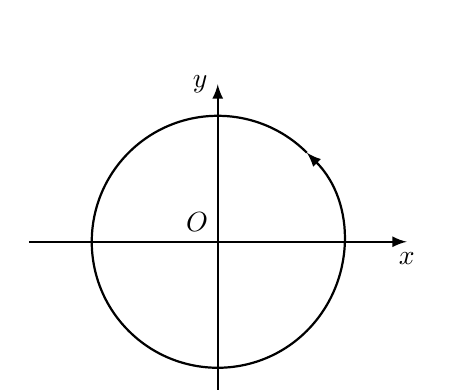
\begin{tikzpicture}[scale=.8]
		\draw[thick, -latex](-3, 0)--(3, 0)node[below]{$x$};
		\draw[thick, -latex](0, -2.5)--(0, 2.5)node[left]{$y$};
		\node[above left]at(0, 0){$O$};
		%\draw[thick, latex-latex](-2, -1.5)--(2, 1.5);
		\draw[thick, -latex](1.414, 1.414)arc(45-360:45:2);
	\end{tikzpicture}
	\tikzchap 圆偏振
\end{center}
向$-z$方向看去,($+$)对应电场终点逆时针(counterclockwise)旋转,我们称为左旋(left circular)或正螺旋性(positive helicity),因为其角动量是$+z$的;相应的($-$)对应顺时针旋转,称为右旋或负螺旋性。

%线偏振和椭圆偏振还有另一种表示,
%定义一对复矢量
依此定义圆偏振基:
\begin{equation}
    \uvec\epsilon_\pm:=\frac1{\sqrt2}(\uvec\epsilon_1\pm\i\uvec\epsilon_2),
\end{equation}
则$\uvec n,\uvec\epsilon_\pm$也是两两正交的单位矢量(复矢量内积)。在这一对坐标下
\begin{gather*}
    \bm E=(E_+\uvec\epsilon_++E_-\uvec\epsilon_-)\e{\i(\bm k\cdot\bm x-\omega t)},\\
    E_+=a_+\e{\i\vd_+},\quad E_-=a_-\e{\i\vd_-}.
\end{gather*}
若$E_\pm$相位相同但幅值不同,则$\bm E$是椭圆偏振的,长短轴在$\uvec\epsilon_{1,2}$上,且长短轴之比由$E_\pm$之比给出:
\[
    \frac{1+r}{1-r},\quad r:=\frac{E_-}{E_+};
\]
若$E_\pm$连相位也不同,则$E_-/E_+=r\e{\i\alpha}$,$\bm E$仍是椭圆偏振的,但长轴要旋转$\alpha/2$的角度。

若$E_\pm$幅值相同,则$\bm E$是线偏振的;若$E_\pm$有一个为0,则$\bm E$是圆偏振的。
\paragraph{Stokes参数}
我们如何从观察光束的细节来确定偏振的状态?对于一束光来说,
\begin{equation}
    \uvec\epsilon_1\cdot\bm E,\quad\uvec\epsilon_2\cdot\bm E;\quad\uvec\epsilon_+\cj\cdot\bm E,\quad\uvec\epsilon_-\cj\cdot\bm E,
\end{equation}
分别是沿$\uvec\epsilon_{1,2}$方向线偏振的、左旋和右旋圆偏振的振幅。这些振幅的平方给出了各类偏振强度的一种测量。%为体现幅值和相位因素,记
%我们给出相对于线偏振基和相对于圆偏振基的斯托克斯参数的定义,把这些参数用投影振幅(7.25)来表示,并且还直接用诸分量的幅值和相对位相来表示.为了达到后一目的,我们把(7.19)和(7.24)中的各标量系数定义为一

在线偏振基$\uvec\epsilon_{1,2}$下,Stokes参数表示为
\begin{equation}
    \begin{cases}
        s_0=|\uvec\epsilon_1\cdot\bm E|^2+|\uvec\epsilon_2\cdot\bm E|^2=a_1^2+a_2^2\\
        s_1=|\uvec\epsilon_1\cdot\bm E|^2-|\uvec\epsilon_2\cdot\bm E|^2=a_1^2-a_2^2\\
        s_2=2\Re\bigfkh{(\uvec\epsilon_1\cdot\bm E)\cj(\uvec\epsilon_2\cdot\bm E)}=2a_1a_2\cos(\vd_2-\vd_1)\\
        s_3=2\Im\bigfkh{(\uvec\epsilon_1\cdot\bm E)\cj(\uvec\epsilon_2\cdot\bm E)}=2a_1a_2\sin(\vd_2-\vd_1)
    \end{cases}
\end{equation}
在圆偏振基$\uvec\epsilon_\pm$下,Stokes参数表示为
\begin{equation}
    \begin{cases}
        s_0=|\uvec\epsilon_+\cj\cdot\bm E|^2+|\uvec\epsilon_-\cj\cdot\bm E|^2=a_+^2+a_-^2\\
        s_1=2\Re\bigfkh{(\uvec\epsilon_+\cj\cdot\bm E)\cj(\uvec\epsilon_-\cj\cdot\bm E)}=2a_+a_-\cos(\vd_--\vd_+)\\
        s_2=2\Im\bigfkh{(\uvec\epsilon_+\cj\cdot\bm E)\cj(\uvec\epsilon_-\cj\cdot\bm E)}=2a_+a_-\sin(\vd_--\vd_+)\\
        s_3=|\uvec\epsilon_+\cj\cdot\bm E|^2-|\uvec\epsilon_-\cj\cdot\bm E|^2=a_+^2-a_-^2
    \end{cases}
\end{equation}
Stokes参数仅依赖于$a_1,a_2,\vd_1-\vd_2$三个参数,因此并不独立,有关系:
\[
    s_0^2=s_1^2+s_2^2+s_3^2.
\]
特别的,下面给出了一些Stokes参数的例子:
\begin{compactitem}
	\item 线偏振:
    \begin{compactitem}
        \item 水平(horizontal)和垂直(vertical):$[1\enspace\pm 1\enspace0\enspace0];$
        \item $\pm 45\degree$:$[1\enspace0\enspace\pm 1\enspace0];$
    \end{compactitem}
	\item 圆偏振:右旋和左旋
	\[
        [1\enspace0\enspace0\enspace\pm 1];
    \]
	\item 无偏振(unpolarized)光或自然光(natural light):$\bm E$由无数个无规则取向的偏振光叠加,各方向振幅相同,因此$s_1,s_2,s_3$均为零
    \[
        [1\enspace0\enspace0\enspace0].
    \]
    现实中即使是%目前应用的
    单色性(monochromatic)很好的辐射波束也是由有限波列(finite wave trains)叠加成的,因而根据Fourier定理,它包含一个频率范围,即不完全是单色的。%一种看法认为$a_i,\vd_i$随时间变化缓慢,
    这时可观测的Stokes参数就是在一个较长时间尺度上的平均,比如:
    \[
        s_2=2\ave{a_1a_2\cos(\vd_2-\vd_1)},
    \]
    求平均的结果是:准单色波束的Stokes参数满足不等式:
    \[
        s_0^2\geqslant s_1^2+s_2^2+s_3^2,
    \]
\end{compactitem}
定义偏振度
\[
    P:=\frac{I_\text{elp}}{I\tot}=\frac{\sqrt{s_1^2+s_2^2+s_3^2}}{s_0},
\]
显然$0\leqslant P\leqslant 1$,
\begin{compactitem}
	\item $P=1$时对应完全偏振光;
	\item $P=0$对应无偏振光;
	\item $0<P<1$对应部分偏振光(partially polarized),这时尽管$\bm E$含有各种振动方向的光矢量,但在某一方向更显著,不难表达为无偏振光和完全偏振光的叠加:
    \[
        \begin{bmatrix}
            s_0\\s_1\\s_2\\s_3
        \end{bmatrix}_\text{pp}=(1-P)
        \begin{bmatrix}
            s_0\\0\\0\\0
        \end{bmatrix}_\text{unp}+P
        \begin{bmatrix}
            s_0\\s_1'\\s_2'\\s_3'
        \end{bmatrix}_\text{elp}.
    \]
\end{compactitem}
\paragraph{Stokes参数的测量}
Stokes参数在场强上是二次的,只能通过强度测量来确定,并结合线偏振器(linear polarizer)和四分之一波片(quarter waveplate)。线偏振器利用物质的材料特性让透射光只有沿着特定方向偏振的分量透过,而四分之一波片利用了晶体的双折射(birefringence)现象\footnote{一束光线进入某种晶体会产生两束折射光。改变入射角,其中一束光在晶体内的光速各向同性,称为o光(ordinary);而另一束光的光速各向异性,称为e光(extraordinary)。}使得o光和e光产生相位差,控制波片厚度便可以使线偏振光变成圆偏振光。

可以证明,如果线偏振器与偏振方向夹角为$\theta$,波片的相位差为$\phi$,则出射光的光强为
\[
    I(\theta,\phi)=\frac12(s_0+s_1\cos2\theta+s_2\sin2\theta\cos\phi-s_3\sin2\theta\sin\phi),
\]
\begin{compactitem}
	\item 线偏振器$\theta=0,I(0,0)=(s_0+s_1)/2;$
    \item 线偏振器$\theta=90\degree,I(90,0)=(s_0-s_1)/2;$
    \item 线偏振器$\theta=45\degree,I(45,0)=(s_0+s_2)/2;$
    \item 1/4波片+线偏振器$\theta=45\degree,I(45,45)=(s_0-s_3)/2.$
\end{compactitem}
\subsection{反射与折射}
光入射(incident)到不同媒质的分界面上会发生反射(reflect)和折射(refract)。
\begin{center}
	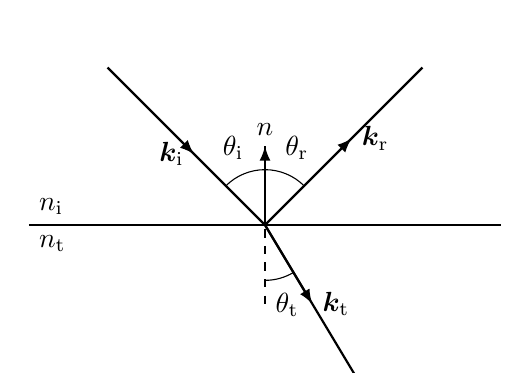
\begin{tikzpicture}
		\coordinate(O)at(0, 0);
		\coordinate(n)at(0, 1);
		\coordinate(u)at(0, -1);
		\coordinate(i)at(-2, 2);
		\coordinate(r)at(2, 2);
		\coordinate(t)at(1.2, -2);
		\draw[thick](-3, 0)node[above right]{$n_\i$}node[below right]{$n_\t$}--(3, 0);
		\draw[dashed](n)--(u);
		\draw[thick, -latex](O)--(n)node[above]{$\uvec n$};
		\draw[thick, -latex](O)--(1.1, 1.1)node[right]{$\bm k_\r$};
		\draw[thick](1, 1)--(r);
		\draw[thick, -latex](i)--(-.9, .9)node[left]{$\bm k_\i$};
		\draw[thick, -latex](-1, 1)--(O)--(.6, -1)node[right]{$\bm k_\t$};
		\draw[thick](O)--(t);
		\pic["$\theta_\i$", draw, angle eccentricity=1.5, angle radius=20]{angle=n--O--i};
		\pic["$\theta_\r$", draw, angle eccentricity=1.5, angle radius=20]{angle=r--O--n};
		\pic["$\theta_\t$", draw, angle eccentricity=1.5, angle radius=20]{angle=u--O--t};
	\end{tikzpicture}
	\tikzchap 入射波、反射波和折射波
\end{center}
入射波、反射波和折射波(或透射波transmit)的波数分别为$k_\i,k_\r,k_\t$。由前文的结论,边界上电场的切向分量是连续的:
\[
    (\bm E_\i+\bm E_\r-\bm E_\t)\times\uvec n=\bm 0.
\]
上式对任意$t$均成立,因此
\begin{equation}
    \label{eqn:omegai=omegar=omegat}
    \omega_\i=\omega_\r=\omega_\t=\omega,
\end{equation}
式(\ref{eqn:omegai=omegar=omegat})说明,不论光怎样被散射,都具有相同的频率;

又上式对分界面上的任意一点$\bm x$均成立,故
\[
    \bm k_\i\cdot\bm x=\bm k_\r\cdot\bm x+\delta_\r=\bm k_\t\cdot\bm x+\delta_\t.
\]
从前两项可以得到
\[
    (\bm k_\i-\bm k_\r)\cdot\bm x=\delta_\r,
\]
由内积的投影性质,$\bm x$的终点会扫过一个垂直于$(\bm k_\i-\bm k_\r)$的平面,而$\bm x$的终点正好在分界面上,因此$(\bm k_\i-\bm k_\r)$垂直于分界面:
\[
    (\bm k_\i-\bm k_\r)\times\uvec n=\bm 0,
\]
上述关系当然对第三项也适用,因此:$\bm k_\i,\bm k_\r,\bm k_\t$均与$\uvec n$共面,且三者的切向分量相等:
\begin{equation}
    k_\i\sin\theta_\i=k_\r\sin\theta_\r=k_\t\sin\theta_\t,
\end{equation}
而入射波与反射波在同一介质中,当然有$k_\i=k_\r$,可得反射定律
\begin{equation}
    \theta_\i=\theta_\r;
\end{equation}
入射波与折射波在不同介质中,但二者频率相同,同乘$c/\omega$得到Snell定律
\begin{equation}
    \label{eqn:Snell}
    n_\i\sin\theta_\i=n_\t\sin\theta_\t.
\end{equation}
\paragraph{Fresnel公式}
由边界上:$\bm D$和$\bm B$法向分量连续,$\bm E$和$\bm H$切向分量连续。在应用这些边界条件时,可以考虑线偏振的两种独立情况:
\begin{compactenum}
	\item $\bm E_\i$与入射面垂直(即$\bm E_\i$垂直纸面向外)%\footnote{在讨论Fresnel公式之前,我们必须指定$\bm E_\i$的方向。}
	\begin{align*}
        E_\i+E_\r&=E_\t,\\
        H_\i\cos\theta_\i-H_\r\cos\theta_\r&=H_\t\cos\theta_\t,
    \end{align*}
    通常我们处理的是$\mu_\i=\mu_\r\approx\mu_\t\approx\mu_0$的电介质,因此
    \begin{align}
        \label{eqn:Fresnel rperp}
        r_\perp:=\frac{E_\r}{E_\i}=\frac{n_\i\cos\theta_\i-n_\t\cos\theta_\t}{n_\i\cos\theta_\i+n_\t\cos\theta_\t},\\
        \label{eqn:Fresnel tperp}
        t_\perp:=\frac{E_\t}{E_\i}=\frac{2n_\i\cos\theta_\i}{n_\i\cos\theta_\i+n_\t\cos\theta_\t};
    \end{align}
    $r,t$称为振幅反射系数和透射系数;
	\item $\bm E_\i$与入射面平行(或者说$\bm H_\i$垂直纸面向外)
	\begin{align*}
        E_\i\cos\theta_\i-E_\r\cos\theta_\r&=E_\t\cos\theta_\t,\\
        H_\i+H_\r&=H_\t,
    \end{align*}
    得到 
    \begin{align}
        \label{eqn:Fresnel rpara}
        r_\parallel&=\frac{n_\t\cos\theta_\i-n_\i\cos\theta_\t}{n_\t\cos\theta_\i+n_\i\cos\theta_\t},\\
        \label{eqn:Fresnel tpara}
        t_\parallel&=\frac{2n_\i\cos\theta_\i}{n_\t\cos\theta_\i+n_\i\cos\theta_\t}.
    \end{align}
\end{compactenum}
利用Snell定律(\ref{eqn:Snell}),$r,t$便完全由$n_\i,n_\t,\theta_\i$决定。
\paragraph{Brewster角}
对于平行于入射面的偏振光,存在一个入射角$i_\text B$使得$r_\parallel=0$,%依(\ref{eqn:Fresnel rpara})
\[
    n_\t\cos\theta_\i-n_\i\cos\theta_\t=0,\quad n_\i\sin\theta_\i=n_\t\sin\theta_\t.
    %n_\t^2\cos i_\text B=n_\i\sqrt{n_\t^2-n_\i^2\sin^2 i_\text B},
\]
我们称为Brewster角
\begin{equation}
    \label{eqn:Brewster}
    \theta_\text B=\arctan\Bigkh{\frac{n_\t}{n_\i}}.
\end{equation}
玻璃相对于空气的$n_\t/n_\i=1.5$,得到$\theta_\text B=56.3\degree$。
\paragraph{全反射}
前面的讨论在绝大程度上只限于外反射($n_\i<n_\t$)的情形,即光疏介质入射光密介质。相反的情况是内反射($n_\i>n_\t$),这时$\theta_\i<\theta_\t$。
考虑$\theta_\t\geqslant90\degree$,即光疏介质没有折射光,我们称之为全反射(total internal reflection),由Snell定律,全反射的临界角
\begin{equation}
    \label{eqn:total reflect}
    \theta\c=\arcsin\Bigkh{\frac{n_\t}{n_\i}}.
\end{equation}
发生全反射时,折射角的正弦
\[
    \sin\theta_\t=\frac{n_\i}{n_\t}\sin\theta_\i=\frac{\sin\theta_\i}{\sin\theta\c}>1,
\]
则$\cos\theta_\t$是纯虚的,
\[
    \e{\i\bm k'\cdot\bm x}=\e{\i k_\t(x\sin\theta_\t+z\cos\theta_\t)},
\]
此时折射波在光疏介质内仅平行于表面传播,并在垂直方向上呈指数衰减,Poynting矢量的法向分量在时间平均上为0:
\[
    \bm S\cdot\uvec n=\frac12\Re[(\bm E\times\bm H\cj)\cdot\uvec n]=\frac1{2\omega\mu'}\Re[(\bm k'\cdot\uvec n)|\bm E'_0|^2]=0.
\]
\paragraph{Goos-Haenchen效应}
发生全反射时,光疏介质中的
倏逝波(evanescent wave)在垂直方向上以$\e{-z/\delta}$衰减,其中
\[
    \delta\iv:=k'\sqrt{\sin^2\theta_\i-\sin^2\theta\c}.
\]
如果有限横向范围内的光束经历全反射,则反射光将相对几何反射光束出现横向偏移。对于线偏振光,偏移的距离称为Goos-Haenchen偏移
\[
    D\simeq 2\delta\sin\theta_\i.
\]
\paragraph{Fresnel菱体}
发生全反射时,
反射光相对入射光的相位差为$n_\t\cos\theta_\t$,是一个纯虚数,与入射角$\theta_\i$和折射率$n_\i,n_\t$有关,这种相位差可以用来将一种偏振态的光转化为另一种偏振态,Fresnel菱体(rhombus)便是以此为原理,将垂直于表面入射的线偏振光转换为出射的圆偏振光。

经过复杂的计算,如果要实现此效果,需要满足
\[
    \cos^2\theta_\i+\frac{n_\t^2}{n_\i^2}\sin^2\theta_\i-1=\pm\,2(n_\t^2-n_\i^2)\cos\theta_\i^2\sqrt{\frac{n_\t^2}{n_\i^2}\sin^2\theta_\i-1},
\]
玻璃的折射率$n=1.5$,因此内反射角位$50.2\degree$或$53.3\degree$即可满足条件。
\iffalse
\paragraph{垂直入射}
如果光是垂直界面入射的,$\theta_\i=\theta_\t=0$,则 
\begin{align*}
    r&=\frac{n_\i-n_\t}{n_\i+n_\t},\\
    t&=\frac{2n_\i}{n_\i+n_\t}.
\end{align*}
\fi
\subsection{色散}
所有介质都表现出一定的色散性,只有在有限的频率范围内,或在真空中,光的传播速度才能被视为常量。

色散的应用:能量啁啾(chirped pulse amplification)。
\paragraph{色散的简单模型}
我们忽略外加电场和局部电场之间的区别。因此,该模型只适用于密度相对较低的物质。
忽略磁场力,
由谐波力束缚和由电场作用的电荷电子的运动方程为:
\[
    -m_\elc\omega_0^2\bm x-m_\elc\gamma\dot{\bm x}-e\bm E=m_\elc\ddot{\bm x}.
\]
$-m_\elc\omega_0^2\bm x$是回复力(restoring force),$-m_\elc\gamma\dot{\bm x}$是唯象的阻尼力(damping force)。
如果振荡的振幅足够小,便可以计算电子平均位置的电场。场随频率$\omega$的简谐$\e{-\i\omega t}$变化。
则由一个电子贡献的偶极矩为:
\[
    \bm p=-e\bm x=\frac{e^2}{m_\elc(\omega_0^2-\omega^2-\i\omega\gamma)}\bm E.
\]
从微观到宏观,单位体积内有$N$个分子,每个分子由$Z$个电子;我们将分子中的电子分类,第$j$组有$f_j$个特性相同的电子,其结合频率为$\omega_j$,阻尼常数为$\gamma_j$。
代入$\bm P=\varepsilon_0\chi_\elc\bm E$和$\varepsilon_\r=1+\chi_\elc$得到
\begin{equation}
    \varepsilon_\r(\omega)=1+\frac{Ne^2}{\varepsilon_0m_\elc}\sum_j\frac{f_j}{\omega_j^2-\omega^2-\i\omega\gamma_j},
\end{equation}
在量子力学中,$f_j,\omega_j,\gamma_j$都有合适的定义,因此上面的方程准确地描述了原子对介电常数的贡献。我们称$f_j$为振子强度(oscillator strength),$\omega_j$为共振频率(resonant frequency)。
\paragraph{异色色散和共振吸收}
通常$\gamma_j\ll\omega_j$,上式可约化为
\[
    \varepsilon_\r(\omega)\simeq 1+\frac{Ne^2}{\varepsilon_0m_\elc}\sum_j\frac{f_j}{\omega_j^2-\omega^2},
\]
对于$\omega<\min(\omega_j)$的低频率下,和的贡献是正的,$\varepsilon_\r>1$;随着频率的增加,它将穿过越来越多的$\omega_j$,求和将从正到负,最后$\varepsilon_\r<1$。

当$\omega$在共振频率$\omega_j$附近时,
\[
    \varepsilon_\r(\omega)\simeq 1+\i\frac{Ne^2}{\varepsilon_0m_\elc}\sum_j\frac{f_j}{\omega\gamma_j},
\]
$\varepsilon_\r$的虚部是可观的,由于$\varepsilon_\r$的正虚部表示电磁波向介质中产生的能量耗散,因此$\Im[\varepsilon_\r(\omega)]$较大的区域称为共振吸收(resonant absorption)区域。

回忆第 \ref{sssec:Poynting in dissipative media} 节中线性色散介质中的Poynting定律(\ref{eqn:Poynting with loss}),考虑平面波的衰减(attenuation),波数是一个复数
\[
    k=\beta+\i\frac\alpha 2.
\]
其中$\alpha$是衰减常数或吸收系数,波的强度随$\e{-\alpha z}$衰减,且$\alpha\ll\beta$。由
\[
    k\simeq\frac\omega c\sqrt{\varepsilon_\r},\thus
    \begin{cases}
        \alpha\simeq\frac{\Im(\varepsilon_\r)}{\Re(\varepsilon_\r)}\beta,\\
        \beta\simeq\frac\omega c\sqrt{\Re(\varepsilon_\r)}.
    \end{cases}
\]
\paragraph{低频表现,电导}
在低频极限$\omega\to0$下,如果每个分子中电子的某些$f_0$是自由的,即$\omega_0=0$,则$\varepsilon_\r$在$\omega=0$处是奇异的。

如果自由电子的贡献被分别显示出来,
\[
    \varepsilon(\omega)=\varepsilon_\text b(\omega)+\i\frac{Ne^2f_0}{m_\elc\omega(\gamma_0-\i\omega)},
\]
其中$\varepsilon_\text b$体现其他偶极子的贡献。

我们引入电导率(conductivity) $\sigma$的概念,体现电流密度与电场强度的关系:
\[
    \bm J=\sigma\bm E,
\]
而$\bm D=\varepsilon_\text b\bm E$,故在简谐Maxwell方程下
\[
    \curl\bm H=-\i\omega\Bigkh{\varepsilon_\text b+\i\frac\sigma\omega}\bm E,
\]
故电导率也是一个复数:
\begin{equation}
    \sigma=\frac{f_0Ne^2}{m_\elc(\gamma-\i\omega)},
\end{equation} 
\begin{example}{铜的电导率}{conductivity of copper}
    铜的参数为
    \begin{align*}
        N&=\SI{8e28}{/m^3},\\
        \sigma&=\SI{5.9e7}{/\ohm.m}.
    \end{align*}
    由此得到$\gamma_0/f_0\simeq\SI{4e13}{s^{-1}}$,而$f_0\sim 1$,因此当$\omega\leqslant\SI{e11}{s^{-1}}$时,铜的导电率是实数,并且与频率无关。
\end{example}
\paragraph{高频极限,等离子体频率}
在$\omega\gg\max(\omega_j)$的高频下,
\[
    \varepsilon_\r(\omega)\simeq 1-\frac{\omega_\text p^2}{\omega^2},
\]
$\omega_\text p$是介质的等离子体频率(plasma frequency)
\begin{equation}
    \omega_\text p^2=\frac{NZe^2}{\varepsilon_0m_\elc},\quad Z=\sum_jf_j.
\end{equation}
仅取决于总电子密度$NZ$。
\begin{example}{地球电离层的短波全反射}{ionisphere}
    电离层中,电子均是自由的且阻尼可忽略不计。对于$\omega<\omega_\text p$的情形,$\varepsilon_\r\simeq 1-\omega_\text p^2/\omega^2$的关系仍成立,此时
    \[
        ck=\omega\sqrt{\varepsilon_\r}=\sqrt{\omega^2-\omega_\text p^2}.
    \]
    是纯虚的。因此低频电磁波会被电离层反射。

    地球电离层的电子密度$NZ=\SIrange{e18}{e22}{/m^3}$,故等离子体频率$\omega_\text p\simeq\SIrange{6e10}{6e12}{s^{-1}}$,$\omega=0$的衰减常数$\alpha^{-1}=\SIrange{0.2}{2e-3}{cm}$。
\end{example}
\begin{example}{金属的紫外透射现象}{ultraviolet transparency}
    对于$\omega\ll\omega_\text p$,光被完全反射;当频率$\omega$增加到$\varepsilon_\r(\omega)>0$的区间,金属便突然可以透射光,其反射率变化得很剧烈(drastically),这称为紫外透射(ultraviolet transparency)现象。
\end{example}
\paragraph{水的折射率和吸收系数随频率的变化}
在可见光范围内,水的折射率$n\sim 1.34$,吸收系数$\alpha$骤降至一个很低的值。
\subsectionstar{在电离层和磁层中的传播模型}
电磁波对等离子体中的传播会受到外部磁场的显著影响。

略
\clearpage
\subsection{群速度}
如果介质是色散的,则波的每个频率分量的相速度都不相同,能流的速度可能与相位的速度有很大的不同,甚至缺乏精确的意义。
\paragraph{一维标量波}
一维中的标量波的通解为
\[
    u(x,t)=a\e{\i(kx-\omega t)}+b\e{\i(-kx-\omega t)},
\]
由色散性质,$\omega=\omega(k)$是波数的函数。将标量波表示成Fourier变换的形式
\[
    u(x,t)=\frac1{\sqrt{2\pi}}\int\iti A(k)\e{\i(kx-\omega t)}\d k,
\]
$A(k)$描述了不同波的线性叠加的性质,
\[
    A(k)=\frac1{\sqrt{2\pi}}\int\iti u(x,0)\e{-\i kx}\d x,
\]
对于一个单色行波,$u(x,0)\sim\e{\i k_0x}$,则$A(k)=\sqrt{2\pi}\vd(k-k_0)$,从而$u(x,t)=\e{\i(k_0x-\omega_0t)}$。
\paragraph{有限波列、群速度}
对于一个有限波列(wave train),$x,k$平均值的均方根偏差$\D x,\D k$满足Fourier带宽(bandwidth)定律
\begin{equation}
    \D x\D k\geqslant\frac12,
\end{equation}
如果一个脉冲的波数谱不太广,或者一个介质中的频率对波数的依赖性较弱,则$\omega(k)$可以被展开
\[
    \omega(k)=\omega_0+\edg{\dv\omega k}_0(k-k_0)+\cdots
\]
得到 
\[
    u(x,t)\simeq u\Bigkh{x-t\edg{\dv\omega k}_0,0}\exp\biggfkh{\i\Bigkh{k_0\edg{\dv\omega k}_0-\omega_0}t},
\]
除了一个整体的相位因子,脉冲以一种没有失真的(undistorted)速度传播,称为群速度(group velocity)
\begin{equation}
    v_\text g:=\edg{\dv\omega k}_0,
\end{equation}
对于光波,以折射率$n(k)$表示更方便:
\[
    \omega(k)=\frac{ck}{n(k)},
\]
相速度
\[
    v_\varphi=\frac{\omega(k)}k=\frac c{n(k)},
\]
群速度
\[
    v_\text g=c\biggkh{\frac1n-\frac k{n^2}\dv nk}=\frac cn-\frac\omega n\dv n\omega v_\text g,
\]
得到 
\begin{equation}
    \label{eqn:gruop v}
    v_\text g=\frac c{\displaystyle n(\omega)+\omega\dv n\omega},
\end{equation}
\paragraph{群速度可以大于光速吗?}
随着频率$\omega$的增大,经过一系列共振频率,折射率$n(\omega)$将在1附近出现上升和下降的变化,我们称上升段为正常色散,下降段为反常色散(anomalous dispersion),由群速度$v_\text g$和$\d n/\d\omega$的关系(\ref{eqn:gruop v}),在反常色散中群速度是可以超越光速的,但这并不违反相对论,个人的解释是这种群速度是波包是速度,并不传递信息。\footnote{唐老师课上讲的词忘了。}
\paragraph{进一步讨论群速度的有效性}
考虑频率对波数依赖的特定模型,并在不近似的情况下计算脉冲在该模型介质中的传播。$t=0$时标量波的初始值和初始变化率为$u(x,0),\dot u(x,0)$,则 
\[
    A(k)=\frac1{\sqrt{2\pi}}\int\iti\biggfkh{u(x,0)+\i\frac{\dot u(x,0)}{\omega(k)}}\e{-\i kx}\d x,
\]
\begin{example}{Gauss波包}{Gaussian modulated oscillation}
    考虑初始为Gauss调制振荡:
    \[
        u(x,0)=\e{-x^2/2L^2}\cos(k_0x),
    \]
    若假设$\dot u(x,0)=0$,则
    \[
        u(x,t)=\e{-x^2/2L^2}\cosh(kx-\omega t);
    \]
    \tcblower
    假设 
    \[
        \omega(k)=v\Bigkh{1+\frac{a^2k^2}2},
    \]
    则群速度
    \[
        v_\text g=\dv\omega k(k_0)=va^2k_0.
    \]
\end{example}
\subsection{\textit{\textbf{D}}和\textit{\textbf{E}}之间的因果关系}
静态电磁场
\[
    D_\alpha=\varepsilon_0E_\alpha+P_\alpha-\sum_\beta\pv{\mathcal Q'_{\alpha\beta}}{x_\beta}+\cdots
\]
若考虑时间,
会发生什么变化?
\paragraph{时间非局域性}
在色散介质中,$\varepsilon(\omega)$对频率$\omega$的依赖会导致$\bm D(\bm x,t)$和$\bm E(\bm x,t)$的临时性非局域联系。对于$\omega$的单色成分,
\[
    \hat{\bm D}(\bm x,\omega)=\varepsilon(\omega)\hat{\bm E}(\bm x,\omega),
\]
Fourier变换得到
\[
    \bm D(\bm x,t)=\frac1{2\pi}\int\iti\varepsilon(\omega)\biggfkh{\int\iti\bm E(\bm x,t')\e{\i\omega t'}\d t'}\e{-\i\omega t}\d\omega,
\]
假设积分的次序可以交换,可以得到
\begin{equation}
    \label{eqn:D-E with omega}
    \bm D(\bm x,t)=\varepsilon_0\biggfkh{\bm E(\bm x,t)+\int\iti\bm E(\bm x,t-\tau)G(\tau)\d\tau},
\end{equation}
其中 
\[
    G(\tau)=\frac1{2\pi}\int\iti\bigfkh{\varepsilon_\r(\omega)-1}\e{-\i\omega\tau}\d\omega,
\]
因此$t$时刻的$\bm D(\bm x,t)$依赖除$t$以外的电场$\bm E(\bm x,t-\tau)$。若$\varepsilon$是不依赖于$\omega$的,则 
\[
    G(\tau)=(\varepsilon_\r-1)\vd(\tau),\quad\bm D(\bm x,t)=\varepsilon\bm E(\bm x,t),
\]
$\bm D(\bm x,t)$和$\bm E(\bm x,t)$有瞬时的联系;但如果$\varepsilon(\omega)$随$\omega$变化,则$G(\tau)$在$\tau\neq 0$的一些地方也不会消失。
\paragraph{$G(\tau)$的简单模型}
假设所有的电子都以一个频率$\omega_0$振荡,则 
\[
    \varepsilon_\r(\omega)=1+\frac{\omega_\text p^2}{\omega_0^2-\omega^2-\i\gamma\omega},
\]
即 
\[
    G(\tau)=\frac{\omega_\text p^2}{2\pi}\int\iti\frac{\e{-\i\omega\tau}\d\omega}{\omega_0^2-\omega^2-\i\gamma\omega}.
\]
被积函数在$\omega$的下半平面上有两个奇点
\[
    \omega_\pm=-\i\frac\gamma 2\pm\nu_0,\quad\nu_0^2=\omega_0^2-\frac{\gamma^2}4.
\]
利用复变函数中对留数的处理,得到
\[
    G(\tau)=\omega_\text p^2\frac{\sin\nu_0\tau}{\nu_0}\e{-\gamma\tau/2},\quad\tau>0.
\]
若没有上述假设,$G(\tau)$也仅仅是上式的线性组合。因此,$\bm D(\bm x,t)$和$\bm E(\bm x,t)$之间连接上的非局域性被限制在$\gamma\iv$的时间内。而$\gamma\iv$的典型值为$\SI{e-7}{e-9}s$。

上面的方程在时间(而非空间)上是非局部的,。
\paragraph{$\varepsilon(\omega)$的因果性和分析性域}
$\tau<0$时$G(\tau)=0$。说明只有在$t$时间之前的电场$\bm E$进入以确定电位移$\bm D$,这符合我们在物理现象中的因果关系的基本思想。

假设:空间局域、线性、因果关系,均匀各向同性介质。
\paragraph{Kramers-Kronig关系}
由Cauchy定理
\begin{align*}
    \varepsilon_\r(\omega)-1&=\frac1{2\pi\i}\oint_C\frac{\varepsilon_\r(\omega')-1}{\omega'-\omega}\d\omega'\\
    &=\frac1{2\pi\i}\lim_{\delta\to0^+}\int\iti\frac{\varepsilon_\r(\omega')-1}{\omega'-\omega-\i\delta}\d\omega'
\end{align*}
由Sokhotski-Plemelj定理
\[
    \lim_{\delta\to0^+}\frac1{x\pm\i\delta}=\mathrm{P.V.}\Bigkh{\frac1x}\mp\i\pi\vd(x),
\]
故
\[
    \varepsilon_\r(\omega)=1+\frac1{\pi\i}\,\mathrm{P.V.}\int\iti\frac{\varepsilon_\r(\omega')-1}{\omega'-\omega}\d\omega'
\]
由$\Re[\varepsilon_\r(\omega)]$为偶,$\Im[\varepsilon_\r(\omega)]$为奇,得到Kramers-Kronig关系
\begin{equation}
    \begin{aligned}
        \Re[\varepsilon_\r(\omega)]&=1+\frac1\pi\,\mathrm{P.V.}\int\iti\frac{\Im[\varepsilon_\r(\omega)]}{\omega'-\omega}\d\omega'\\
        \Im[\varepsilon_\r(\omega)]&=-\frac1\pi\,\mathrm{P.V.}\int\iti\frac{\Re[\varepsilon_\r(\omega)]-1}{\omega'-\omega}\d\omega'\\
    \end{aligned}
\end{equation}
或
\begin{equation}
    \begin{aligned}
        \Re[\varepsilon_\r(\omega)]&=1+\frac2\pi\,\mathrm{P.V.}\int\zti\frac{\omega'\Im[\varepsilon_\r(\omega)]}{\omega'^2-\omega^2}\d\omega'\\
        \Im[\varepsilon_\r(\omega)]&=-\frac{2\omega}\pi\,\mathrm{P.V.}\int\zti\frac{\Re[\varepsilon_\r(\omega)]-1}{\omega'^2-\omega^2}\d\omega'\\
    \end{aligned}
\end{equation}
Kramers-Kronig关系具有非常普遍的有效性,这仅仅是根据极化和电场之间的因果关系(\ref{eqn:D-E with omega})的假设而得出的。

对于$\omega=\omega_0$处的一条非常窄的吸收线或吸收带,由
\begin{align*}
    \Im[\varepsilon_\r(\omega)]&\simeq\frac{\pi K}{2\omega_0}\vd(\omega'-\omega_0)+\cdots\\
    \Re[\varepsilon_\r(\omega)]&\simeq\bar\varepsilon+\frac K{\omega_0^2-\omega^2},
\end{align*}
\clearpage
\section{波导}
\label{sec:waveguide}
%有金属边界存在时的电磁场,是一个具有实用价值的相当重要的题材。
在波长的数量级为数米或更短一些的高频情况下,产生和发送电磁波的唯一实用的方法,是利用线度可以与有关波长相比的金属结构。我们在本章里先考虑在一个导体附近的场,并讨论场对表面的穿透以及伴随着的电阻损失,然后用相当普遍的观点讨论中空金属管导引的电磁波和谐振腔等问题,而且在讨论的过程中引进特殊例子来说明这些问题。用两种不同观点讨论波导中的衰减和谐振腔的$Q$值。%其次把地球-电离层系统当作新奇的谐振腔来处理,接着简短地讨论电介质波导。我们还阐述波导中任意场的简正模展开,并应用到定域源产生的场。本章最后把简正模展开进一步应用到用变分法处理波导中障碍物问题。

\subsection{导体介质的场}
理想导体(perfect conductor)和超导体(superconductor)的异同?
最大的不同是不存在理想导体,但存在超导体。

理想导体表面电荷密度为$\varsigma$、表面电流密度为$\bm K$,理想导体外的电位移$\bm D$和磁场强度$\bm H$满足
\[
    \uvec n\cdot\bm D=\varsigma,\quad\uvec n\times\bm H=\bm K.
\]
在理想导体表面,仅存在法向的$\bm E$和切向的$\bm H$,并且这两个场在理想导体内骤降为0。

对于非理想的良导体,导体内的场随趋肤深度
\begin{equation}
    \delta:=\sqrt{\frac2{\mu\c\omega\sigma}}.
\end{equation}
指数衰减,且
其电导率$\sigma$是一个有限量,而Ohm定律$\bm J=\sigma\bm E$说明表面没有电流$\bm K$。边界条件应改为
\[
    \uvec n\times(\bm H-\bm H\c)=\bm 0,
\]
由于场在垂直于表面的方向上的空间变化比平行方向快得多,因此和法向导数相比,切向导数可以忽略。若$\xi$表示导体向内的法向坐标,则
\[
    \nabla\simeq-\uvec n\pp\xi.
\]
忽略导体内的位移电流,谐振场的Maxwell方程变为
\begin{align*}
    \bm E\c&\simeq\frac1\sigma\curl\bm H\c\simeq-\frac1\sigma\uvec n\times\pv{\bm H\c}\xi,\\
    \bm H\c&=-\i\frac1{\mu\c\omega}\curl\bm E\c\simeq\i\frac1{\mu\c\omega}\uvec n\times\pv{\bm E\c}\xi.
\end{align*}
变形得到
\begin{align*}
    \Bigkh{\pp[2]\xi+\i\frac2{\delta^2}}(\uvec n\times\bm H\c)&\simeq\bm 0,\\
    \uvec n\cdot\bm H\c&\simeq 0.
\end{align*}
第二个方程表面:导体内$\bm H$平行于表面,这与边界条件相符。解得
\begin{equation}
    \bm H\c=\bm H_\parallel\e{-\xi/\delta}\e{\i\xi/\delta}.
\end{equation}
$\bm H_\parallel$是导体外表面的切向磁场,则导体内电场
\begin{equation}
    \bm E\c\simeq\sqrt{\frac{\mu\c\omega}{2\sigma}}(1-\i)(\uvec n\times\bm H_\parallel)\e{-\xi/\delta}\e{\i\xi/\delta}.
\end{equation}
故导体内的$\bm H\c$和$\bm E\c$与表面平行,大小随指数迅速衰减,二者有相位差,且磁场比电场强得多。在表面外侧,除了法向的$\bm E$和切向的$\bm H$外,还有$\bm E$的一个微小的切向分量存在。这意味着有功率流入导体,每单位面积的吸收对时间平均的功率是
\begin{equation}
    \dv{P_\text{loss}}a=-\frac12\Re[\uvec n\cdot(\bm E\times\bm H\cj)]=\frac{\mu\c\omega\delta}4|\bm H_\parallel|^2.
\end{equation}
可把这个结果简单地解释为导体内的Ohm损失,由Ohm定律,导体表面附件有电流密度$\bm J=\sigma\bm E\c$,而
\[
    \dv{P_\text{loss}}V=\frac12\bm J\cdot\bm E\cj=\frac\sigma 2|\bm J|^2.
\]
定义有效面电流密度
\[
    \bm K\eff:=\int\zti\bm J\d\xi=\uvec n\times\bm H_\parallel.
\]
则
\[
    \dv{P_\text{loss}}a=\frac1{2\sigma\delta}|\bm K\eff|^2.
\]
\subsection{柱形空腔和波导}
电磁波在中空的金属柱体内的传播或激发,是一种极为重要的实用情形。如果柱体具有端面,就叫做空腔(cavity),否则就叫做波导(waveguide)。在我们讨论这问题时,都假定柱体的边界面是理想导体,在实际应用中发生的能量损失,可用上一节的方法来估计。

假定柱形曲面$S$的截面形状和大小沿柱体轴不变,且柱体内是介电常数$\varepsilon$、磁导率$\mu$的均匀非耗散介质。当柱体内的场具有谐振关系$\e{-\i\omega t}$时,Maxwell方程组可化为以下形式:
\begin{alignat*}{2}
    \div\bm E&=0,&\qquad\curl\bm E&=\i\omega\bm B,\\
    \div\bm B&=0,&\curl\bm B&=-\i\mu\varepsilon\omega\bm E.
\end{alignat*}
即
\[
    (\lapla+\mu\varepsilon\omega^2)\bm E=\bm 0,
\]
由边界限制,单独考虑$z$方向上的空间变化:
\[
    \bm E(x,y,z,t)=\bm E(x,y)\e{\i(\pm kz-\omega t)},
\]
由适当的线性组合可以给出沿$z$方向的行波或驻波,目前,波数$k$是一个未知参数,它可能是实数也可能是复数。假定了场对$z$有上述依赖关系后,波动方程就简化为二维形式:
\[
    (\lapla_\t+\mu\varepsilon\omega^2-k^2)\bm E=0,
\]
其中$\lapla_\t$表示Laplace算符的横向部分:
\[
    \lapla_\t:=\lapla-\pp[2]z,
\]
再将场分解为平行和垂直于$z$轴两个分量$\bm E=\bm E_z+\bm E_\t$:
\[
    \bm E_z=E_z\uvec z,\quad\bm E_\t=(\uvec z\times\bm E)\times\uvec z.
\]
Maxwell方程组变为
\begin{alignat*}{2}
    \nabla_\t\cdot\bm E_\t&=-\pv{E_z}z,&\qquad\qquad\nabla_\t\cdot\bm B_\t&=-\pv{B_z}z,\\
    \pv{\bm E_\t}z+\i\omega\uvec z\times\bm B_\t&=\nabla_\t E_z,&\uvec z\cdot(\nabla_\t\times\bm E_\t)&=\i\omega\bm B_z,\\
    \pv{\bm B_\t}z-\i\mu\varepsilon\omega\uvec z\times\bm E_\t&=\nabla_\t B_z,&\uvec z\cdot(\nabla_\t\times\bm B_\t)&=\i\mu\varepsilon\omega\bm E_z.
\end{alignat*}
因此$\bm E_\t,\bm B_\t$可以被$E_z,B_z$确定
\begin{align}
    \bm E_\t&=\i\frac1{\mu\varepsilon\omega^2-k^2}(k\nabla_\t E_z-\omega\uvec z\times\nabla_\t B_z),\\
    \bm B_\t&=\i\frac1{\mu\varepsilon\omega^2-k^2}(k\nabla_\t B_z+\mu\varepsilon\omega\uvec z\times\nabla_\t E_z),
\end{align}
\paragraph{TEM模}
在讨论中空柱体内可以存在的各种场之前,我们先说一说简并型或特殊型解,即所谓横电磁(TEM)波。这种解只有垂直于传播方向的横场分量,$E_z=B_z=0,\enspace\bm E_\t=\bm E_\text{TEM}$且
\begin{equation}
    \nabla_\t\times\bm E_\text{TEM}=\bm 0,\quad\nabla_\t\cdot\bm E_\text{TEM}=0.
\end{equation}
因此$\bm E_\text{TEM}$是二维静电问题的一个解。由此可得轴向波数为
\begin{equation}
    \label{eqn:TEM k0}
    k_0=\omega\sqrt{\mu\varepsilon},
\end{equation}
磁场 
\[
    \bm B_\text{TEM}=\pm\sqrt{\mu\varepsilon}\uvec z\times\bm E_\text{TEM},
\]
电导率为无穷大的单个中空柱形导体内不可能存在TEM模。为了运载TEM模,必须有两个及以上的圆柱面(等势面)。TEM模的一个重要性质是不存在截止频率,即对任意$\omega$,$k$均是实数。
\paragraph{TM波和TE波}
在中空柱体内(以及高频时的传输线上)出现两类场的构型。考虑纵向分量$E_z$和$B_z$满足的波动方程以及边界条件,就可以看出这两类场的构型的存在。对于理想导电柱体,边界条件是
\[
    \uvec n\times\bm E=\bm0,\quad\uvec n\cdot\bm B=0,
\]
显然$E_z$的边界条件为
\begin{equation}
    E_z|_S=0,
\end{equation}
相应的$B_z$的边界条件是
\begin{equation}
    \edg{\pv{B_z}n}_S=0,
\end{equation}
对于给定频率$\omega$来说,波数$k$只可以出现某些值(波导情况);或对于给定波数$k$来说,只允许某些$\omega$值(谐振腔)。由于$E_z$和$B_z$边界条件不同,所以一般来说本征值是不同的,因此场自然分为两种类型:
\begin{compactitem}
	\item TE波:处处$B_z=0$,边界条件$E_z|_S=0;$
	\item TM波:处处$E_z=0$,边界条件$\p B_z/\p n|_S=0.$
\end{compactitem}
\subsection{波导}
当波在一个均匀截面的中空波导中传播时,可得TM波和TE波的横磁场和横电场的关系如下:
\[
    \bm H_\t=\pm\frac1Z\uvec z\times\bm E_\t,
\]
$Z$为波阻抗,
\[
    Z:=\begin{cases}
        \frac k{\varepsilon\omega}=\frac k{k_0}\sqrt{\frac\mu\varepsilon},&\text{TM}\\
        \frac {\mu\omega}k=\frac {k_0}k\sqrt{\frac\mu\varepsilon},&\text{TE}
    \end{cases}
\]
这里$k_0$由(\ref{eqn:TEM k0})给出。
横向场可由纵向场决定
\begin{alignat*}{2}
    \text{TM}&:\quad&\bm E_\t&=\pm\i\frac k{\gamma^2}\nabla_\t\psi,\quad E_z=\psi\e{\pm\i kz};\\
    \text{TE}&:\quad&\bm H_\t&=\pm\i\frac k{\gamma^2}\nabla_\t\psi,\quad H_z=\psi\e{\pm\i kz}.
\end{alignat*}
式中$\gamma^2=\mu\varepsilon\omega^2-k^2$,标量函数$\psi$满足二维波动方程
\[
    (\lapla_\t+\gamma^2)\psi=0,
\]
边界条件:
\[
    \text{TM}:\enspace\psi|_S=0;\qquad\text{TE}:\enspace\edg{\pv\psi n}_S=0.
\]
可以确定一系列本征值$\gamma_\lambda$和本征函数$\psi_\lambda$,这些不同的解称为波导的波模。对于给定的频率$\omega$,每个$\lambda$对应的波数
\[
    k_\lambda^2=\mu\varepsilon\frac{\omega^2}{c^2}-\gamma_\lambda^2.
\]
定义截止频率(cutoff frequency):
\begin{equation}
    \label{eqn:cutoff omega}
    \omega_\lambda:=\frac{\gamma_\lambda}{\sqrt{\mu\varepsilon}},
\end{equation}
则上式可以写成
\[
    k_\lambda=\sqrt{\mu\varepsilon}\sqrt{\omega^2-\omega_\lambda^2}.
\]
截止频率的意义为:
\begin{compactitem}
    \item 当$\omega>\omega_\lambda$时,$k_\lambda$是实数,$\lambda$模的波可以在波导中传播;
    \item 当$\omega<\omega_\lambda$时,$k_\lambda$是虚数,$\lambda$模的波不能传播。
\end{compactitem}
因此给定频率上,只有有限个波模可以传播。选择波导的尺寸,使得在使用频率上只能出现最低波模的波,这往往是最方便的。

波导中的波长总是大于自由空间中的波长,因此相速度就大于无限空间中的值
\[
    v_\varphi=\frac\omega{k_\lambda}=\frac c{\sqrt{\mu\varepsilon}}\frac1{\sqrt{1-(\omega_\lambda/\omega)^2}}>\frac c{\sqrt{\mu\varepsilon}}.
\]
\subsubsection{矩形波导中的波模}
我们考虑矩形波导中的TE波:$E_z=0,\,H_z=\psi$
\begin{example}{矩形波导中的波模}{modes in a rectangular waveguide}
    在内尺寸为$a,b$的矩形波导中,
    \[
        \Bigkh{\pp[2]x+\pp[2]y+\gamma^2}\psi=0,
    \]
    边界上$\p\psi/\p n=0$可得
    \[
        \psi_{mn}=H_0\cos\Bigkh{\frac{m\pi x}a}\cos\Bigkh{\frac{n\pi y}b},\quad\gamma_{mn}^2=\pi^2\Bigkh{\frac{m^2}{a^2}+\frac{n^2}{b^2}}.
    \]
    不失一般性取$a>b$,则TE模的最低截止频率为$m=1,\,n=0$
    \[
        \omega_{10}=\frac\pi{\sqrt{\mu\varepsilon}a}.
    \]
    %对应波长$\lambda_{10}=2a\sqrt{\mu\varepsilon}/c$,
    在自由空间(即波导中没有介质)中正好$\lambda_{10}=2a$。将TE$_{10}$的场写出:
    \begin{align*}
        H_z&=H_0\cos\Bigkh{\frac{\pi x}a}\e{\i(kz-\omega t)},\\
        H_x&=-\i\frac{ka}\pi H_0\sin\Bigkh{\frac{\pi x}a}\e{\i(kz-\omega t)},\\
        E_y&=\i\frac{\omega a\mu}\pi H_0\sin\Bigkh{\frac{\pi x}a}\e{\i(kz-\omega t)}.
    \end{align*}
    $\i$说明传播方向上$H_x,E_y$与$H_z$有$90\degree$的相位差。
    \tcblower
    TM波:
    \[
        E_z=E_0\sin\Bigkh{\frac{m\pi x}a}\sin\Bigkh{\frac{n\pi y}a},
    \]
    最低波模为$m=n=1$。
\end{example}
\subsubsection{波导中的能流和衰减}
我们扩大前面对任意截面形状的柱形波导所作的一般讨论,使它包括沿波导的能流以及波的衰减,后者是当电导率有限时由波导管壁中能量损耗所引起的。我们只限于讨论波导中只存在一种波模的情况;不过将简短提一下简并波模。能流用复Poynting矢量描写;
\begin{equation}
    \bm S=\frac12\bm E\times\bm H\cj=\frac{\omega k}{2\gamma^4}
    \begin{cases}
        \varepsilon\Bigkh{\uvec z|\nabla_\t\psi|^2+\i\frac{\gamma^2}k\psi\nabla_\t\psi\cj},&\text{TM}\\[1ex]
        \mu\Bigkh{\uvec z|\nabla_\t\psi|^2-\i\frac{\gamma^2}k\psi\cj\nabla_\t\psi},&\text{TE}
    \end{cases}
\end{equation}
因为$\psi$一般是实数,\footnote{有可能这样激发一个波导,使得某给定波模或一些波模的线性组合具有复数$\psi$。这时候横向能流对时间的平均值将不为零,但因为它是一个环流,所以实际上只代表贮藏的能量,在实用上不大重要。}
因此$\bm S$的第二项代表无功能流,并且对能流的时间平均没有贡献。总功率流
\[
    P=\int_A\bm S\cdot\uvec z\d a=\frac{\omega k}{2\gamma^4}
    \begin{Bmatrix}
        \varepsilon\\\mu
    \end{Bmatrix}
    \biggkh{\oint_{\p A}\cancel{\psi\cj\pv\psi n}\d\ell-\int_A\psi\cj\nabla_\t^2\psi\d a}.
\]
由特征方程$(\nabla_\t^2+\gamma_\lambda^2)\psi=0$,
\[
    P=\frac1{2\sqrt{\mu\varepsilon}}\biggkh{\frac\omega{\omega_\lambda}}^2\biggkh{1-\frac{\omega_\lambda^2}{\omega^2}}^{1/2}
    \begin{Bmatrix}
        \varepsilon\\\mu
    \end{Bmatrix}
    \int_A\psi\cj\psi\d a.
\]
时间平均能量密度
\[
    u=\frac14\Bigkh{\varepsilon\bm E\cdot\bm E\cj+\frac1\mu\bm B\cdot\bm B\cj},
\]
单位长度的场能量
\[
    U=\frac12\biggkh{\frac\omega{\omega_\lambda}}^2
    \begin{Bmatrix}
        \varepsilon\\\mu
    \end{Bmatrix}
    \int_A\psi\cj\psi\d a,
\]
能流的速度正是群速度
\[
    \frac PU=\frac k\omega\frac1{\mu\varepsilon}=\frac1{\sqrt{\mu\varepsilon}}\sqrt{1-\frac{\omega_\lambda^2}{\omega^2}}=v_\text g.
\]
结合前面说的相速度
\begin{equation}
    v_\text gv_\varphi=\frac1{\mu\varepsilon},
\end{equation}
在无限介质中,$v_\text g$总是小于$v_\varphi$,并且在截止频率时降为零。
\paragraph{良导体的波导}
对于理想导体,$k_\lambda$是实数或纯虚数;而对于电导率有限的良导体来说,$k_\lambda$是一个实数与一个小复数的和。

后面的略。
\paragraph{最小衰减频率}
略。
\subsection{边界条件的扰动}
略
\subsection{谐振腔}
一个谐振腔(resonant cavity)可以是任何形状的,具有一个封闭的导体表面。但通常我们将端面放置在一个长度的圆柱形波导上,以产生一个空腔。端面是垂直于圆柱体轴线的平面。
\subsection{腔内的功率损失}
品质因子(quality factor)
\begin{equation}
    Q:=\omega_0\frac{\text{stored energy}}{\text{power loss}}.
\end{equation}
\clearpage
\section{多极辐射}
\label{sec:multipole radiation}
在第七章和第八章里,讨论了电磁波的性质,以及电磁波在有界的和无界的区域内的传播情况。但是,很少谈到如何产生这些电磁波的问题。本章就转入这个问题,并讨论定域振荡电荷和电流密度系统辐射的电磁波,我们的论述是直截了当的,而不去精心推敲数学形式。%当然,这样做只限于比较简单的辐射系统,我们把求系统辐射的渐近法(用任意$l$的矢量多极场)推迟到第十六章里论述。本章只讨论电偶极子、磁偶极子和电器极子,以及导体上电流的一些简单位形。也论述波导中一个源的简单多极子展开和孔的有效多极矩。

%本章后半部,用较大篇幅讨论散射和衍射。首先解释长波长情形下的散射,包括瑞利对蓝天的解释和有关的论题,然后讨论标量衍射理论和矢量衍射理论,并举了一些例子。最后讨论短波长情形下的散射和重要的光学定理。
\subsection{局域振荡源}
对于随时间变化的电荷和电流系统,我们都可以将随时间变化的量作Fourier分析,并分别处理各个Fourier分量。因此,不失一般性,我们只考虑随时间作正弦变化的局域电荷和电流系统所产生的势、场和辐射,设
\begin{align*}
    \rho(\bm x,t)&=\rho(\bm x)\e{-\i\omega t},\\
    \bm J(\bm x,t)&=\bm J(\bm x)\e{-\i\omega t},
\end{align*}
矢量势
\begin{align}
    \notag
    \bm A(\bm x,t)&=\frac{\mu_0}{4\pi}\int\frac{\bm J(\bm x',t')}{|\bm x-\bm x'|}\vd\Bigkh{t'-t+\frac{|\bm x-\bm x'|}c}\d t'\nd v'\\
    \label{eqn:A-Jeiwt}
    &=\frac{\mu_0}{4\pi}\int\frac{\bm J(\bm x')}{|\bm x-\bm x'|}\e{\i k|\bm x-\bm x'|}\d v'.
\end{align}
磁场和电场为
\[
    \bm H=\frac1{\mu_0}\curl\bm A,\quad\bm E=\i\frac Zk\curl\bm H.
\]
给定电流分布$\bm J(\bm x')$以后,至少在原则上可以通过计算(\ref{eqn:A-Jeiwt})的积分来定出场的分布。%9.4节将讨论一两个直接计算源积分的实例.
但是,现在我们先确立在电流源被局限于小区域内(与波长相比,确实很小)的极限情形下,场所具有的某些简单而普遍的性质。如果源的线度为$d$,波长为$\lambda=2\pi c/\omega$,并且$d<\lambda$,则有三个令人感兴趣的空间区域:近区、中间区、远区。

近区:$d\ll r\ll\lambda$,(\ref{eqn:A-Jeiwt})中的指数可以用1代替,并用球谐函数(\ref{eqn:1/|x-x'|=YY})展开,
\[
    \lim_{kr\to0}\bm A(\bm x)=\frac{\mu_0}{4\pi}\sum_{\ell=0}^\infty\sum_{m=-\ell}^\ell\frac{4\pi}{2\ell+1}\frac{Y_{\ell m}(\theta,\phi)}{r^{\ell+1}}\int\bm J(\bm x')r'^\ell Y\cj_{\ell m}(\theta',\phi')\d v'.
\]
上式表明,近场是准静态的,除了按$\e{-\i\omega t}$方式作简谐振荡外,其它性质都是静态的。

远区,$d\ll\lambda\ll r$,
\[
    \bm A(\bm x,t)=\frac{\mu_0}{4\pi}\frac{\e{\i kr}}r\int\bm J(\bm x')\e{-\i\bm k\cdot\bm x'}\d v'.
\]
可以对$\e{-\i\bm k\cdot\bm x'}$展开,略。

中间区,$d\ll r\sim\lambda$,近似失效,引入
球Bessel函数和Hankel函数
\begin{align}
    j_\ell(x)&:=\sqrt{\frac\pi{2x}}J_{\ell+1/2}(x),\\
    y_\ell(x)&:=\sqrt{\frac\pi{2x}}Y_{\ell+1/2}(x),\\
    h^\pm_\ell(x)&:=j_\ell(x)\pm\i y_\ell(x).
\end{align}
则
\[
    \bm A(\bm x)=\i\mu_0k\sum_{\ell,m}h_\ell^+(kr)Y_{\ell m}(\theta,\phi)\int\bm J(\bm x')j_\ell(kr')Y\cj_{\ell m}(\theta',\phi')\d v',
\]
推导和后面的略。

标量势与矢量势形式相同,我们考虑电单极的情况
\[
    \Phi(\bm x,t)=\frac1{4\pi\varepsilon_0r}q\Bigkh{t-\frac rc},
\]
式中$q(t)$是源的总电荷。因为电荷是守恒的,且根据定义,局域源是一个没有电荷流入或流出的源,所以总电荷$q$与时间无关。于是,一个定域源的势(和场)的电单极部分必然是静态的。%具有谐和时间依赖关系e-'(w≠0)的场没有单极子项。

%现在讨论w≠0时最低阶多极场。因为这些场可以由矢势通过(9.4)和(9.5)算出,所以我们在下面的论述中不再明显提及标势。
\subsection{电偶极辐射}
下面我们求电偶极子
\[
    \bm p:=\int\bm x'\rho(\bm x')\d v',
\]
激发的电场和磁场。
通过远区近似,
\[
    \bm A=-\i\frac{\mu_0\omega}{4\pi}\bm p\frac{\e{\i kr}}r.
\]
场
\begin{align*}
    \bm H&=\frac{ck^2}{4\pi}(\uvec n\times\bm p)\frac{\e{\i kr}}r\Bigkh{1+\i\frac1{kr}},\\
    \bm E&=\frac1{4\pi\varepsilon_0}\biggfkh{k^2(\uvec n\times\bm p)\times\uvec n\frac{\e{\i kr}}r+\bigkh{3\uvec n(\uvec n\cdot\bm p)-\bm p}\Bigkh{\frac1{r^3}-\i\frac{k}{r^2}}\e{\i kr}}.
\end{align*}
$r\to 0$时,
\begin{align*}
    \bm H&=\i\frac{\omega}{4\pi}\frac{\uvec n\times\bm p}{r^2},\\
    \bm E&=\frac1{4\pi\varepsilon_0}\frac{3\uvec n(\uvec n\cdot\bm p)-\bm p}{r^3};
\end{align*}
$r\to\infty$时,
\begin{align*}
    \bm H&=\frac{ck^2}{4\pi}(\uvec n\times\bm p)\frac{\e{\i kr}}r,\\
    \bm E&=Z_0\bm H\times\uvec n.
\end{align*}
由振荡偶极子辐射的时间平均功率
\[
    \dv P\Omega=\frac12\Re\bigfkh{r^2(\bm E\times\bm H\cj)\cdot\uvec n}=\frac{c^2Z_0}{32\pi^2}k^4p^2\sin^2\theta,
\]
故
\begin{equation}
    P=\frac{c^2Z_0^2k^4}{12\pi}p^2.
\end{equation}
为什么天空是蓝色的,特别是在垂直于太阳光线的天弧处?因为$\theta=90\degree$时太阳光线所激发的偶极辐射功率为0。
\begin{example}{天线}{center-fed, linear antenna}
    对于一个中间馈送(center-fed)的线性天线(antenna),其电流
    \[
        I_0\Bigkh{1-\frac{2|z|}d}\e{-\i\omega t},
    \]
    则其电偶极矩为
    \[
        p=\i\frac{I_0d}{2\omega},
    \]
    辐射功率
    \[
        P=\frac{Z_0I_0^2}{48\pi}(kd)^2.
    \]
    由于天线向外辐射功率,因此它需要消耗能量,尽管天线是一个理想导体,但仍有辐射阻抗$R_\text{rad}$,由$Z_0\simeq\SI{377}{\ohm}$
    \[
        R_\text{rad}=\frac{Z_0}{24\pi}(kd)^2\simeq 5(kd)^2.
    \]
\end{example}
\subsection{磁偶极子和电四极子}
\paragraph{磁偶极子}
磁偶极矩对矢量势的贡献
\[
    \bm A=\frac{k\mu_0}{4\pi}(\uvec n\times\bm m)\frac{\e{\i kr}}r\Bigkh{\i-\frac1{kr}},
\]
得到磁场和电场
\begin{align*}
    \bm H&=\frac1{4\pi}\biggfkh{k^2(\uvec n\times\bm m)\times\uvec n\frac{\e{\i kr}}r+\bigkh{3\uvec n(\uvec n\cdot\bm m)-\bm m}\Bigkh{\frac1{r^3}-\i\frac{k}{r^2}}\e{\i kr}},\\
    \bm E&=-\frac{Z_0}{4\pi}k^2(\uvec n\times\bm m)\frac{\e{\i kr}}r\Bigkh{1+\i\frac1{ kr}}.
\end{align*}
与电偶极子形式高度相似。
\paragraph{电四极子}
电四极子对矢量势的贡献
\[
    \bm A=-\frac{\mu_0ck^2}{8\pi}\frac{\e{\i kr}}r\Bigkh{1+\i\frac1{kr}}\int\bm x'(\uvec n\cdot\bm x)\rho(\bm x')\d v'.
\]
磁场
\[
    \bm H=-\i\frac{ck^3}{24\pi}\frac{\e{\i kr}}r\uvec n\times(\mathcal Q\cdot\uvec n).
\]
辐射功率 
\[
    \dv P\Omega=\frac{c^2Z_0}{1152\pi^2}k^6\abs{\bigfkh{\uvec n\times(\mathcal Q\cdot\uvec n)}\times\uvec n}^2
\]
从而 
\[
    P=\frac{c^2Z_0k^6}{1440\pi}\sum_{\alpha,\beta}|\mathcal Q_{\alpha\beta}|^2\sim\omega^6.
\]

\clearpage
\section{相对论电动力学}
\label{sec:relativistic electromagnetic}
%三维一般波动方程
%\lapla u-\frac1{a^2}\pv[2]ut=-f(\bm x,t),
%中的$a$是波速,依惯性系而不同。
\paragraph{Michelson-Morley实验}
人们最开始假设光和声音一样,都需要某种介质来支持它的传播。最初假想光是在一种叫作以太(ether)的媒介中传播的,光在相对于以太以不同状态运动时会有不同的速度。为了验证以太是否存在以及光速是否是常数,1887年Michelson和Morley设计了如下所示的光学干涉装置:
\begin{center}
	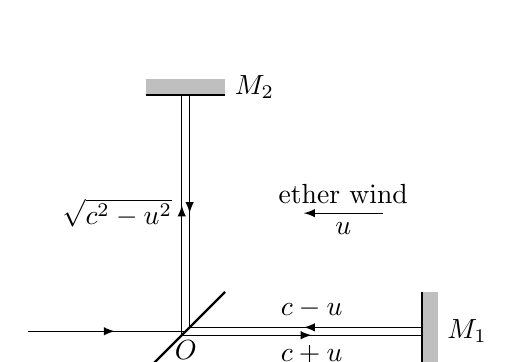
\begin{tikzpicture}
		\draw[-latex](0, 0)--(1.1, 0);
		\draw(1, 0)--(2, 0)node[below]{$O$};
		\draw[thick](2-.5, -.5)--(2.5, .5);
		\draw[-latex](2-.05, -.05)--(3.6, -.05)node[below]{$c+u$};
		\draw(3.5, -.05)--(5, -.05);
		\draw(2.05, .05)--(3.6, .05)node[above]{$c-u$};
		\draw[latex-](3.5, .05)--(5, .05);
		\fill[gray!50](5, .5)rectangle(5.2, -.5);
		\node[right]at(5.2, 0){$M_1$};
		\draw[thick](5, .5)--(5, -.5);
		\draw[-latex](2-.05, -.05)--(2-.05, 1.6);
		\draw(2-.05, 1.5)node[left]{$\sqrt{c^2-u^2}$}--(2-.05, 3);
		\draw(2.05, .05)--(2.05, 1.6);
		\draw[latex-](2.05, 1.5)--(2.05, 3);
		\fill[gray!50](1.5, 3)rectangle(2.5, 3.2);
		\node[right]at(2.5, 3.1){$M_2$};
		\draw[thick](1.5, 3)--(2.5, 3);
		\draw[latex-](3.5, 1.5)--(4.5, 1.5)node[midway, below]{$u$}node[midway, above]{ether wind};
	\end{tikzpicture}
	\tikzchap Michelson-Morley光学干涉仪的实验装置图
	%\label{pic:Michelson-Morley}
\end{center}
图中最左侧相干光源发出的光在经过中央的一个半透射半反射的膜$O$后,其中一半的光被透射后抵达镜子$M_1$然后被反射回$O$点,另一半的光被反射后抵达镜子$M_2$然后被反射回$O$点,并与从$M_1$反射回来的光发生干涉。假设整个装置在以太中以速度$u$向右运动,那么这等价于装置不动,而以太风以速度$u$向左吹来。%我们可以把“以太风”想象成是一条水流速度为$u$向左均匀流动的河流,把光想象成是一艘固有速度是$c$的船。那么
容易得出光在水平方向从$O$到$M_1$再返回$O$的路径上所花费的时间是:
\[
	T_1=\frac L{c-u}+\frac L{c+u}=\frac{2L/c}{1-u^2/c^2}.
\]
同理,容易得出光在竖直方向上从$O$到$M_2$再返回$O$的路径上所花费的时间是:
\[
	T_2=\frac{2L}{\sqrt{c^2-u^2}}=\frac{2L/c}{\sqrt{1-u^2/c^2}}.
\]
容易发现$T_1\neq T_2$。为了简化计算,假设装置在以太中的运动速度$u\ll c$,那么我们可以对小量做Taylor展开得出光沿着两条路径上传播的时间差是:
\[
	T_1-T_2\simeq\frac{2L}c\biggkh{1+\frac{u^2}{c^2}}-\frac{2L}c\biggkh{1+\frac{u^2}{2c^2}}=\frac{Lu^2}{c^3}.
\]
由于光沿着两条路径传播存在着如上所示的时间差,即存在所谓光程差,所以我们自然预期在实验观测中会发现光学干涉条纹的偏移。然而,最终的实验结果发现光学干涉条纹并未发生任何改变,%也就是说上述的时间差结果是0!
而且把光学桌旋转一定角度后发现干涉条纹依然没有发生任何改变!这也就从实验上证明了以太并不存在,光速恒为常数$c$!
\subsection{狭义相对论}
略去大部分内容,尺缩、钟慢等。仅介绍Lorentz变换:%\footnote{为了之后计算方便,也为了更好地凸显出理论的对称性,我们把$c$这个常数定义成1,也就是把光速$c$定义成一个标准单位.这样处理后时间和空间的量纲也统一起来了}
\begin{equation}
	\begin{bmatrix}
		ct'\\x'\\y'\\z'
	\end{bmatrix}=
	\begin{bmatrix}
		\gamma&\gamma\beta\\-\gamma\beta&\gamma\\ &&1\\ &&&1
	\end{bmatrix}
	\begin{bmatrix}
		ct\\x\\y\\z
	\end{bmatrix}
\end{equation}
其中$\beta:=v/c,\enspace\gamma:=1/\sqrt{1-\beta^2}$。$v$为$S'$系相对于$S$系的速度。

如果质点在$S$系中有速度$u=\d x/\d t$,则其在$S'$中的速度为
\[
    u'=\dv{x'}{t'}=\frac{\gamma(\d x-v\d t)}{\gamma(\d t-v\d t/c^2)}=\frac{u-v}{1-vu/c^2}.
\]
\paragraph{时空结构}
为讨论形式的统一,我们定义四矢量的各个分量
\[
    x^0:=ct,\enspace x^1:=x,\enspace x^2:=y,\enspace x^3:=z.
\]
则Lorentz变换可以表示为\footnote{使用Einstein求和约定,比如下式表示$\nu$取$0,1,2,3$的和。}
\[
    \bar x^\mu=\Lambda^\mu{}_\nu x^\nu.
\]
我们可推广四矢量,定义逆变量(contravariant)
\[
    a^\mu:=(a^0,a^1,a^2,a^3)\tp,
\]
和协变量(covariant)
\[
    a_\mu:=(a_0,a_1,a_2,a_3)\equiv(-a^0,a^1,a^2,a^3).
\]
四维标量积
\[
    a_\mu b^\mu:=a_0b^0+a_1b^1+a_2b^2+a_3b^3\equiv a^\mu b_\mu.
\]

假设事件$A,B$发生在$(x_A^0,x_A^1,x_A^2,x_A^3)$和$(x_B^0,x_B^1,x_B^2,x_B^3)$,定义四矢量位移
\[
    \D x^\mu:=x_A^\mu-x_B^\mu,
\]
二者的间隔(interval)
\[
    I:=(\D x)_\mu(\D x)^\mu=-c^2t^2+x^2+y^2+z^2,
\]
是不变的。
\[
    \bar I=I.
\]
若$I<0$,则是类时的(timelike);若$I>0$,则是类空的(spacelike);$I=0$,则是类光的(lightlike)。
\paragraph{相对论运动学}
由于钟慢效应(time dilation),在静止系中的时间流速是最慢的,可定义
固有时间(proper time)
\[
    \d\tau=\gamma\d t.
\]
4矢量速度
\begin{equation}
    \eta^\mu:=\dv{x^\mu}\tau,
\end{equation}
4矢量动量 
\[
    p^\mu=m\eta^\mu.
\]
其中$m$为静止质量,其时间(temporal)分量是$p^0=\gamma mc$,对应相对论能量
\[
    E=\gamma mc^2,
\]
静止时,$E=mc^2$,二者之差为动能
\[
    \Ek=E-mc^2\simeq\frac12mv^2+\frac38\frac{mv^4}{c^2}+\frac5{16}\frac{mv^6}{c^4}+\cdots,
\]
相对论动量
\[
    \bm p=m\eta=\gamma m\bm v.
\]
有
\begin{equation}
    E^2=p^2c^2+m^2c^4.
\end{equation}
\paragraph{不变和守恒}
不变(invariant)量表示在所有惯性系中均保持相同的值;守恒(conserved)量表示在某个过程前后保持相同的值。比如,质量是不变量,却不守恒;能量是守恒的,但不是不变量;电荷量既是不变量,又是守恒量;而速度既不是不变量,也不守恒。

在每个封闭系统中,总的相对论能量和动量都是守恒的。
\begin{example}{Compton散射}{Compton scattering}
    过程略,解得
    \[
        \D\lambda=\frac h{m_\elc c}(1-\cos\theta),
    \]
\end{example}
\paragraph{相对论动力学}
相对论中的力依然遵循Newton第二定律中的定义:
\[
    \bm F:=\dv{\bm p}t,
\]
而Newton第三定律不再成立,因为在相对论中,同时性是相对的。

如果质点在$S$系中保持静止,则其受到的力的变换为:
\begin{equation}
    \bm F_\perp'=\frac1\gamma\bm F_\perp,\qquad F_\parallel'=F_\parallel.
\end{equation}
\subsection{相对论电动力学}
为什么会有磁场?利用静电学和相对论,我们可以计算出载电流线和运动电荷之间的磁力,而不需要援引磁力定律。
\begin{example}{导线的磁场力}{}
    $S$系中有一导线,其中正负电荷线密度为$\pm\lambda$,均在导线中以速度$v$运动,则$\lambda=\gamma\lambda_0$,电流为$I=2\lambda v$,导线外距离$r$处有一电荷$q$沿平行于导线的方向以速度$u<v$运动。

    $S$系中导线没有净电荷,因此电荷$q$不受电场力。

    转换到粒子静止的参考系$S'$,则电荷$q$不受磁场力,仅受电场力。
    
    $S'$系中正负电荷的速度为
    \[
        v_\pm=\frac{v\mp u}{1\mp vu/c^2},
    \]
    正负电荷线密度变为$\lambda_\pm=\pm\gamma_{v_\pm}\lambda_0$,总电荷线密度和电场为
    \[
        \lambda\tot=-\frac{2vu}{c^2}\gamma_u\lambda,\quad E=\frac{\lambda\tot}{2\pi\varepsilon_0r}.
    \]
    因此$S'$系中电荷所受的电场力为
    \[
        F'=qE=-\frac{vu\gamma_u\lambda}{c^2}\frac q{\pi\varepsilon_0r}.
    \]
    变回到$S$系中,
    \[
        F=\frac1{\gamma_u}F'=-\frac{vu\lambda}{c^2}\frac q{\pi\varepsilon_0r}=-qu\frac{\mu_0I}{2\pi}.
    \]
    而$q$不受电场力,故此力只能是磁场力!
\end{example}
\paragraph{场的变换}
假设:
\begin{compactenum}
	\item 电荷是不变的;
	\item 无论场是如何产生的,转换规则都是相同的。
\end{compactenum}
得到
\begin{align}
    E_x'&=E_x,&E_y'&=\gamma(E_y-vB_z),&E_z'&=\gamma(E_z+vB_y);\\
    B_x'&=B_x,&B_y'&=\gamma\Bigkh{B_y+\frac v{c^2}E_z},&B_z'&=\gamma\Bigkh{B_z-\frac v{c^2}E_y}.
\end{align}
\begin{example}{匀速运动电荷的场}{E, B of q with v}
    在静止系$S'$中
    \[
        E'=\frac1{4\pi\varepsilon_0}\frac q{r'^2}\uvec r',
    \]
    变换到原系$S$
    \[
        E_x=E_x',\quad E_y=\gamma E_y',\quad E_z=\gamma E_z',
    \]
    得到电场 
    \begin{equation}
        \bm E=\frac1{4\pi\varepsilon_0}\frac{1-\beta^2}{(1-\beta^2\sin^2\theta)^{3/2}}\frac q{r^2}\uvec r.
    \end{equation}
    磁场 
    \begin{equation}
        \bm B=\frac{\bm v}{c^2}\times\bm E=\frac{\mu_0}{4\pi}\frac{(1-\beta^2)\sin\theta}{(1-\beta^2\sin^2\theta)^{3/2}}\frac{qv}{r^2}\uvec\phi.
    \end{equation}
\end{example}
\subsubsection{电磁场张量}
电磁场的变换是由一个反对称的二级张量连接起来的
\[
    t^{\mu\nu}=
    \begin{bmatrix}
        0&t^{01}&t^{02}&t^{03}\\
        -t^{01}&0&t^{12}&t^{13}\\
        -t^{02}&-t^{12}&0&t^{23}\\
        -t^{03}&-t^{13}&-t^{23}&0
    \end{bmatrix}.
\]
变换为 
\[
    \bar t^{\mu\nu}=\Lambda^\mu{}_\rho\Lambda^\nu{}_\sigma t^{\rho\sigma}.
\]
对应分量的变换规则为
\begin{align*}
    \bar t^{01}&=t^{01},&\bar t^{02}&=\gamma(t^{02}-\beta t^{12}),&\bar t^{03}&=\gamma(t^{03}+\beta t^{31}),\\
    \bar t^{23}&=t^{23},&\bar t^{31}&=\gamma(t^{31}+\beta t^{03}),&\bar t^{12}&=\gamma(t^{12}-\beta t^{02}).
\end{align*}
与场变换比较,可得电磁张量
\begin{equation}
    F^{\mu\nu}=
    \begin{bmatrix}
        0&E_x/c&E_y/c&E_z/c\\
        -E_x/c&0&B_z&-B_y\\
        -E_y/c&-B_z&0&B_x\\
        -E_z/c&B_y&-B_x&0
    \end{bmatrix}.
\end{equation}
或对偶(dual)张量
\begin{equation}
    G^{\mu\nu}=
    \begin{bmatrix}
        0&B_x&B_y&B_z\\
        -B_x&0&-E_z/c&E_y/c\\
        -B_y&E_z/c&0&-E_x/c\\
        -B_z&-E_y/c&E_x/c&0
    \end{bmatrix}.
\end{equation}
\paragraph{张量符号中的电动力学}
用张量的语言重新表述电动力学定律(Maxwell方程和Lorentz力定律)。统一电荷源$\rho$和电流源$\bm J$,定义4矢量电流源
\begin{equation}
    J^\mu=(c\rho,J_x,J_y,J_z)\tp,
\end{equation}
连续性方程(\ref{eqn:continuity})变为 
\[
    \p_\mu J^\mu:=\frac{\p J^0}{\p x^0}+\frac{\p J^1}{\p x^1}+\frac{\p J^2}{\p x^2}+\frac{\p J^3}{\p x^3}=\pv\rho t+\div\bm J=0,
\]
Maxwell方程组变为 
\begin{equation}
    \p_\nu F^{\mu\nu}=\mu_0J^\mu,\quad\p_\nu G^{\mu\nu}=0.
\end{equation}
$\mu=0$给出 
\[
    \div\bm E=\rho/\varepsilon_0,\quad\div\bm B=0;
\]
$\mu=1,2,3$给出$x,y,z$分量 
\[
    \curl\bm B-\mu_0\varepsilon_0\pv{\bm E}t=\mu_0\bm J,\quad\curl\bm E+\pv{\bm B}t=\bm0.
\]
Minkowski力 
\begin{equation}
    K^\mu:=q\eta_\nu F^{\mu\nu},
\end{equation}
得到Lorentz力的表达式
\[
    \bm F=q(\bm E+\bm u\times\bm B),
\]
\subsubsection{相对论势}
4矢量势
\begin{equation}
    A^\mu:=(\Phi/c,A_x,A_y,A_z)\tp,
\end{equation}
则电磁张量可以由
\begin{equation}
    F^{\mu\nu}=\frac{\p A^\nu}{\p x_\mu}-\frac{\p A^\mu}{\p x_\nu}=\p^\mu A^\nu-\p^\nu A^\mu.
\end{equation}
注意这里是协变量$x_\mu$,$x_0=-ct$有一个负号。
\begin{example}{匀速运动电荷的场·续}{E, B of q with v, II}
    续例 \ref{exm:E, B of q with v},我们用势的方法再做一遍。$S'$系中电荷静止 
    \[
        \Phi'=\frac1{4\pi\varepsilon_0}\frac q{r'},\quad\bm A'=\bm 0,
    \]
    变回$S$系
    \[
        \Phi=\gamma\Phi',\quad A_x=\gamma\frac v{c^2}\Phi',\quad A_y=A_z=0,
    \]
    其中 
    \[
        r'=\sqrt{x'^2+y'^2+z'^2}=\sqrt{\gamma^2x^2+y^2+z^2}.
    \]
    则
    \[
        \bm E=-\nabla\Phi-\pv{\bm A}t=\frac1{4\pi\varepsilon_0}\frac{\gamma q\bm r}{(\gamma^2x^2+y^2+z^2)^{3/2}}.
    \]
\end{example}
得
\[
    \p^\mu\p_\nu A^\nu-\p^\nu\p_\nu A^\mu=\mu_0J^\mu,
\]
使用Lorenz规范
\[
    \p_\mu A^\mu=\div\bm A+\frac1{c^2}\pv\Phi t=0.
\]
由此我们得到了Maxwell方程组最简单的形式:
\begin{equation}
    \p^\nu\p_\nu A^\mu=-\mu_0J^\mu.
\end{equation}
\iffalse
\begin{example}{}{}

\end{example}
\fi
\iffalse
\begin{compactenum}
	\item 
\end{compactenum}
\begin{compactitem}
	\item 
\end{compactitem}
\fi
\end{document}